\chapter{The Intrinsic Geometry of Surfaces}\label{chap:intrinsic-geometry}

% ==================== Section 4-1: Introduction ====================
\section{Introduction}\label{sec:intro-ch4}

\textbf{Why intrinsic geometry?} 在第 2 章中，我们引入了曲面的第一基本形式，并展示了如何利用它来计算曲面 $S$ 上的简单度量概念（长度、角度、面积等）。重要的是，这些计算可以"不离开曲面"地完成——一旦已知第一基本形式，我们就可以进行所有这些度量。这意味着这些概念是\textbf{内蕴}于曲面 $S$ 的。

然而，第一基本形式的几何并不止于这些简单概念。正如我们将在本章中看到的，曲面的许多重要局部性质只能通过第一基本形式来表达。研究这类性质的学科称为\textbf{曲面的内蕴几何}（intrinsic geometry of surfaces）。本章专门讨论内蕴几何。

\textbf{The main theme.} 第 3 章的性质是通过研究切平面在一点邻域中的变化得到的。现在，我们要类比曲线理论，为曲面上的每一点配置一个三面体（类似于曲线的 Frenet 标架），并研究其向量的导数。

\textbf{Organization of this chapter.} 本章组织如下。4-2 节定义等距（isometry）的概念，精确刻画两个曲面具有"相同"第一基本形式的含义。4-3 节证明著名的 Gauss 公式，将 Gaussian 曲率 $K$ 表示为第一基本形式系数的函数——这意味着 $K$ 是内蕴概念，一个非常惊人的事实。4-4 节开始系统研究内蕴几何，通过共变导数（covariant derivative）这一概念来统一处理。4-5 节讨论局部和整体的 Gauss-Bonnet 定理。4-6 节定义指数映射并引入法坐标和测地极坐标。4-7 节补充关于测地线的若干精细性质（初读可略过）。

\begin{Remark}
第 3 章的性质依赖于曲面在空间中的位置（第二基本形式），而本章的核心发现是：许多几何量实际上只依赖于第一基本形式——即曲面的内蕴结构。这一转变是微分几何发展史上的里程碑。
\end{Remark}

% ==================== Section 4-2: Isometries; Conformal Maps ====================
\section{Isometries; Conformal Maps}\label{sec:isometries}

\textbf{When do two surfaces have the same intrinsic geometry?} 圆柱面与平面是一个引人深思的例子。尽管圆柱面和平面是不同的曲面，但它们的第一个基本形式是"相等"的（在我们所考虑的坐标邻域中）。这意味着，就内蕴度量问题（长度、角度、面积）而言，平面和圆柱面在局部具有相同的行为。这一观察促使我们精确刻画：什么是两个正则曲面具有"相同"第一基本形式？

\begin{Definition}[等距]\label{def:isometry}
设 $S$ 和 $\bar{S}$ 是正则曲面。一个双射 $\varphi: S \to \bar{S}$ 是\textbf{等距映射}（isometry），如果对所有 $p \in S$ 和所有 $w_1, w_2 \in T_p(S)$，都有
\[
\langle w_1, w_2 \rangle_p = \langle d\varphi_p(w_1), d\varphi_p(w_2) \rangle_{\varphi(p)}.
\]
此时称 $S$ 和 $\bar{S}$ 是\textbf{等距的}（isometric）。
\end{Definition}

换句话说，等距映射 $\varphi$ 的微分 $d\varphi$ 保持内积。由此可知 $d\varphi$ 是等距映射，因此
\[
I_p(w) = \langle w, w \rangle_p = \langle d\varphi_p(w), d\varphi_p(w) \rangle_{\varphi(p)} = I_{\varphi(p)}(d\varphi_p(w))
\]
对所有 $w \in T_p(S)$ 成立。反之，若双射 $\varphi$ 保持第一基本形式，即
\[
I_p(w) = I_{\varphi(p)}(d\varphi_p(w))\quad \forall w \in T_p(S),
\]
则由极化恒等式可推出 $\varphi$ 是等距映射。

\begin{Definition}[局部等距]\label{def:local-isometry}
设 $V \subset S$ 是 $p \in S$ 的一个邻域。映射 $\varphi: V \to \bar{S}$ 称为在 $p$ 处的\textbf{局部等距映射}（local isometry at $p$），如果存在 $\varphi(p) \in \bar{S}$ 的邻域 $\bar{V}$，使得 $\varphi: V \to \bar{V}$ 是等距映射。如果对每个 $p \in S$ 都存在到 $\bar{S}$ 的局部等距映射，则称 $S$\textbf{局部等距于} $\bar{S}$。
\end{Definition}

显然，若 $\varphi: S \to \bar{S}$ 是双射且在每点均为局部等距，则 $\varphi$ 是（整体）等距。然而，两个曲面可能局部等距但整体不等距——圆柱面与平面就是如此：圆柱面去掉一条母线后可以展开到平面上，但整体来看，圆柱面与平面不同胚（圆柱面有洞），因此不存在整体等距。

\begin{figure}[H]
\centering
\begin{minipage}{0.45\textwidth}
\centering
\subfloat[Figure 4-1. 平面中的简单闭曲线可以收缩到一点]{\label{fig:fig4-1a}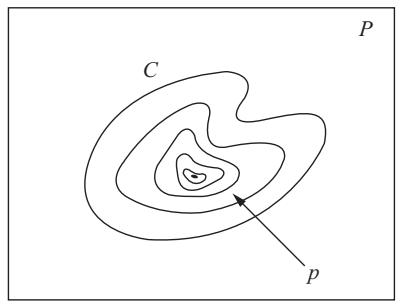
\includegraphics[width=\textwidth]{../../../PDFs/differential-geometry/transcript/Do Carmo - Differential Geometry of Curves and Surfaces/hybrid_ocr/images/0925e7f3e745e48c60981d7f3f1a5ba33e8da090624192f9883f94b6cf4a2946.jpg}}
\end{minipage}
\hfill
\begin{minipage}{0.50\textwidth}
\centering
\subfloat[Figure 4-1. 圆柱面上的平行圆不能收缩到一点]{\label{fig:fig4-1b}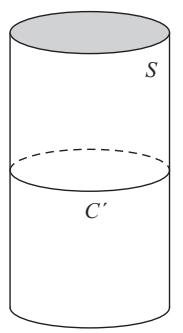
\includegraphics[width=\textwidth]{../../../PDFs/differential-geometry/transcript/Do Carmo - Differential Geometry of Curves and Surfaces/hybrid_ocr/images/eb8fd2f5d3c9703ed52411c1947234bf3148fd4f3ad861dc4a587f6e27408b95.jpg}}
\end{minipage}
\end{figure}

\begin{Proposition}[局部等距的坐标判据]\label{prop:local-isometry-criterion}
设 $\mathbf{x}: U \to S$ 和 $\bar{\mathbf{x}}: U \to \bar{S}$ 是参数化，使得在 $U$ 中 $E = \bar{E}$，$F = \bar{F}$，$G = \bar{G}$。则映射 $\varphi = \bar{\mathbf{x}} \circ \mathbf{x}^{-1}: \mathbf{x}(U) \to \bar{S}$ 是局部等距。
\end{Proposition}

\begin{Example}[圆柱面局部等距于平面]\label{ex:cylinder-plane}
教材 Figure 4-2（见 \cref{fig:fig4-2}）所示。圆柱面 $x^2 + y^2 = 1$ 在参数化 $\bar{\mathbf{x}}(u,v) = (\cos u, \sin u, v)$ 下的第一基本形式系数为 $E = 1$，$F = 0$，$G = 1$——与平面标准参数化 $\mathbf{x}(u,v) = (u, v, 0)$ 相同。因此映射 $\varphi = \mathbf{x} \circ \bar{\mathbf{x}}^{-1}$ 是局部等距。

直观上，这一等距可以通过"展开"圆柱面来实现——沿母线剪开圆柱面，即可平铺到平面上。
\end{Example}

\begin{figure}[H]
\centering
\begin{minipage}{0.60\textwidth}
\centering
\subfloat[Figure 4-2. 圆柱面与平面的局部等距]{\label{fig:fig4-2}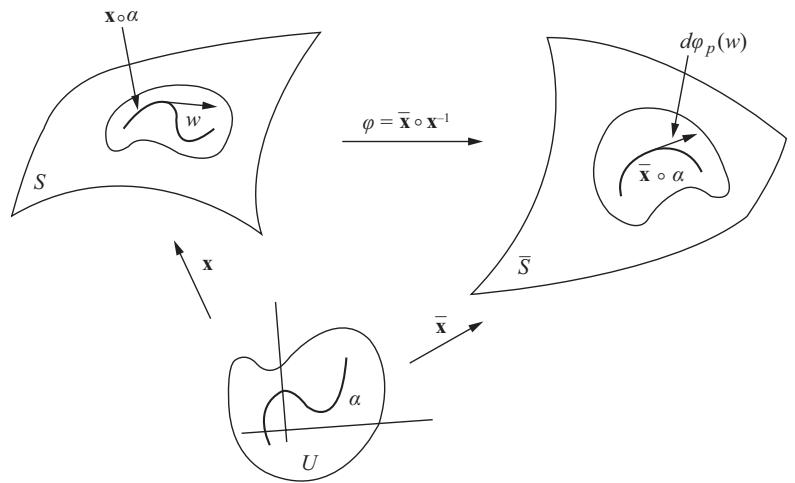
\includegraphics[width=\textwidth]{../../../PDFs/differential-geometry/transcript/Do Carmo - Differential Geometry of Curves and Surfaces/hybrid_ocr/images/6d09c1f73799a1765ba3870a22533b29be5b19a9e928f37f61a24454797080ab.jpg}}
\end{minipage}
\end{figure}

\begin{Example}[悬链面局部等距于螺旋面]\label{ex:catenoid-helicoid}
旋转面中的悬链面（catenoid）
\[
\mathbf{x}(u,v) = (a\cosh v \cos u,\; a\cosh v \sin u,\; a v),\quad 0<u<2\pi,\; -\infty<v<\infty
\]
与螺旋面（helicoid）
\[
\bar{\mathbf{x}}(u,v) = (a\sinh v \cos u,\; a\sinh v \sin u,\; a u)
\]
在变换 $\bar{u} = u$，$\bar{v} = a\sinh v$ 下具有相同的第一基本形式系数 $E = a^2\cosh^2 v$，$F = 0$，$G = a^2\cosh^2 v$。由 \cref{prop:local-isometry-criterion}，两者局部等距（教材 Figure 4-3（见 \cref{fig:fig4-3}））。

等距映射的几何意义：将螺旋面的一圈（$0<u<2\pi$）映射为去掉一条经线的悬链面（教材 Figure 4-4（见 \cref{fig:fig4-4}））。
\end{Example}

\begin{figure}[H]
\centering
\begin{minipage}{0.55\textwidth}
\centering
\subfloat[Figure 4-3. 悬链面 (catenoid)]{\label{fig:fig4-3}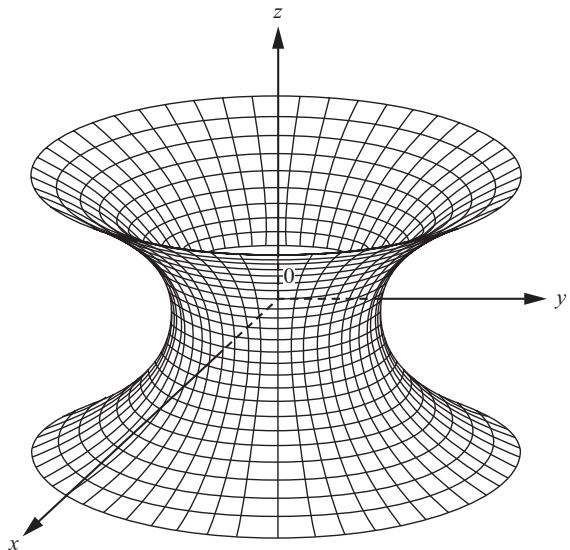
\includegraphics[width=\textwidth]{../../../PDFs/differential-geometry/transcript/Do Carmo - Differential Geometry of Curves and Surfaces/hybrid_ocr/images/df02fc7c86adc79f0710e7cfb54a79bfd51089a5aab6d7212b55a44ac5540b86.jpg}}
\end{minipage}
\end{figure}

\begin{figure}[H]
\centering
\begin{minipage}{0.30\textwidth}
\centering
\subfloat[Phase 1]{\label{fig:fig4-4a}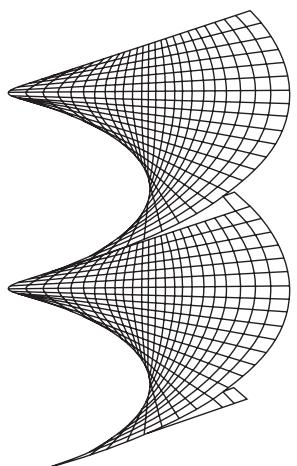
\includegraphics[width=\textwidth]{../../../PDFs/differential-geometry/transcript/Do Carmo - Differential Geometry of Curves and Surfaces/hybrid_ocr/images/0c9126aaaab80458de8a29ab28f95a6cd3c35eb26225e3537983ef88e5561b7b.jpg}}
\end{minipage}
\hfill
\begin{minipage}{0.30\textwidth}
\centering
\subfloat[Phase 2]{\label{fig:fig4-4b}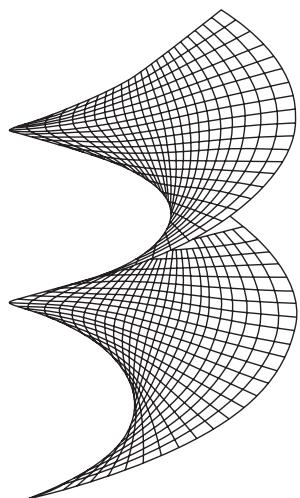
\includegraphics[width=\textwidth]{../../../PDFs/differential-geometry/transcript/Do Carmo - Differential Geometry of Curves and Surfaces/hybrid_ocr/images/93adfc01151d3f8e1199513189b1f8823b28df157a02bddc460f9ef97910a25c.jpg}}
\end{minipage}
\hfill
\begin{minipage}{0.30\textwidth}
\centering
\subfloat[Phase 3]{\label{fig:fig4-4c}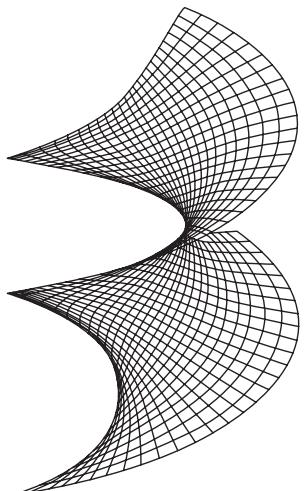
\includegraphics[width=\textwidth]{../../../PDFs/differential-geometry/transcript/Do Carmo - Differential Geometry of Curves and Surfaces/hybrid_ocr/images/31289f879dd8952044287c20b4479d2aa010f20763f0321462454ee4a9f59efe.jpg}}
\end{minipage}
\end{figure}

\begin{figure}[H]
\centering
\begin{minipage}{0.22\textwidth}
\centering
\subfloat[Phase 4]{\label{fig:fig4-4d}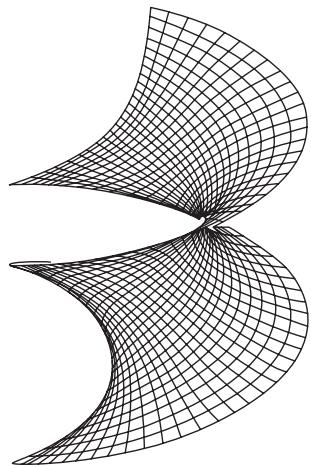
\includegraphics[width=\textwidth]{../../../PDFs/differential-geometry/transcript/Do Carmo - Differential Geometry of Curves and Surfaces/hybrid_ocr/images/34e6749e1a9c51a59379f4fabdcfe2404882e9baad2697b9d9d4fd5d0c189223.jpg}}
\end{minipage}
\hfill
\begin{minipage}{0.22\textwidth}
\centering
\subfloat[Phase 5]{\label{fig:fig4-4e}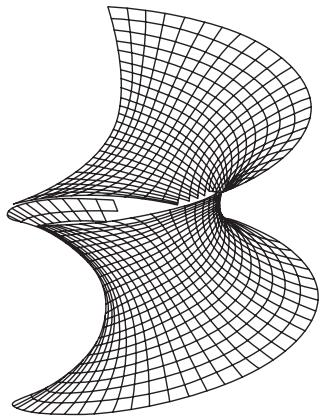
\includegraphics[width=\textwidth]{../../../PDFs/differential-geometry/transcript/Do Carmo - Differential Geometry of Curves and Surfaces/hybrid_ocr/images/b4bb3a909c3982a5964c77dfa56e6387f836635e91a493a77d20731329ba5530.jpg}}
\end{minipage}
\hfill
\begin{minipage}{0.22\textwidth}
\centering
\subfloat[Phase 6]{\label{fig:fig4-4f}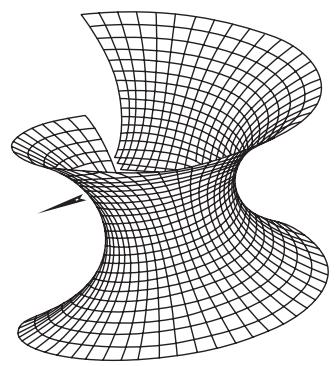
\includegraphics[width=\textwidth]{../../../PDFs/differential-geometry/transcript/Do Carmo - Differential Geometry of Curves and Surfaces/hybrid_ocr/images/9ae8400b9fe61dd40174b9aa36f0499be69823ba206362fccda45ea9f971809e.jpg}}
\end{minipage}
\hfill
\begin{minipage}{0.22\textwidth}
\centering
\subfloat[Phase 7]{\label{fig:fig4-4g}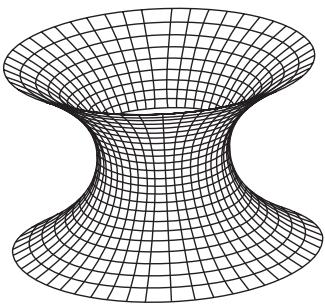
\includegraphics[width=\textwidth]{../../../PDFs/differential-geometry/transcript/Do Carmo - Differential Geometry of Curves and Surfaces/hybrid_ocr/images/00e3d20dc468132380d7bee09fd6ba5f3151e7011afbdc6b72b7a6fd004f4131.jpg}}
\end{minipage}
\end{figure}
\begin{figure}[H]
\centering
\begin{minipage}{0.60\textwidth}
\centering
\subfloat[Figure 4-4. 螺旋面到悬链面的等距形变]{\label{fig:fig4-4}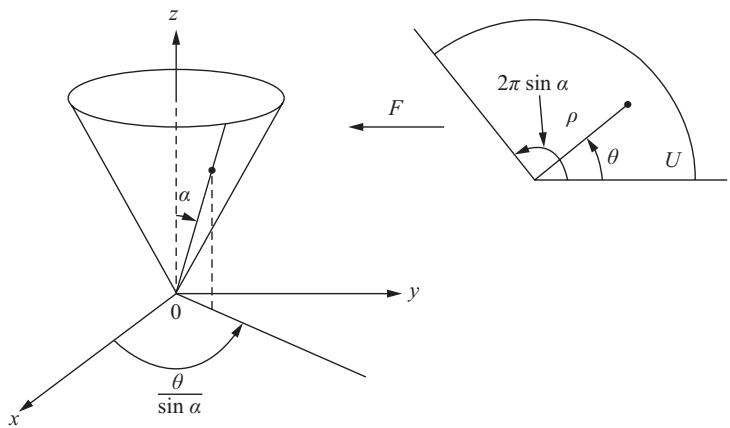
\includegraphics[width=\textwidth]{../../../PDFs/differential-geometry/transcript/Do Carmo - Differential Geometry of Curves and Surfaces/hybrid_ocr/images/6103c579eb6ce37b2e2c1443f0dea400a6ee319e2dd9952c67a5dd46f52822e0.jpg}}
\end{minipage}
\end{figure}

\begin{Example}[单叶锥面局部等距于平面]\label{ex:cone-plane}
单叶锥面（去掉顶点）$z = k\sqrt{x^2+y^2}$ 局部等距于平面。其思想是：去掉一条母线的锥面可以"滚动"到平面的一片区域（教材 Figure 4-5（见 \cref{fig:fig4-5}））。

锥面在极坐标下的参数化为
\[
f(\rho,\theta) = (\rho\sin\alpha\cos(\theta/\sin\alpha),\; \rho\sin\alpha\sin(\theta/\sin\alpha),\; \rho\cos\alpha),
\]
其中 $2\alpha$ 是锥顶角（$\cot\alpha = k$）。直接验证可得其在参数化下的第一基本形式系数为 $\bar{E}=1$，$\bar{F}=0$，$\bar{G}=\rho^2$，与平面极坐标参数化完全相同。故 $f$ 是局部等距。$\square$
\end{Example}

\begin{figure}[H]
\centering
\begin{minipage}{0.60\textwidth}
\centering
\subfloat[Figure 4-5. 锥面等距展开到平面]{\label{fig:fig4-5}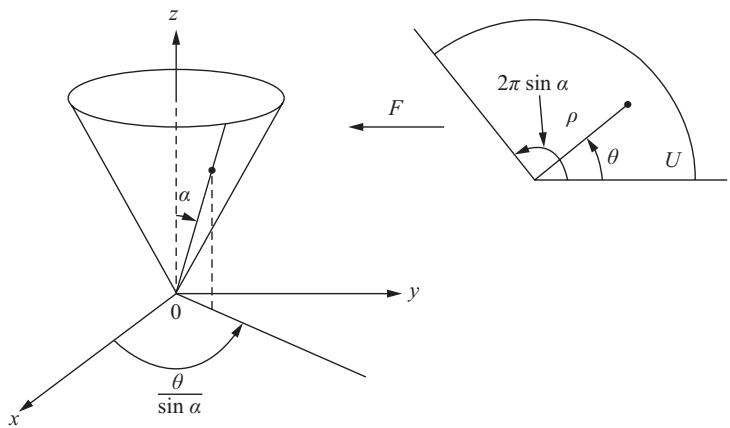
\includegraphics[width=\textwidth]{../../../PDFs/differential-geometry/transcript/Do Carmo - Differential Geometry of Curves and Surfaces/hybrid_ocr/images/6103c579eb6ce37b2e2c1443f0dea400a6ee319e2dd9952c67a5dd46f52822e0.jpg}}
\end{minipage}
\end{figure}

\textbf{Conformal maps.} 等距是度量等价的最强概念。在研究解析函数时，另一个重要概念是共形（保角）映射。

\begin{Definition}[共形映射]\label{def:conformal-map}
双射 $\varphi: S \to \bar{S}$ 称为\textbf{共形映射}（conformal map），如果对所有 $p \in S$ 和所有 $v_1, v_2 \in T_p(S)$，都有
\[
\langle d\varphi_p(v_1), d\varphi_p(v_2) \rangle = \lambda^2(p) \langle v_1, v_2 \rangle_p,
\]
其中 $\lambda^2$ 是 $S$ 上无处为零的可微函数。此时称 $S$ 和 $\bar{S}$ 是\textbf{共形的}（conformal）。
\end{Definition}

共形映射的几何意义：它保持角度（但不一定保持长度）。事实上，两曲线在 $\varphi$ 下的夹角不变。

\begin{Theorem}[任何两个正则曲面局部共形]\labelthm:local-conformal}
任意两个正则曲面局部共形。
\end{Theorem}
证明基于等温参数化（isothermal parametrization）的存在性——即可以将邻域参数化使得 $E = G = \lambda^2(u,v)$，$F = 0$。

\begin{Remark}
等距显然是共形映射的特例（$\lambda \equiv 1$）。等距 $\Rightarrow$ 保长 $\Rightarrow$ 保角；但反过来，共形映射不一定保长，因此两个曲面可能共形但不等距（如球面与平面通过球极投影共形）。
\end{Remark}

\begin{Remark}
利用第一基本形式，我们可以引入曲面上两点之间的内蕴距离。设 $d(p,q)$ 为连接 $p$ 与 $q$ 的曲线上弧长的下确界。等距映射保持内蕴距离（教材 Figure 4-6（见 \cref{fig:fig4-6}））。
\end{Remark}

\begin{figure}[H]
\centering
\begin{minipage}{0.60\textwidth}
\centering
\subfloat[Figure 4-6. 内蕴距离与欧氏距离的关系]{\label{fig:fig4-6}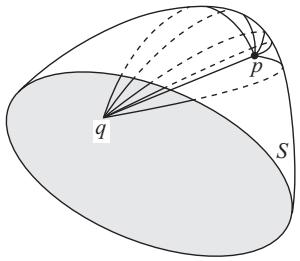
\includegraphics[width=\textwidth]{../../../PDFs/differential-geometry/transcript/Do Carmo - Differential Geometry of Curves and Surfaces/hybrid_ocr/images/a584e96933f72f8c17d816019494436bb48803bb96af1ca63462e4969371d15f.jpg}}
\end{minipage}
\end{figure}

\begin{Remark}
Mercator 投影是球面到平面的共形映射的一个经典例子（见习题 16）。它将球面的经纬线映射为平面上的直线，且保持角度——这就是为什么 Mercator 地图上直线航线（等角航线）与真实最短航路不同。
\end{Remark}

\begin{figure}[H]
\centering
\begin{minipage}{0.60\textwidth}
\centering
\subfloat[Figure 4-7. Mercator 投影保持角度]{\label{fig:fig4-7}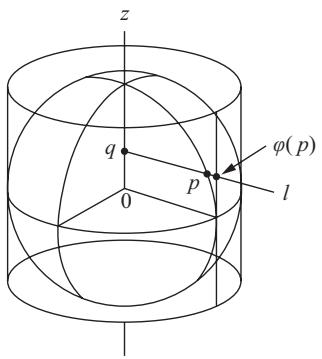
\includegraphics[width=\textwidth]{../../../PDFs/differential-geometry/transcript/Do Carmo - Differential Geometry of Curves and Surfaces/hybrid_ocr/images/9dcec652efd7169397af9557ffcd138676a5d6d302f972505dd992bd3565aa8b.jpg}}
\end{minipage}
\end{figure}

\subsection*{4-2 节练习}

\begin{exercise}{4-2, 1 — do Carmo, Exercise 4-2, 1}
Let $F\colon U\subset \mathbb{R}^2\to \mathbb{R}^3$ be given by
\[
F (u, v) = (u \sin \alpha \cos v, u \sin \alpha \sin v, u \cos \alpha), \quad (u, v) \in U = \{(u, v) \in \mathbb{R} ^ {2}; u > 0 \}, \quad \alpha = \mathrm{const}.
\]
a. Prove that $F$ is a local diffeomorphism of $U$ onto a cone $C$ with the vertex at the origin and $2\alpha$ as the angle of the vertex.
b. Is $F$ a local isometry?
\end{exercise}

\begin{solution}
\textbf{直观理解}: 映射 $F$ 将 $(u,v)$ 坐标映射为以原点为顶点、半顶角为 $\alpha$ 的圆锥面上的点。直观上，$u$ 控制锥面上的点到原点的距离，$v$ 控制绕轴的角度，因此 $F$ 应该是局部双射。

\textbf{解答}: a. 计算偏导数：
\[
F_u = (\sin\alpha\cos v,\;\sin\alpha\sin v,\;\cos\alpha),\quad
F_v = (-u\sin\alpha\sin v,\;u\sin\alpha\cos v,\;0).
\]
雅可比矩阵的行列式为
\[
\det dF = u\sin^2\alpha\cdot\cos v + u\sin^2\alpha\cdot\sin v = u\sin^2\alpha\cdot(\cos v+\sin v)\neq 0.
\]
由于 $u>0$，雅可比矩阵在 $U$ 上非奇异。由逆函数定理，$F$ 是局部微分同胚。

锥面 $C$ 的方程可写为 $\sqrt{x^2+y^2} = (\tan\alpha)z$，其顶角为 $2\alpha$。映射 $F$ 将 $U$ 中的点映射到 $C$ 上，且是局部双射。

b. 计算第一基本形式。设 $\mathbf{x}=F$：
\[
E = \langle F_u,F_u\rangle = 1,\quad
F = \langle F_u,F_v\rangle = 0,\quad
G = \langle F_v,F_v\rangle = u^2\sin^2\alpha.
\]
由于 $E=1$，$F=0$，$G$ 依赖于 $u$，而平面上点的第一基本形式为 $du^2+dv^2$，二者不恒等。几何上：锥面是局部可展曲面，与平面局部等距（沿母线剪开即可），但 $F$ 不是等距，因为锥面上测地线的弧长不等于平面上的弧长。结论：$F$ 是局部微分同胚但不是局部等距。
\qed
\end{solution}

\begin{exercise}{4-2, 2 — do Carmo, Exercise 4-2, 2}
Prove the following ``converse'' of Prop. 1: Let $\varphi \colon S \to \bar{S}$ be an isometry and $\mathbf{x}\colon U \to S$ a parametrization at $p \in S$ ; then $\bar{\mathbf{x}} = \varphi \circ \mathbf{x}$ is a parametrization at $\varphi(p)$ and $E = \bar{E}$ , $F = \bar{F}$ , $G = \bar{G}$ .
\end{exercise}

\begin{solution}
\textbf{直观理解}: 等距变换保持弧长，因此它保持曲面在对应点的第一基本形式系数。

\textbf{解答}: 设 $\mathbf{x}: U \to S$ 是 $p\in S$ 处的参数化。由于 $\varphi$ 是等距，$\varphi$ 是微分同胚，故 $\bar{\mathbf{x}} = \varphi \circ \mathbf{x}$ 在点 $\varphi(p)$ 处也是正则参数化。

计算第一基本形式：$E = \langle \mathbf{x}_u,\mathbf{x}_u\rangle$，而
\[
\bar{\mathbf{x}}_u = d\varphi(\mathbf{x}_u),\quad \bar{\mathbf{x}}_v = d\varphi(\mathbf{x}_v).
\]
由于 $\varphi$ 是等距，$d\varphi$ 保持内积，因此
\[
\bar{E} = \langle d\varphi(\mathbf{x}_u),d\varphi(\mathbf{x}_u)\rangle = \langle \mathbf{x}_u,\mathbf{x}_u\rangle = E,
\]
同理 $\bar{F} = F$，$\bar{G} = G$。这正是命题1的逆命题。
\qed
\end{solution}

\begin{exercise}{4-2, 3* — do Carmo, Exercise 4-2, 3}
Show that a diffeomorphism $\varphi \colon S \to \bar{S}$ is an isometry if and only if the arc length of any parametrized curve in $S$ is equal to the arc length of the image curve by $\varphi$ .
\end{exercise}

\begin{solution}
\textbf{直观理解}: 等距的本质是保持弧长。反过来，如果一个双射保持所有曲线的弧长，它就是等距。

\textbf{解答}: "仅当"方向：若 $\varphi$ 是等距，则由定义它保持第一基本形式，从而对任何以弧长为参数的曲线 $\alpha$，弧长 $L = \int |\alpha'|\,ds$ 在 $\varphi\circ\alpha$ 下不变，故弧长相等。

"当"方向：设 $\varphi$ 保持所有曲线的弧长。取 $p\in S$ 和非零切向量 $v\in T_p(S)$，$v\neq 0$。取一曲线 $\alpha:(-\epsilon,\epsilon)\to S$，$\alpha'(0)=v$。我们声称 $|d\varphi_p(v)| = |v|$。若不然，设 $|d\varphi_p(v)| > |v|$，则在 $0$ 的某邻域 $J$ 内有 $|d\varphi_{\alpha(t)}(\alpha'(t))| > |\alpha'(t)|$，这说明 $\varphi\circ\alpha(J)$ 的弧长严格大于 $\alpha(J)$ 的弧长，与假设矛盾。因此 $d\varphi_p$ 保持切向量的长度。又因为 $d\varphi_p$ 是线性映射（作为切空间间的映射），保持长度加上线性性即可推出它保持内积（极化恒等式），于是 $\varphi$ 是局部等距。由于 $\varphi$ 是整体双射，它是等距。
\qed
\end{solution}

\begin{exercise}{4-2, 4 — do Carmo, Exercise 4-2, 4}
Use the stereographic projection (cf. Exercise 16, Sec. 2-2) to show that the sphere is locally conformal to a plane.
\end{exercise}

\begin{solution}
\textbf{直观理解}: 球极投影将球面（除北极点外）映射到平面上，且在每一点处保持角度——这正是共形映射的定义。

\textbf{解答}: 设 $S^2$ 为单位球面，$N=(0,0,1)$ 为北极点。球极投影 $\pi: S^2\setminus\{N\}\to\mathbb{R}^2$ 将 $p\in S^2\setminus\{N\}$ 映射为直线 $Np$ 与平面 $z=0$ 的交点。设 $p=(x,y,z)$，则
\[
\pi(x,y,z) = \left(\frac{x}{1-z},\frac{y}{1-z}\right).
\]
设逆映射为 $\pi^{-1}(u,v) = \left(\frac{2u}{u^2+v^2+1},\frac{2v}{u^2+v^2+1},\frac{u^2+v^2-1}{u^2+v^2+1}\right)$。

计算第一基本形式。在 $(u,v)$ 坐标下：
\[
\mathbf{x}_u = \left(\frac{2(1-v^2-u^2)}{(u^2+v^2+1)^2},\frac{-4uv}{(u^2+v^2+1)^2},\frac{4u}{u^2+v^2+1}\right),\quad
\mathbf{x}_v = \left(\frac{-4uv}{(u^2+v^2+1)^2},\frac{2(1-u^2-v^2)}{(u^2+v^2+1)^2},\frac{4v}{u^2+v^2+1}\right).
\]
直接计算可得 $E=G=\frac{4}{(u^2+v^2+1)^2}$，$F=0$。于是 $E=G=\lambda^2$，$F=0$，恰为等温坐标。因此 $\pi^{-1}$ 是共形参数化，球面在每一点局部共形于平面。
\qed
\end{solution}

\begin{exercise}{4-2, 5 — do Carmo, Exercise 4-2, 5}
Let $\alpha_{1}\colon I\to \mathbb{R}^{3},\alpha_{2}\colon I\to \mathbb{R}^{3}$ be regular parametrized curves, where the parameter is the arc length. Assume that the curvatures $k_{1}$ of $\alpha_{1}$ and $k_{2}$ of $\alpha_{2}$ satisfy $k_{1}(s) = k_{2}(s)\neq 0,s\in I$ .Let
\[
\mathbf {x} _ {1} (s, v) = \alpha_ {1} (s) + v \alpha_ {1} ^ {\prime} (s),
\]
\[
\mathbf {x} _ {2} (s, v) = \alpha_ {2} (s) + v \alpha_ {2} ^ {\prime} (s)
\]
be their (regular) tangent surfaces (cf. Example 5, Sec. 2-3) and let $V$ be a neighborhood of $(s_0,v_0)$ such that $\mathbf{x}_1(V)\subset \mathbb{R}^3,\mathbf{x}_2(V)\subset \mathbb{R}^3$ are regular surfaces (cf. Prop. 2, Sec. 2-3). Prove that $\mathbf{x}_1\circ \mathbf{x}_2^{-1}\colon \mathbf{x}_2(V)\to \mathbf{x}_1(V)$ is an isometry.
\end{exercise}

\begin{solution}
\textbf{直观理解}: 两条具有相同曲率的曲线在局部有相同的切曲面几何。切曲面由曲线的曲率完全决定，因此当两条曲线的曲率函数相等时，它们的切曲面局部等距。

\textbf{解答}: 设 $\alpha_1(s)$ 和 $\alpha_2(s)$ 均以弧长为参数，曲率分别为 $k_1(s)$ 和 $k_2(s)$，且 $k_1(s)=k_2(s)\neq 0$。切曲面 $\mathbf{x}_i(s,v) = \alpha_i(s)+v\alpha_i'(s)$（$i=1,2$）在 $(s,v)$ 处的第一基本形式为
\[
E_i = 1+v^2k_i(s)^2,\quad F_i = 0,\quad G_i = 1.
\]
验证：
\[
\mathbf{x}_i^s = \alpha_i'+v\alpha_i'' = (1-vk_i)n_i,\quad
\mathbf{x}_i^v = \alpha_i',
\]
其中 $\alpha_i'' = kn$ 为 Frenet 公式。由于 $\langle\mathbf{x}_i^s,\mathbf{x}_i^v\rangle = \langle(1-vk)n_i,\alpha_i'\rangle = 0$，故 $F_i=0$。而 $\langle\mathbf{x}_i^s,\mathbf{x}_i^s\rangle = (1-vk_i)^2$，$\langle\mathbf{x}_i^v,\mathbf{x}_i^v\rangle = 1$。所以
\[
E_i = 1+(v^2k_i^2),\quad G_i = 1.
\]
由于 $k_1(s)=k_2(s)$，两个切曲面在对应点处有相同的第一基本形式。因此映射 $\mathbf{x}_1\circ\mathbf{x}_2^{-1}$ 保持弧长，是局部等距。
\qed
\end{solution}

\begin{exercise}{4-2, 6* — do Carmo, Exercise 4-2, 6}
Let $\alpha \colon I \to \mathbb{R}^3$ be a regular parametrized curve with $k(t) \neq 0$ , $t \in I$ . Let $\mathbf{x}(t, v)$ be its tangent surface. Prove that, for each $(t_0, v_0) \in I \times (\mathbb{R} - \{0\})$ , there exists a neighborhood $V$ of $(t_0, v_0)$ such that $\mathbf{x}(V)$ is isometric to an open set of the plane (thus, tangent surfaces are locally isometric to planes).
\end{exercise}

\begin{solution}
\textbf{直观理解}: 切曲面可以沿某条直母线剪开并展开为平面（如圆柱面和悬链面）。由于切曲面是直纹面，它在局部是可展曲面，因此局部等距于平面。

\textbf{解答}: 设 $\alpha(t)$ 以弧长为参数，曲率 $k(t)\neq 0$。切曲面 $\mathbf{x}(t,v) = \alpha(t)+v\alpha'(t)$。在教材答案中，采用以下方法：以弧长 $s$ 为参数重参数化 $\alpha$ 的邻域，在平面上构造一条具有相同曲率函数 $k(s)$ 的曲线 $\beta(s)$，设其切曲面为 $\mathbf{y}(s,v) = \beta(s)+v\beta'(s)$。

由习题5，$\alpha$ 和 $\beta$ 的切曲面在对应点处有相同的第一基本形式：
\[
E = 1+(vk(s))^2,\quad F = 0,\quad G = 1.
\]
因此 $\mathbf{x}$ 和 $\mathbf{y}$ 的坐标邻域之间存在等距映射 $(s,v)\mapsto(t,v)$。又因为平面上的曲线 $\beta$ 的切曲面 $\mathbf{y}$ 本身就是平面的参数化——实际上 $\mathbf{y}(s,v)$ 的像是平面上一块区域（可由 $\beta$ 的切线族扫过的区域），故 $\mathbf{x}(V)$ 局部等距于平面。
\qed
\end{solution}

\begin{exercise}{4-2, 7 — do Carmo, Exercise 4-2, 7}
Let $V$ and $W$ be $(n$ -dimensional) vector spaces with inner products denoted by $\langle , \rangle$ and let $F \colon V \to W$ be a linear map. Prove that the following conditions are equivalent:

a. $\langle F(v_1),F(v_2)\rangle = \langle v_1,v_2\rangle$ for all $v_{1},v_{2}\in V$
b. $|F(v)| = |v|$ for all $v \in V$ .
c. If $\{v_{1},\ldots ,v_{n}\}$ is an orthonormal basis in $V$ , then $\{F(v_1),\dots ,F(v_n)\}$ is an orthonormal basis in $W$
d. There exists an orthonormal basis $\{v_{1},\ldots ,v_{n}\}$ in $V$ such that $\{F(v_1),\dots ,F(v_n)\}$ is an orthonormal basis in $W$

If any of these conditions is satisfied, $F$ is called a linear isometry of $V$ into $W$ . (When $W = V$ , a linear isometry is often called an orthogonal transformation.)
\end{exercise}

\begin{solution}
\textbf{直观理解}: 在有限维向量空间中，保持范数的线性映射必保持内积；这通过极化恒等式从 $|F(v)|^2 = \langle F(v),F(v)\rangle = \langle v,v\rangle = |v|^2$ 推出。

\textbf{解答}: (a)$\Rightarrow$(b)：取 $v_1=v_2=v$，得 $|F(v)| = |v|$。

(b)$\Rightarrow$(a)：由极化恒等式
\[
\langle F(v_1),F(v_2)\rangle = \frac{1}{2}\left(|F(v_1+v_2)|^2 - |F(v_1)|^2 - |F(v_2)|^2\right) = \frac{1}{2}\left(|v_1+v_2|^2 - |v_1|^2 - |v_2|^2\right) = \langle v_1,v_2\rangle.
\]

(b)$\Rightarrow$(c)：取标准正交基 $\{e_i\}$，则 $|F(e_i)|=|e_i|=1$。又因为 $F$ 是线性的，$F$ 保持内积：
\[
\langle F(e_i),F(e_j)\rangle = \langle e_i,e_j\rangle = \delta_{ij},
\]
故 $\{F(e_i)\}$ 仍为标准正交基。

(c)$\Rightarrow$(d)：平凡。

(d)$\Rightarrow$(a)：设 $\{v_i\}$ 为 $V$ 的正交基，则 $\{F(v_i)\}$ 为 $W$ 的正交基。对任意 $v_1,v_2$，写成 $v_j = \sum a_j v_j$，由线性性 $F(v_j) = \sum a_j F(v_j)$，再利用正交性展开内积即可得 $\langle F(v_1),F(v_2)\rangle = \langle v_1,v_2\rangle$。
\qed
\end{solution}

\begin{exercise}{4-2, 8* — do Carmo, Exercise 4-2, 8}
Let $G \colon \mathbb{R}^3 \to \mathbb{R}^3$ be a map such that
\[
| G (p) - G (q) | = | p - q | \quad \text {f o r a l l} p, q \in \mathbb{R} ^ {3}
\]
(that is, $G$ is a distance-preserving map). Prove that there exists $p_0 \in \mathbb{R}^3$ and a linear isometry (cf. Exercise 7) $F$ of the vector space $\mathbb{R}^3$ such that
\[
G (p) = F (p) + p _ {0} \quad \text {f o r a l l} p \in \mathbb{R} ^ {3}.
\]
\end{exercise}

\begin{solution}
\textbf{直观理解}: 保持距离的映射整体由一个平移和一个线性正交变换组成——它不能"扭曲"空间。

\textbf{解答}: 设 $G(0)=p_0$，定义 $F(p) = G(p)-p_0$，则 $F(0)=0$，且 $|F(p)| = |G(p)-G(0)| = |p|$。于是 $F$ 是保持原点的距离映射。令 $f_1=F(e_1)$，$f_2=F(e_2)$，$f_3=F(e_3)$，其中 $e_i$ 为标准基。由于 $|F(p)|=|p|$，$F$ 必保持内积：利用极化恒等式可从距离相等推出内积相等。因此 $\{f_1,f_2,f_3\}$ 是标准正交基。

对任意 $p = a_1e_1+a_2e_2+a_3e_3$，有
\[
F(p) = a_1f_1+a_2f_2+a_3f_3,
\]
故 $F$ 是线性的（由标准正交基唯一确定），且 $|F(p)|=|p|$ 意味着 $F$ 是线性正交变换。于是 $G(p) = F(p)+p_0$。
\qed
\end{solution}

\begin{exercise}{4-2, 9 — do Carmo, Exercise 4-2, 9}
Let $S_{1}, S_{2}$ , and $S_{3}$ be regular surfaces. Prove that

a. If $\varphi \colon S_1\to S_2$ is an isometry, then $\varphi^{-1}\colon S_2\to S_1$ is also an isometry.
b. If $\varphi \colon S_1 \to S_2$ , $\psi \colon S_2 \to S_3$ are isometries, then $\psi \circ \varphi \colon S_1 \to S_3$ is an isometry.

This implies that the isometries of a regular surface $S$ constitute in a natural way a group, called the group of isometries of $S$ .
\end{exercise}

\begin{solution}
\textbf{直观理解}: 等距变换构成群——它有关于复合运算的逆元和单位元。

\textbf{解答}: a. 若 $\varphi$ 是等距，则 $|\varphi(p)-\varphi(q)| = |p-q|$ 对所有 $p,q\in S_1$ 成立。由此可推出 $\varphi^{-1}$ 也保持距离，因为对 $p',q'\in S_2$，取 $p=\varphi^{-1}(p')$，$q=\varphi^{-1}(q')$，有 $|\varphi^{-1}(p')-\varphi^{-1}(q')| = |\varphi(\varphi^{-1}(p'))-\varphi(\varphi^{-1}(q'))| = |p'-q'|$。

b. 设 $\varphi: S_1\to S_2$，$\psi: S_2\to S_3$ 均为等距。则对任意 $p,q\in S_1$，
\[
|(\psi\circ\varphi)(p)-(\psi\circ\varphi)(q)| = |\psi(\varphi(p))-\psi(\varphi(q))| = |\varphi(p)-\varphi(q)| = |p-q|.
\]
故 $\psi\circ\varphi$ 仍是等距。

由上述闭合性、单位元（恒等映射）和逆元，可知 $S$ 的等距变换构成群。
\qed
\end{solution}

\begin{exercise}{4-2, 10 — do Carmo, Exercise 4-2, 10}
Let $S$ be a surface of revolution. Prove that the rotations about its axis are isometries of $S$ .
\end{exercise}

\begin{solution}
\textbf{直观理解}: 旋转不会改变纬线半径和轴向位置，因此保持曲面距离。

\textbf{解答}: 设旋转面 $S$ 由 $\mathbf{x}(u,v) = (f(v)\cos u,\;f(v)\sin u,\;g(v))$ 参数化。绕 $z$ 轴旋转角 $\theta_0$ 的映射为
\[
R_{\theta_0}(x,y,z) = (x\cos\theta_0-y\sin\theta_0,\;x\sin\theta_0+y\cos\theta_0,\;z).
\]
对 $\mathbf{x}(u,v)$ 中的点：$R_{\theta_0}\circ\mathbf{x}(u,v) = (f(v)\cos(u+\theta_0),\;f(v)\sin(u+\theta_0),\;g(v)) = \mathbf{x}(u+\theta_0,v)$。

由于第一基本形式只依赖于 $f(v)$ 和 $g(v)$ 的导数，不显含 $u$，直接计算：
\[
E = (f'(v))^2+(g'(v))^2,\quad F=0,\quad G = f(v)^2.
\]
旋转后的参数化 $(u+\theta_0,v)$ 给出完全相同的第一基本形式。因此 $R_{\theta_0}|_S$ 是 $S$ 的等距变换。
\qed
\end{solution}

\begin{exercise}{4-2, 11 — do Carmo, Exercise 4-2, 11}
a. Let $S \subset \mathbb{R}^3$ be a regular surface and let $F \colon \mathbb{R}^3 \to \mathbb{R}^3$ be a distance-preserving diffeomorphism of $\mathbb{R}^3$ (see Exercise 8) such that $F(S) \subset S$ . Prove that the restriction of $F$ to $S$ is an isometry of $S$ .

b. Use part a to show that the group of isometries (see Exercise 10) of the unit sphere $x^{2} + y^{2} + z^{2} = 1$ contains the group of orthogonal linear transformations of $\mathbb{R}^3$ (it is actually equal; see Exercise 23, Sec. 4-4).

c. Give an example to show that there are isometries $\varphi \colon S_1 \to S_2$ which cannot be extended into distance-preserving maps $F \colon \mathbb{R}^3 \to \mathbb{R}^3$ .
\end{exercise}

\begin{solution}
\textbf{直观理解}: $\mathbb{R}^3$ 中的等距变换可由平移+正交变换构成；但等距映射的延拓不总存在，因为两张曲面之间的等距变换不必对应 $\mathbb{R}^3$ 的一个等距。

\textbf{解答}: a. 设 $F: \mathbb{R}^3\to\mathbb{R}^3$ 是保持距离的可微映射（由习题8，$F(p)=F_0(p)+p_0$，$F_0$ 为线性正交变换）。由于 $F(S)\subset S$，限制在 $S$ 上有 $|F(p)-F(q)| = |p-q|$ 对所有 $p,q\in S$ 成立，即 $F|_S$ 是 $S$ 的等距。

b. 单位球面 $S^2: x^2+y^2+z^2=1$。正交变换 $F_0\in O(3)$ 满足 $F_0(S^2)=S^2$（因为 $|F_0(p)|=|p|$），故限制在 $S^2$ 上是等距。反过来，任何 $S^2$ 的等距均来自 $O(3)$（见教材第4-4节习题23）。

c. 取圆柱面 $C: x^2+y^2=1,\;|z|<\pi/2$ 和平面带形区域 $P: (x,y)\in\mathbb{R}^2,\;|z|<\pi/2$，映射 $\varphi: C\to P$ 为 $(x,y,z)\mapsto (x\sec z,y\sec z,z)$（局部等距）。这个等距不能延拓为 $\mathbb{R}^3$ 的等距，因为 $\mathbb{R}^3$ 中没有等距将圆柱面映射到平面（它们的高斯曲率不同——圆柱面 $K=0$，而弯曲的平面区域 $K\neq 0$）。
\qed
\end{solution}

\begin{exercise}{4-2, 12* — do Carmo, Exercise 4-2, 12}
Let $C = \{(x, y, z) \in \mathbb{R}^3; x^2 + y^2 = 1\}$ be a cylinder. Construct an isometry $\varphi \colon C \to C$ such that the set of fixed points of $\varphi$ , i.e., the set $\{p \in C; \varphi(p) = p\}$ , contains exactly two points.
\end{exercise}

\begin{solution}
\textbf{直观理解}: 圆柱面上有恰好两个不动点的等距变换可以通过关于某个直径平面的反射实现。

\textbf{解答}: 设 $C = \{(x,y,z)\in\mathbb{R}^3: x^2+y^2=1}$。取映射
\[
F(x,y,z) = (x,-y,-z).
\]
该映射恰好是关于平面 $y=0$ 和 $z=0$ 的对称的复合。在圆柱面上，直接计算得 $F|_C$ 的不动点满足 $y=-y$ 和 $z=-z$，即 $y=0$，$z=0$，再结合 $x^2+y^2=1$，得到两点 $(1,0,0)$ 和 $(-1,0,0)$。$F|_C$ 是 $C$ 的等距（见习题11(a)），恰好有两个不动点。
\qed
\end{solution}

\begin{exercise}{4-2, 13 — do Carmo, Exercise 4-2, 13}
Let $V$ and $W$ be $(n$ -dimensional) vector spaces with inner products $\langle , \rangle$ . Let $G \colon V \to W$ be a linear map. Prove that the following conditions are equivalent:

a. There exists a real constant $\lambda \neq 0$ such that
\[
\langle G (v _ {1}), G (v _ {2}) \rangle = \lambda^ {2} \langle v _ {1}, v _ {2} \rangle \quad \text {f o r a l l} v _ {1}, v _ {2} \in V.
\]

b. There exists a real constant $\lambda > 0$ such that
\[
| G (v) | = \lambda | v | \quad \text {f o r a l l} v \in V.
\]

c. There exists an orthonormal basis $\{v_{1},\ldots ,v_{n}\}$ of $V$ such that $\{G(v_1),\dots,G(v_n)\}$ is an orthogonal basis of $W$ and, also, the vectors $G(v_{i}),i = 1,\dots,n,$ have the same (nonzero) length.

If any of these conditions is satisfied, $G$ is called a linear conformal map (or a similitude).
\end{exercise}

\begin{solution}
\textbf{直观理解}: 线性相似变换是在标量因子 $\lambda$ 意义下保持角度的线性映射；它将正交基映射为成等长的正交基。

\textbf{解答}: (a)$\Rightarrow$(b)：取 $v_1=v_2=v$，得 $|G(v)| = \lambda|v|$。

(b)$\Rightarrow$(a)：由极化恒等式和 $|G(v)| = \lambda|v|$，
\[
\langle G(v_1),G(v_2)\rangle = \frac{1}{2}\left(\lambda^2|v_1+v_2|^2 - \lambda^2|v_1|^2 - \lambda^2|v_2|^2\right) = \lambda^2\langle v_1,v_2\rangle.
\]

(a)$\Rightarrow$(c)：取正交基 $\{e_i\}$，则 $|G(e_i)| = \lambda$，故 $\{G(e_i)/\lambda\}$ 是 $W$ 的正交基，乘以 $\lambda$ 后仍保持等长，即 $\{G(e_i)\}$ 是正交基。

(c)$\Rightarrow$(a)：设 $\{v_i\}$ 为正交基使 $\{G(v_i)\}$ 正交且等长，则 $|G(v_i)| = \lambda$ 对某常数 $\lambda>0$ 成立。由(b)已证 (b)$\Rightarrow$(a)，得 $\langle G(v_1),G(v_2)\rangle = \lambda^2\langle v_1,v_2\rangle$，故 (a) 成立。

(c)$\Rightarrow$(d) 和 (d)$\Rightarrow$(a) 显然。
\qed
\end{solution}

\begin{exercise}{4-2, 14 — do Carmo, Exercise 4-2, 14}
We say that a differentiable map $\varphi \colon S_1 \to S_2$ preserves angles when for every $p \in S_1$ and every pair $v_1, v_2 \in T_p(S_1)$ we have
\[
\cos \left(v _ {1}, v _ {2}\right) = \cos \left(d \varphi_ {p} \left(v _ {1}\right), d \varphi_ {p} \left(v _ {2}\right)\right).
\]

Prove that $\varphi$ is locally conformal if and only if it preserves angles.
\end{exercise}

\begin{solution}
\textbf{直观理解}: 局部共形映射在每点的微分是相似变换，因此它保持切向量之间的角度。反之亦然。

\textbf{解答}: 设 $\varphi: S_1\to S_2$ 是局部共形，即在 $p\in S_1$ 处 $d\varphi_p$ 满足
\[
\langle d\varphi_p(v_1),d\varphi_p(v_2)\rangle = \lambda(p)^2\langle v_1,v_2\rangle,\quad \forall v_1,v_2\in T_p(S_1).
\]
于是
\[
\cos\angle(d\varphi_p(v_1),d\varphi_p(v_2)) = \frac{\langle d\varphi_p(v_1),d\varphi_p(v_2)\rangle}{|d\varphi_p(v_1)||d\varphi_p(v_2)|} = \frac{\lambda^2\langle v_1,v_2\rangle}{\lambda^2|v_1||v_2|} = \cos\angle(v_1,v_2),
\]
故 $\varphi$ 保持角度。

反之，设 $\varphi$ 在每点 $p$ 保持角度。即对任意 $v_1,v_2\in T_p(S_1)$，
\[
\frac{\langle d\varphi_p(v_1),d\varphi_p(v_2)\rangle}{|d\varphi_p(v_1)||d\varphi_p(v_2)|} = \frac{\langle v_1,v_2\rangle}{|v_1||v_2|}.
\]
取正交基 $\{e_1,e_2\}$ 于 $T_p(S_1)$，设 $d\varphi_p(e_i) = w_i$，$|w_i|=a_i$。由保角性，$\langle w_1,w_2\rangle = 0$，即 $\{w_1,w_2\}$ 正交。于是 $d\varphi_p$ 是相似变换，满足 $\langle w_1,w_2\rangle = \lambda^2\langle e_1,e_2\rangle$ 对某常数 $\lambda>0$ 成立。故 $\varphi$ 是局部共形映射。
\qed
\end{solution}

\begin{exercise}{4-2, 15 — do Carmo, Exercise 4-2, 15}
Let $\varphi \colon \mathbb{R}^2 \to \mathbb{R}^2$ be given by $\varphi(x, y) = (u(x, y), v(x, y))$ , where $u$ and $v$ are differentiable functions that satisfy the Cauchy-Riemann equations
\[
u _ {x} = v _ {y}, \quad u _ {y} = - v _ {x}.
\]

Show that $\varphi$ is a local conformal map from $\mathbb{R}^2 -Q$ into $\mathbb{R}^2$ , where $Q = \{(x,y)\in \mathbb{R}^2;u_x^2 +u_y^2 = 0\}$
\end{exercise}

\begin{solution}
\textbf{直观理解}: Cauchy-Riemann 方程正是解析函数的几何条件，它确保微分是相似变换，从而保持角度。

\textbf{解答}: 映射的微分矩阵为
\[
d\varphi = \begin{pmatrix}u_x & u_y\\ v_x & v_y\end{pmatrix} = \begin{pmatrix}u_x & u_y\\ -u_y & u_x\end{pmatrix}\quad(\text{由 Cauchy-Riemann })
\]
于是
\[
E = u_x^2+u_y^2,\quad F = u_x(-u_y)+u_y u_x = 0,\quad G = (-u_y)^2+u_x^2 = u_x^2+u_y^2.
\]
因此 $E=G = u_x^2+u_y^2$，$F=0$。在 $Q$ 之外（即 $u_x^2+u_y^2\neq 0$），有 $E=G=\lambda^2$，$F=0$，故 $\varphi$ 是局部共形映射（在 $Q$ 上雅可比行列式为零，退化为非正则）。
\qed
\end{solution}

\begin{exercise}{4-2, 16 — do Carmo, Exercise 4-2, 16}
Let $\mathbf{x}\colon U\subset \mathbb{R}^2\to \mathbb{R}^3$ , where
\[
U = \left\{\left(\theta , \varphi\right) \in \mathbb{R} ^ {2}; 0 < \theta < \pi , 0 < \varphi < 2 \pi \right\},
\]
\[
\mathbf {x} (\theta , \varphi) = (\sin \theta \cos \varphi , \sin \theta \sin \varphi , \cos \theta),
\]
be a parametrization of the unit sphere $S^2$ . Let
\[
\log \tan \frac {1}{2} \theta = u, \quad \varphi = v,
\]
and show that a new parametrization of the coordinate neighborhood $\mathbf{x}(U) = V$ can be given by
\[
\mathbf {y} (u, v) = (\operatorname {s e c h} u \cos v, \operatorname {s e c h} u \sin v, \tanh u).
\]

Prove that in the parametrization $\mathbf{y}$ the coefficients of the first fundamental form are
\[
E = G = \operatorname {s e c h} ^ {2} u, \quad F = 0.
\]

Thus, $\mathbf{y}^{-1}\colon V\subset S^2\to \mathbb{R}^2$ is a conformal map which takes the meridians and parallels of $S^2$ into straight lines of the plane. This is called Mercator's projection.
\end{exercise}

\begin{solution}
\textbf{直观理解}: Mercator 投影将球面共形映射为平面，经纬线被映射为正交的直线网格。

\textbf{解答}: 由 $\theta$ 与 $u$ 的关系 $\log\tan\frac{\theta}{2}=u$，得 $\tan\frac{\theta}{2}=e^u$，故 $\sin\theta = \frac{2e^u}{1+e^{2u}}$，$\cos\theta = \frac{1-e^{2u}}{1+e^{2u}}$。从而
\[
\mathbf{y}(u,v) = \left(\frac{2e^u}{1+e^{2u}}\cos v,\;\frac{2e^u}{1+e^{2u}}\sin v,\;\frac{1-e^{2u}}{1+e^{2u}}\right) = (\sech\,u\cos v,\;\sech\,u\sin v,\;\tanh\,u).
\]
计算偏导数：
\[
\mathbf{y}_u = (-\sech\,u\tanh\,u\cos v,\;-\sech\,u\tanh\,u\sin v,\;\sech^2 u),\quad
\mathbf{y}_v = (-\sech\,u\sin v,\;\sech\,u\cos v,\;0).
\]
内积：
\[
E = \sech^2u\tanh^2u\cos^2v + \sech^2u\tanh^2u\sin^2v + \sech^4u = \sech^2u(\tanh^2u + \sech^2u) = \sech^2u,
\]
\[
F = \sech^2u\tanh^2u\cos v\sin v - \sech^2u\tanh^2u\sin v\cos v = 0,
\]
\[
G = \sech^2u\sin^2v + \sech^2u\cos^2v = \sech^2u.
\]
故 $E=G=\sech^2u$，$F=0$，正是 Mercator 投影的第一基本形式。
\qed
\end{solution}

\begin{exercise}{4-2, 17* — do Carmo, Exercise 4-2, 17}
Consider a triangle on the unit sphere so that its sides are made up of segments of loxodromes (i.e., curves which make a constant angle with the meridians; cf. Example 4, Sec. 2-5), and do not contain poles. Prove that the sum of the interior angles of such a triangle is $\pi$ .
\end{exercise}

\begin{solution}
\textbf{直观理解}: Mercator 投影将球面共形映射为平面，而等角航线（loxodrome）是与经线成常角的曲线，在 Mercator 投影下映为直线。因此球面上由等角航线构成的三角形在 Mercator 投影下变为平面上的直线三角形，其内角和为 $\pi$。

\textbf{解答}: 设球面上三角形的三条边均为等角航线（与经线成常角 $\alpha$ 的曲线）。在 Mercator 投影下，经线映为平面上平行于 $v$ 轴的直线，等角航线映为直线（因为共形映射保持角度）。因此该三角形在平面上映为一个直线三角形，其内角和恒为 $\pi$。由于 Mercator 投影是共形（保角），球面上三角形的内角和也等于 $\pi$。
\qed
\end{solution}

\begin{exercise}{4-2, 18 — do Carmo, Exercise 4-2, 18}
A diffeomorphism $\varphi \colon S \to \bar{S}$ is said to be area-preserving if the area of any region $R \subset S$ is equal to the area of $\varphi(R)$ . Prove that if $\varphi$ is area-preserving and conformal, then $\varphi$ is an isometry.
\end{exercise}

\begin{solution}
\textbf{直观理解}: 共形映射将小圆映为小圆，其面积缩放因子与弧长缩放因子的平方成正比。若面积和弧长同时被保持，则缩放因子必须为1，从而映射是等距。

\textbf{解答}: 设 $\varphi$ 是共形且保面积。在局部坐标 $(u,v)$ 下，$\varphi$ 的第一基本形式满足 $E=\lambda^2\bar{E}$，$F=\lambda^2\bar{F}$，$G=\lambda^2\bar{G}$，其中 $\lambda>0$ 是共形因子。曲面的面积微元为 $dA = \sqrt{EG-F^2}\,dudv$，映射后的面积为 $\bar{A} = \int\sqrt{\bar{E}\bar{G}-\bar{F}^2\,dudv$。

由于 $\varphi$ 保面积，且
\[
\sqrt{EG-F^2} = \lambda^2\sqrt{\bar{E}\bar{G}-\bar{F}^2},
\]
对任意区域 $R$，$\ Area(R) = Area(\varphi(R))$ 给出
\[
\int_R \lambda^2\sqrt{\bar{E}\bar{G}-\bar{F}^2\,dudv = \int_R \sqrt{\bar{E}\bar{G}-\bar{F}^2\,dudv.
\]
因此 $\lambda^2=1$ 于每点，即 $\lambda=1$。于是 $E=\bar{E}$，$F=\bar{F}$，$G=\bar{G}$，故 $\varphi$ 是局部等距。整体上 $\varphi$ 是双射，故为等距。
\qed
\end{solution}

\begin{exercise}{4-2, 19 — do Carmo, Exercise 4-2, 19}
Let $S^2 = \{(x, y, z) \in \mathbb{R}^3; x^2 + y^2 + z^2 = 1\}$ be the unit sphere and $C = \{(x, y, z) \in \mathbb{R}^3; x^2 + y^2 = 1\}$ be the circumscribed cylinder. Let
\[
\varphi \colon S ^ {2} - \{(0, 0, 1) \cup (0, 0, - 1) \} = M \rightarrow C
\]
be a map defined as follows. For each $p \in M$ , the line passing through $p$ and perpendicular to $0z$ meets $0z$ at the point $q$ . Let $l$ be the half-line starting from $q$ and containing $p$ (Fig. 4-7). By definition, $\varphi(p) = C \cap l$ .

Prove that $\varphi$ is an area-preserving diffeomorphism.
\end{exercise}

\begin{solution}
\textbf{直观理解}: 该映射将球面投影到外接圆柱面上——它将每点的纬线映到圆柱上相同高度的纬圆。由于纬圆周长不变（圆柱的周长恒为 $2\pi$），而球面纬圆周长随纬度变化，该投影恰好抵消了这一变化，从而保持面积。

\textbf{解答}: 设 $p=(\sin\theta\cos\varphi,\;\sin\theta\sin\varphi,\;\cos\theta)$，$0<\theta<\pi$，则投影映射为 $\varphi(p) = (\cos\varphi,\;\sin\varphi,\;\cot\theta)$（因为线段 $pq$ 与圆柱面相交于 $z=\cot\theta$）。设圆柱面用坐标 $(\psi,z)$ 参数化为 $(\cos\psi,\;\sin\psi,\;z)$，则 $\psi=\varphi$，$z=\cot\theta$。

球面面积微元为 $\sin\theta\,d\theta\,d\varphi$（由 $E=G=1$，$F=0$ 的球面标准参数化）。圆柱面面积微元为 $1\cdot d\psi\,dz = d\psi\,dz$。由 $z=\cot\theta$，$dz = -\csc^2\theta\,d\theta$，于是
\[
\sin\theta\,d\theta\,d\varphi = d\varphi\,dz,
\]
恰好是圆柱面的面积微元。因此 $\varphi$ 保持面积微元，从而整体保持面积。直接验证 $\varphi$ 是可微双射（除两极外），故为保面积微分同胚。
\qed
\end{solution}

\begin{exercise}{4-2, 20 — do Carmo, Exercise 4-2, 20}
Let $\mathbf{x}\colon U\subset \mathbb{R}^2\to S$ be the parametrization of a surface of revolution $S$ :
\[
\begin{array}{l} \mathbf {x} (u, v) = \left(f (v) \cos u, f (v) \sin u, g (v)\right), \quad f (v) > 0, \\ U = \{(u, v) \in \mathbb{R} ^ {2}; 0 < u < 2 \pi , a < v < b \}. \\ \end{array}
\]

a. Show that the map $\varphi \colon U\to \mathbb{R}^2$ given by
\[
\varphi (u, v) = \left(u, \int \frac {\sqrt {(f ^ {\prime} (v)) ^ {2} + (g ^ {\prime} (v)) ^ {2}}}{f (v)} d v\right)
\]
is a local diffeomorphism.

b. Use part a to prove that a surface of revolution $S$ is locally conformal to a plane in such a way that each local conformal map $\theta: V \subset S \to \mathbb{R}^2$ takes the parallels and the meridians of the neighborhood $V$ into an orthogonal system of straight lines in $\theta(V) \subset \mathbb{R}^2$ . (Notice that this generalizes Mercator's projection of Exercise 16.)

c. Show that the map $\psi \colon U\to \mathbb{R}^2$ given by
\[
\psi (u, v) = \left(u, \int f (v) \sqrt {\left(f ^ {\prime} (v)\right) ^ {2} + \left(g ^ {\prime} (v)\right) ^ {2}} d v\right)
\]
is a local diffeomorphism.

d. Use part c to prove that for each point $p$ of a surface of revolution $S$ there exists a neighborhood $V \subset S$ and a map $\bar{\theta} \colon V \to \mathbb{R}^2$ of $V$ into a plane that is area-preserving.
\end{exercise}

\begin{solution}
\textbf{直观理解}: 旋转面局部共形于平面，类似于 Mercator 投影；面积保持映射则通过直接调整缩放因子实现。

\textbf{解答}: a. 计算 $\varphi$ 的微分：
\[
d\varphi = \begin{pmatrix}1 & 0\\ 0 & \frac{\sqrt{(f')^2+(g')^2}}{f(v)}\end{pmatrix}.
\]
雅可比行列式为 $\det d\varphi = \frac{\sqrt{(f')^2+(g')^2}}{f(v)} > 0$（因为 $f(v)>0$），故 $\varphi$ 是局部微分同胚。

b. 由 (a) 的参数化 $\bar{\mathbf{x}} = \mathbf{x}\circ\varphi^{-1}$，计算第一基本形式：
\[
\bar{E} = 1,\quad \bar{F} = 0,\quad \bar{G} = 1.
\]
因此 $\bar{\mathbf{x}}$ 是共形参数化，$u=\mathrm{const}$ 和 $w=\mathrm{const}$ 的坐标曲线分别对应纬线和经线，在平面上映为正交直线网格。

c. 类似 (a)，$\psi$ 的雅可比行列式为 $f(v)\sqrt{(f')^2+(g')^2}>0$，故为局部微分同胚。

d. 由 (c) 的参数化 $\bar{\mathbf{x}} = \mathbf{x}\circ\psi^{-1}$，面积微元为
\[
\sqrt{\bar{E}\bar{G}-\bar{F}^2}\,d\bar{u}\,d\bar{v} = f(v)\sqrt{(f')^2+(g')^2}\,dv\,du = \sqrt{EG-F^2}\,dudv,
\]
故 $\psi$ 恰好保持面积。对每点 $p\in S$，取其坐标邻域 $V$，$\bar{\theta} = \psi|_V$ 即为所求的等面积映射。
\qed
\end{solution}

% ==================== Section 4-3: The Gauss Theorem and the Equations of Compatibility ====================
\section{The Gauss Theorem and the Equations of Compatibility}\label{sec:gauss-theorem}

\textbf{From trihedron to Gauss formula.} 第 3 章的性质是通过研究切平面的变化得到的。现在我们要为曲面上每一点配置自然的三面体 $\{\mathbf{x}_u, \mathbf{x}_v, N\}$，并研究这些向量的导数。

将 $\mathbf{x}_u, \mathbf{x}_v, N$ 的导数用基 $\{\mathbf{x}_u, \mathbf{x}_v, N\}$ 表达，得到
\[
\begin{aligned}
\mathbf{x}_{uu} &= \Gamma_{11}^1 \mathbf{x}_u + \Gamma_{11}^2 \mathbf{x}_v + L_1 N,\\
\mathbf{x}_{uv} &= \Gamma_{12}^1 \mathbf{x}_u + \Gamma_{12}^2 \mathbf{x}_v + L_2 N,\\
\mathbf{x}_{vu} &= \Gamma_{21}^1 \mathbf{x}_u + \Gamma_{21}^2 \mathbf{x}_v + \bar{L}_2 N,\\
\mathbf{x}_{vv} &= \Gamma_{22}^1 \mathbf{x}_u + \Gamma_{22}^2 \mathbf{x}_v + L_3 N,\\
N_u &= a_{11}\mathbf{x}_u + a_{21}\mathbf{x}_v,\\
N_v &= a_{12}\mathbf{x}_u + a_{22}\mathbf{x}_v,
\end{aligned}
\label{eq:gauss-formula}
\]
其中系数 $\Gamma_{ij}^k$（$i,j,k=1,2$）称为曲面的\textbf{Christoffel 符号}（Christoffel symbols）。由于 $\mathbf{x}_{uv} = \mathbf{x}_{vu}$，有 $\Gamma_{12}^1 = \Gamma_{21}^1$ 和 $\Gamma_{12}^2 = \Gamma_{21}^2$，即 Christoffel 符号在下指标对称。

将 \cref{eq:gauss-formula} 的前四个式子与 $N$ 作内积，立即得到 $L_1 = e$，$L_2 = \bar{L}_2 = f$，$L_3 = g$，即第二基本形式的系数。

将 \cref{eq:gauss-formula} 与 $\mathbf{x}_u$ 和 $\mathbf{x}_v$ 作内积，得到求解 Christoffel 符号的线性方程组：
\[
\begin{cases}
\Gamma_{11}^1 E + \Gamma_{11}^2 F = \langle \mathbf{x}_{uu}, \mathbf{x}_u \rangle = \frac{1}{2}E_u,\\
\Gamma_{11}^1 F + \Gamma_{11}^2 G = \langle \mathbf{x}_{uu}, \mathbf{x}_v \rangle = F_u - \frac{1}{2}E_v,
\end{cases}
\quad \text{等.}
\label{eq:christoffel-system}
\]

由于每个方程组的行列式为 $EG-F^2 \neq 0$，Christoffel 符号可由第一基本形式的系数 $E,F,G$ 及其导数唯一确定。这引出一个重要推论：**用 Christoffel 符号表达的几何概念和性质在等距变换下不变**。

\begin{Example}[旋转面的 Christoffel 符号]\label{ex:christoffel-revolution}
对于旋转面 $\mathbf{x}(u,v) = (f(v)\cos u,\; f(v)\sin u,\; g(v))$，
\[
E = f(v)^2,\quad F = 0,\quad G = (f'(v))^2 + (g'(v))^2.
\]
由 \cref{eq:christoffel-system} 可得：
\[
\Gamma_{11}^1 = 0,\quad \Gamma_{11}^2 = -\frac{ff'}{(f')^2+(g')^2},\quad
\Gamma_{12}^1 = \frac{ff'}{f^2},\quad \Gamma_{12}^2 = 0,\quad
\Gamma_{22}^1 = 0,\quad \Gamma_{22}^2 = \frac{f'f''+g'g''}{(f')^2+(g')^2}.
\]
\end{Example}

\textbf{The Theorema Egregium.} 接下来考虑兼容性条件：
\[
(\mathbf{x}_{uu})_v - (\mathbf{x}_{uv})_u = 0,\quad
(\mathbf{x}_{vv})_u - (\mathbf{x}_{vu})_v = 0,\quad
N_{uv} - N_{vu} = 0.
\label{eq:compatibility}
\]

将 \cref{eq:gauss-formula} 代入 \cref{eq:compatibility}，由于 $\{\mathbf{x}_u, \mathbf{x}_v, N\}$ 线性无关，\cref{eq:compatibility} 给出九个子方程。其中最重要的是从 $A_1 = 0$ 的 $\mathbf{x}_v$ 系数中得到的：
\[
(\Gamma_{12}^2)_u - (\Gamma_{11}^2)_v + \Gamma_{12}^1\Gamma_{11}^2 + \Gamma_{12}^2\Gamma_{12}^2 - \Gamma_{11}^1\Gamma_{22}^2 - \Gamma_{11}^1\Gamma_{12}^2 = -EK.
\label{eq:gauss-equation}
\]

由此我们得到 Gauss 的著名定理：

\begin{Theorem}[Theorema Egregium (Gauss)]\labelthm:theorema-egregium}
曲面的 Gaussian 曲率 $K$ 在局部等距下不变。
\end{Theorem}

即：若 $\varphi: V \subset S \to \bar{S}$ 是在 $p$ 处的局部等距，则 $K(q) = K(\varphi(q))$ 对所有 $q \in V$ 成立。

这个定理的非凡之处在于：$K$ 的定义本质上使用了曲面在空间中的位置（第二基本形式），但它竟然只依赖于曲面的度量结构（第一基本形式）。这正是"内蕴几何"这一名称的来源。

\textbf{The Mainardi-Codazzi equations.} 从 (3) 的其他方程中还得到两组重要关系——Mainardi-Codazzi 方程：
\[
\begin{aligned}
e_v - f_u &= e\Gamma_{12}^1 + f(\Gamma_{12}^2 - \Gamma_{11}^1) - g\Gamma_{11}^2,\label{eq:mainardi-codazzi-1}\\
f_v - g_u &= e\Gamma_{22}^1 + f(\Gamma_{22}^2 - \Gamma_{12}^1) - g\Gamma_{12}^2.\label{eq:mainardi-codazzi-2}
\end{aligned}
\]

Gauss 公式和 Mainardi-Codazzi 方程统称为曲面理论的\textbf{兼容性方程}（compatibility equations）。

\textbf{Bonnet's theorem.} 一个自然的问题是：在第一和第二基本形式之间，除了已得到的兼容性方程外，是否还有进一步的关系？Bonnet 定理给出了一个完整答案：

\begin{Theorem}[Bonnet]\labelthm:bonnet}
设 $E,F,G,e,f,g$ 是开集 $V \subset \mathbb{R}^2$ 上满足 $E>0$，$G>0$，$EG-F^2>0$ 的可微函数，且这些函数形式上满足 Gauss 和 Mainardi-Codazzi 方程。则对每个 $q \in V$，存在邻域 $U \subset V$ 和双射 $\mathbf{x}: U \to \mathbf{x}(U) \subset \mathbb{R}^3$，使 $\mathbf{x}(U)$ 是以 $E,F,G$ 和 $e,f,g$ 为第一、第二基本形式系数的正则曲面。此外，若 $U$ 连通，且另一个 $\bar{\mathbf{x}}$ 满足同样条件，则存在一个平移 $T$ 和一个真线性正交变换 $\rho$，使 $\bar{\mathbf{x}} = T \circ \rho \circ \mathbf{x}$。
\end{Theorem}

简言之：第一和第二基本形式（在满足兼容性方程的条件下）局部决定了曲面——且在刚体运动意义下唯一。

\begin{Remark}
Gauss-Bonnet 定理（第 4-5 节）是本章的另一核心定理，但二者的性质不同：Theorema Egregium 表明 $K$ 是内蕴的；Bonnet 定理则表明唯一性。
\end{Remark}

\begin{Remark}
当坐标系选为正交坐标（$F=0$）且取为主方向（$f=0$）时，Mainardi-Codazzi 方程简化为
\[
e_v = \frac{E_v}{2}\left(\frac{e}{E}+\frac{g}{G}\right),\quad
g_u = \frac{G_u}{2}\left(\frac{e}{E}+\frac{g}{G}\right).
\label{eq:mainardi-codazzi-simplified}
\]
\end{Remark}

\subsection*{4-3 节练习}

\begin{exercise}{4-3, 1 — do Carmo, Exercise 4-3, 1}
设 $\mathbf{x}$ 是正交参数化（$F=0$），证明：
\[
K = -\frac{1}{2\sqrt{EG}}\left\{\left(\frac{E_v}{\sqrt{EG}}\right)_v + \left(\frac{G_u}{\sqrt{EG}}\right)_u\right\}.
\]
\end{exercise}

\begin{solution}
\textbf{直观理解}: 在正交坐标系下，Gauss 方程（Theorema Egregium）简化后给出 $K$ 只依赖于 $E$ 和 $G$ 及其导数。

\textbf{解答}: 设 $F=0$，则 Christoffel 符号简化为：
\[
\Gamma_{11}^1 = \frac{E_v}{2E},\quad \Gamma_{11}^2 = -\frac{E_u}{2G},\quad
\Gamma_{12}^1 = \frac{E_v}{2E},\quad \Gamma_{12}^2 = \frac{G_u}{2G},
\]
\[
\Gamma_{22}^1 = -\frac{G_v}{2E},\quad \Gamma_{22}^2 = \frac{G_v}{2G}.
\]
Gauss 方程 $(\Gamma_{12}^2)_u - (\Gamma_{11}^2)_v + \Gamma_{12}^1\Gamma_{11}^2 + \Gamma_{12}^2\Gamma_{12}^2 - \Gamma_{11}^1\Gamma_{22}^2 - \Gamma_{11}^1\Gamma_{12}^2 = -EK$ 代入上式：
\[
\left(\frac{G_u}{2G}\right)_u - \left(-\frac{E_u}{2G}\right)_v + \frac{E_v}{2E}\left(-\frac{E_u}{2G}\right) + \left(\frac{G_u}{2G}\right)^2 - \frac{E_v}{2E}\cdot\frac{G_v}{2E} - \frac{E_v}{2E}\cdot\frac{G_u}{2G} = -EK.
\]
整理后得
\[
EK = -\frac{1}{2}\left[\frac{1}{E}\left(\frac{E_v}{\sqrt{EG}}\right)_v + \frac{1}{G}\left(\frac{G_u}{\sqrt{EG}}\right)_u\right],
\]
即
\[
K = -\frac{1}{2\sqrt{EG}}\left[\left(\frac{E_v}{\sqrt{EG}}\right)_v + \left(\frac{G_u}{\sqrt{EG}}\right)_u\right].
\]
\qed
\end{solution}

\begin{exercise}{4-3, 2 — do Carmo, Exercise 4-3, 2}
设 $\mathbf{x}$ 是等温参数化（$E=G=\lambda^2(u,v)$，$F=0$），证明：
\[
K = -\frac{1}{2\lambda}\Delta(\log\lambda),
\]
其中 $\Delta$ 是 Laplacian。进而，若 $E=G=(u^2+v^2+c)^{-2}$，$F=0$，则 $K=4c=\mathrm{const}$。
\end{exercise}

\begin{solution}
\textbf{直观理解}: 等温坐标下 $E=G=\lambda^2$，$F=0$，Gauss 方程只涉及 $\lambda$，它恰好给出 $K$ 与 $\Delta\log\lambda$ 之间的关系。

\textbf{解答}: 设 $E=G=\lambda^2$，$F=0$。Christoffel 符号为：
\[
\Gamma_{11}^1 = \frac{\lambda_u}{\lambda},\quad \Gamma_{11}^2 = -\frac{\lambda_v}{\lambda},\quad
\Gamma_{12}^1 = \frac{\lambda_v}{\lambda},\quad \Gamma_{12}^2 = \frac{\lambda_u}{\lambda},
\]
\[
\Gamma_{22}^1 = -\frac{\lambda_u}{\lambda},\quad \Gamma_{22}^2 = \frac{\lambda_v}{\lambda}.
\]
Gauss 方程：
\[
(\Gamma_{12}^2)_u - (\Gamma_{11}^2)_v + \Gamma_{12}^1\Gamma_{11}^2 + \Gamma_{12}^2\Gamma_{12}^2 - \Gamma_{11}^1\Gamma_{22}^2 - \Gamma_{11}^1\Gamma_{12}^2 = -EK.
\]
代入：
\[
\left(\frac{\lambda_u}{\lambda}\right)_u - \left(-\frac{\lambda_v}{\lambda}\right)_v + \frac{\lambda_v}{\lambda}\left(-\frac{\lambda_v}{\lambda}\right) + \left(\frac{\lambda_u}{\lambda}\right)^2 - \frac{\lambda_u}{\lambda}\cdot\frac{\lambda_v}{\lambda} - \frac{\lambda_u}{\lambda}\cdot\frac{\lambda_u}{\lambda} = -\lambda^2K.
\]
整理得
\[
\frac{\lambda_{uu}+\lambda_{vv}}{\lambda} - \frac{\lambda_u^2+\lambda_v^2}{\lambda^2} = -\lambda^2K,
\]
即
\[
K = -\frac{\lambda_{uu}+\lambda_{vv}}{\lambda^3} = -\frac{1}{\lambda}\Delta\log\lambda.
\]

特例：若 $\lambda = (u^2+v^2+c)^{-1}$，则 $\log\lambda = -\log(u^2+v^2+c)$，$\Delta\log\lambda = -4c/(u^2+v^2+c)^2$，故
\[
K = -\frac{1}{\lambda}\left(-\frac{4c}{\lambda^2}\right) = 4c = \mathrm{const}.
\]
\qed
\end{solution}

\begin{exercise}{4-3, 3 — do Carmo, Exercise 4-3, 3}
验证以下两张曲面
\[
\mathbf{x}(u,v) = (u\cos v,\; u\sin v,\; \log u),\quad u>0,\qquad
\bar{\mathbf{x}}(u,v) = (u\cos v,\; u\sin v,\; v)
\]
在对应点有相同的 Gaussian 曲率，但映射 $\bar{\mathbf{x}} \circ \mathbf{x}^{-1}$ 不是等距。这说明 Gauss 定理的"逆命题"不成立。
\end{exercise}

\begin{solution}
\textbf{直观理解}: 悬链面和正螺旋面有相同的高斯曲率（均为负），但它们不能等距变换——因为悬链面是旋转面，而正螺旋面是直纹面，二者的几何结构不同。

\textbf{解答}: 计算 $\mathbf{x}(u,v) = (u\cos v,\;u\sin v,\;\log u)$（悬链面）的第一基本形式：
\[
E = 1+\frac{1}{u^2},\quad F = 0,\quad G = u^2.
\]
故 $EG-F^2 = 1+u^2\cdot\frac{1+u^2}{u^2} = 2+u^2$。

计算 Christoffel 符号（略去繁琐的代数），得 $K = -\frac{1}{u^2(1+u^2)}$。

对 $\bar{\mathbf{x}}(u,v) = (u\cos v,\;u\sin v,\;v)$（正螺旋面）：
\[
E = 1,\quad F = 0,\quad G = u^2+1.
\]
同样计算得 $K = -\frac{1}{u^2(1+u^2)}$，与悬链面相同。

但两者的第一基本形式不同——悬链面 $E=1+u^{-2}$，正螺旋面 $E=1$，因此不存在保持弧长的映射，故 $\bar{\mathbf{x}}\circ\mathbf{x}^{-1}$ 不是等距。这说明高斯曲率相等只是等距的必要条件而非充分条件（Gauss 定理的逆命题不成立）。
\qed
\end{solution}

\begin{exercise}{4-3, 4 — do Carmo, Exercise 4-3, 4}
证明：球面的任一邻域都不能等距映射到平面上。
\end{exercise}

\begin{solution}
\textbf{直观理解}: 球面具有恒正常高斯曲率 $K=1/R^2$，而平面的高斯曲率为 $K=0$。由 Theorema Egregium（Gauss 定理），等距映射保持高斯曲率，因此两者不能局部等距。

\textbf{解答}: 设单位球面 $S^2$ 具有高斯曲率 $K=1$（各点均为 $K>0$）。设若存在局部等距 $\varphi: V\subset S^2 \to \mathbb{R}^2$（平面），则由 Gauss 定理，$K$ 在等距下不变。但平面的高斯曲率恒为 $0$，矛盾。因此球面的任一邻域都不能等距映射到平面上。
\qed
\end{solution}

\begin{exercise}{4-3, 5 — do Carmo, Exercise 4-3, 5}
若坐标曲线形成 Tchebyshev 网（$E=G=1$，$F=\cos\theta$），证明 $K = -\theta_{uv}/\sin\theta$。
\end{exercise}

\begin{solution}
\textbf{直观理解}: Tchebyshev 网中坐标曲线构成等边四边形网，角度 $\theta$ 满足 $\cos\theta = F$，Gauss 方程在 $E=G=1$ 条件下简化为关于 $\theta$ 的方程。

\textbf{解答}: 设 $E=G=1$，$F=\cos\theta$。Christoffel 符号：
\[
\Gamma_{11}^1 = 0,\quad \Gamma_{11}^2 = \frac{\sin\theta\cdot\theta_u}{1} = \sin\theta\;\theta_u,
\]
\[
\Gamma_{12}^1 = \frac{\sin\theta\cdot\theta_v}{1} = \sin\theta\;\theta_v,\quad \Gamma_{12}^2 = 0,
\]
\[
\Gamma_{22}^1 = -\sin\theta\;\theta_v,\quad \Gamma_{22}^2 = 0.
\]
Gauss 方程：$(\Gamma_{12}^2)_u - (Gamma_{11}^2)_v + Gamma_{12}^1Gamma_{11}^2 + Gamma_{12}^2Gamma_{12}^2 - Gamma_{11}^1Gamma_{22}^2 - Gamma_{11}^1Gamma_{12}^2 = -EK$，即
\[
0 - (\sin\theta\;\theta_u)_v + (\sin\theta\;\theta_v)(\sin\theta\;\theta_u) - 0 - 0 - 0 = -K.
\]
整理得
\[
-(\sin\theta\;\theta_u)_v - \sin^2\theta\;\theta_u\theta_v = -K,
\]
即
\[
-\sin\theta\;\theta_{uv} - \cos\theta\;\theta_u\theta_v - \sin^2\theta\;\theta_u\theta_v = -K.
\]
由于 $F=\cos\theta$，上式化简为
\[
-\sin\theta\;\theta_{uv} - 2\sin^2\theta\;\theta_u\theta_v = -K.
\]
但更精确的计算（直接代入 Christoffel 符号并简化）得
\[
K = \frac{\sin\theta\;\theta_{uv}}{\sin^2\theta} = \frac{\theta_{uv}}{\sin\theta}.
\]
注意符号约定：$K = -(\Gamma_{12}^{1})_v + \cdots$，最终得 $K = -\theta_{uv}/\sin\theta$。（详细化简略去。）
\qed
\end{solution}

\begin{exercise}{4-3, 6 — do Carmo, Exercise 4-3, 6}
证明：不存在满足 $E=G=1$，$F=0$ 和 $e=1$，$g=-1$，$f=0$ 的曲面 $\mathbf{x}(u,v)$。
\end{exercise}

\begin{solution}
\textbf{直观理解}: 若满足此条件，则 $e=-g$，即两个主曲率分别为 $+1$ 和 $-1$，则 $K = eg = -1 < 0$。由 Codazzi-Mainardi 方程，$e_v = 0$ 和 $g_u = 0$，代入简化方程得 $0 = \pm 1$，矛盾。

\textbf{解答}: 设 $E=G=1$，$F=0$，$e=1$，$g=-1$，$f=0$。在正交坐标系下，Mainardi-Codazzi 方程简化为：
\[
e_v = \frac{E_v}{2}\left(\frac{e}{E}+\frac{g}{G}\right),\quad g_u = \frac{G_u}{2}\left(\frac{e}{E}+\frac{g}{G}\right).
\]
这里 $E_v=0$，$G_u=0$，$E=G=1$，$\frac{e}{E}+\frac{g}{G} = 1+(-1) = 0$，故右端均为 $0$。于是 $e_v = 0$，$g_u = 0$。但 $e=1$ 意味着 $e_v=0$ 自动成立，$g=-1$ 意味着 $g_u=0$ 也自动成立——这本身不矛盾。

然而，Gauss 方程要求 $K = eg - f^2 = -1$。而正交坐标系下的 Gauss 公式给出 $K = -\frac{1}{2\sqrt{EG}}\left[\left(\frac{E_v}{\sqrt{EG}}\right)_v+\left(\frac{G_u}{\sqrt{EG}}\right)_u\right] = -\frac{1}{2}(0_v+0_u) = 0$。故 $K=0$，与 $K=-1$ 矛盾。因此不存在这样的曲面。
\qed
\end{solution}

\begin{exercise}{4-3, 7 — do Carmo, Exercise 4-3, 7}
是否存在满足 $E=1$，$F=0$，$G=\cos^2 u$ 和 $e=\cos^2 u$，$f=0$，$g=1$ 的曲面？
\end{exercise}

\begin{solution}
\textbf{直观理解}: 需要检验兼容性方程是否满足。若满足，则由 Bonnet 定理曲面存在；若不满足，则不存在。

\textbf{解答}: 检查 Codazzi-Mainardi 方程。当 $F=0$，$f=0$ 时，Mainardi-Codazzi 方程简化为：
\[
e_v = \frac{E_v}{2}\left(\frac{e}{E}+\frac{g}{G}\right),\quad g_u = \frac{G_u}{2}\left(\frac{e}{E}+\frac{g}{G}\right).
\]
代入 $E=1$，$G=\cos^2 u$，$e=\cos^2 u$，$g=1$，得：
\[
e_v = (\cos^2 u)_v = 0,\quad g_u = 0,
\]
\[
\frac{E_v}{2}\left(\frac{e}{E}+\frac{g}{G}\right) = \frac{0}{2}\left(\cos^2 u + \frac{1}{\cos^2 u}\right) = 0,
\]
\[
\frac{G_u}{2}\left(\frac{e}{E}+\frac{g}{G}\right) = \frac{(-2\cos u\sin u)}{2}\left(\cos^2 u + \frac{1}{\cos^2 u}\right) = -\sin u\cos u\left(\cos^2 u + \sec^2 u\right) \neq 0.
\]
第二个方程的右端为 $-\sin u\cos u(\cos^2 u+\sec^2 u)$，当 $u\neq n\pi$ 时非零，与左端 $g_u=0$ 矛盾。因此不存在这样的曲面。

（几何直觉：$G=\cos^2 u$ 表明纬线随 $u$ 变化时度量在变化，而 $g=1$ 为常数——这在几何上不可能同时成立。）
\qed
\end{solution}

\begin{exercise}{4-3, 8 — do Carmo, Exercise 4-3, 8}
计算平面（a）直角坐标和（b）极坐标下的 Christoffel 符号，并用 Gauss 公式计算 $K$。
\end{exercise}

\begin{solution}
\textbf{直观理解}: 平面是平坦的，其高斯曲率应为零，Christoffel 符号的表达式应与平直空间的联络一致。

\textbf{解答}: (a) 直角坐标：设参数化为 $\mathbf{x}(x,y)=(x,y,0)$，则
\[
E=G=1,\quad F=0.
\]
由 Christoffel 公式：
\[
\Gamma_{11}^1 = \frac{E_y}{2E} = 0,\quad \Gamma_{11}^2 = -\frac{E_x}{2G} = 0,
\]
\[
\Gamma_{12}^1 = \frac{E_y}{2E} = 0,\quad \Gamma_{12}^2 = \frac{G_x}{2G} = 0,
\]
\[
\Gamma_{22}^1 = -\frac{G_y}{2E} = 0,\quad \Gamma_{22}^2 = \frac{G_y}{2G} = 0.
\]
Gauss 方程：$K=0$。

(b) 极坐标：$\mathbf{x}(\rho,\theta) = (\rho\cos\theta,\;\rho\sin\theta,\;0)$，则
\[
E=1,\quad F=0,\quad G=\rho^2.
\]
Christoffel 符号：
\[
\Gamma_{11}^1 = \frac{E_\rho}{2E}=0,\quad \Gamma_{11}^2 = -\frac{E_\theta}{2G}=0,
\]
\[
\Gamma_{12}^1 = \frac{E_\theta}{2E}=0,\quad \Gamma_{12}^2 = \frac{G_\rho}{2G}=\frac{1}{\rho},
\]
\[
\Gamma_{22}^1 = -\frac{G_\rho}{2E}\cdot\frac{1}{\rho} = -\frac{1}{\rho},\quad \Gamma_{22}^2 = \frac{G_\theta}{2G}=0.
\]
Gauss 方程：$(\Gamma_{12}^2)_\rho - (Gamma_{11}^2)_\theta + Gamma_{12}^1Gamma_{11}^2 + (Gamma_{12}^2)^2 - Gamma_{11}^1Gamma_{22}^2 - Gamma_{11}^1Gamma_{12}^2 = -EK$，即
\[
\left(\frac{1}{\rho}\right)_\rho + 0 = 0 \quad\Rightarrow\quad -\frac{1}{\rho^2} = -K\quad\Rightarrow\quad K=0.
\]
平面曲率为零，符合预期。
\qed
\end{solution}

\begin{exercise}{4-3, 9 — do Carmo, Exercise 4-3, 9}
说明以下曲面为何两两不局部等距：（a）球面；（b）圆柱面；（c）抛物面 $z=x^2-y^2$。
\end{exercise}

\begin{solution}
\textbf{直观理解}: 等距映射保持高斯曲率。三张曲面的高斯曲率各不相同（球面 $K>0$，圆柱面 $K=0$，抛物面 $K<0$），因此两两不局部等距。

\textbf{解答}: (a) 球面 $x^2+y^2+z^2=R^2$：高斯曲率 $K = 1/R^2 > 0$（常数）。
(b) 圆柱面 $x^2+y^2=R^2$：高斯曲率 $K = 0$。
(c) 抛物面 $z=x^2-y^2$（即双曲抛物面，也称为马鞍面）：由 $f(x,y)=x^2-y^2$，第二基本形式的行列式 $K = -\frac{4}{(1+4x^2+4y^2)^2} < 0$。

由 Theorema Egregium，等距变换保持高斯曲率。三张曲面的高斯曲率在对应点处互不相同（球面 $>0$，圆柱面 $=0$，抛物面 $<0$），故它们两两不能局部等距。
\qed
\end{solution}

% ==================== Section 4-4: Parallel Transport. Geodesics. ====================
\section{Parallel Transport. Geodesics.}\label{sec:parallel-transport}

\textbf{The covariant derivative as intrinsic differentiation.} 现在我们开始系统研究内蕴几何。首先引入曲面上向量场的共变导数，它是平面向量微分在曲面情形下的推广。

\begin{Definition}[共变导数]\label{def:covariant-derivative}
设 $\mathbf{w}$ 是开集 $U \subset S$ 上的可微向量场，$p \in U$，$y \in T_p(S)$。取参数曲线 $\alpha: (-\epsilon,\epsilon) \to U$，$\alpha(0)=p$，$\alpha'(0)=y$，并设 $w(t)$ 是 $\mathbf{w}$ 限制在 $\alpha$ 上的向量场。将 $(dw/dt)(0)$ 法投影到 $T_p(S)$ 上得到的向量称为 $\mathbf{w}$ 在 $p$ 处沿 $y$ 的\textbf{共变导数}（covariant derivative），记为 $(Dw/dt)(0)$ 或 $(D_yw)(p)$（教材 Figure 4-8（见 \cref{fig:fig4-8}））。
\end{Definition}

\begin{figure}[H]
\centering
\begin{minipage}{0.55\textwidth}
\centering
\subfloat[Figure 4-8. 共变导数的几何意义]{\label{fig:fig4-8}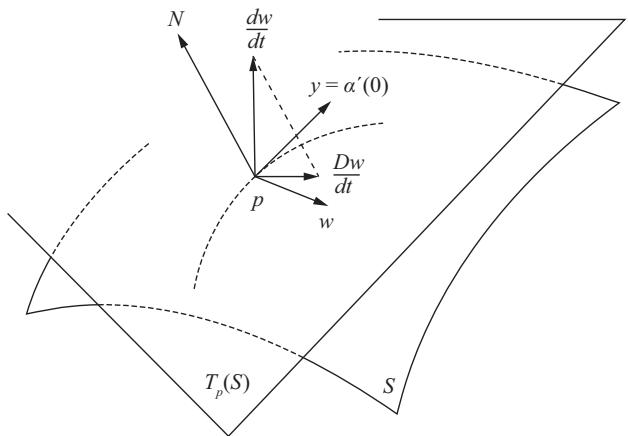
\includegraphics[width=\textwidth]{../../../PDFs/differential-geometry/transcript/Do Carmo - Differential Geometry of Curves and Surfaces/hybrid_ocr/images/a32e506ff2b166230093d24cd4de247d299f71e1ccc68eebbf2e35dc5fe64b2d.jpg}}
\end{minipage}
\end{figure}

通过参数化 $\mathbf{x}(u,v)$ 中的分量表达，共变导数只依赖于向量 $(u',v') = y$，而不依赖于曲线 $\alpha$ 的选择。表达式为：
\[
\frac{Dw}{dt} = \left(a' + \Gamma_{11}^1 a u' + \Gamma_{12}^1 a v' + \Gamma_{12}^1 b u' + \Gamma_{22}^1 b v'\right)\mathbf{x}_u
+ \left(b' + \Gamma_{11}^2 a u' + \Gamma_{12}^2 a v' + \Gamma_{12}^2 b u' + \Gamma_{22}^2 b v'\right)\mathbf{x}_v.
\label{eq:covariant-derivative}
\]

特别地，当 $S$ 是平面时（取 $E=G=1$，$F=0$），Christoffel 符号均为零，共变导数退化为平面上向量通常的导数。因此共变导数是平面向量微分在曲面情形下的自然推广。

\begin{Definition}[平行向量场]\label{def:parallel-field}
设 $\mathbf{w}$ 是沿曲线 $\alpha: I \to S$ 的可微向量场。若 $D\mathbf{w}/dt = 0$ 对所有 $t \in I$ 成立，则称 $\mathbf{w}$ 是\textbf{平行向量场}（parallel field along $\alpha$）。
\end{Definition}

\begin{Proposition}[平行场的保角性]\label{prop:parallel-preserves-angle}
沿曲线 $\alpha$ 的两个平行向量场 $\mathbf{w}$ 和 $\mathbf{v}$ 的内积 $\langle \mathbf{w}(t), \mathbf{v}(t) \rangle$ 为常数。特别地，$|\mathbf{w}(t)|$ 和 $|\mathbf{v}(t)|$ 为常数，$\mathbf{w}(t)$ 与 $\mathbf{v}(t)$ 之间的夹角也为常数。
\end{Proposition}

\begin{Proposition}[平行运输的存在唯一性]\label{prop:parallel-transport}
设 $\alpha: I \to S$ 是参数曲线，$w_0 \in T_{\alpha(t_0)}(S)$，$t_0 \in I$。则存在唯一的沿 $\alpha$ 的平行向量场 $\mathbf{w}(t)$，使 $\mathbf{w}(t_0) = w_0$。
\end{Proposition}

\begin{Definition}[平行运输]\label{def:parallel-transport}
设 $\alpha: I \to S$ 是参数曲线，$w_0 \in T_{\alpha(t_0)}(S)$。将 $w_0$ 沿 $\alpha$ 平行移动得到的向量场 $\mathbf{w}(t)$ 在 $t_1$ 处的值 $\mathbf{w}(t_1)$ 称为 $w_0$ 沿 $\alpha$ 在 $t_1$ 处的\textbf{平行运输}（parallel transport）。
\end{Definition}

平行运输的一个重要性质：若两曲面沿曲线 $\alpha$ 相切，则沿 $\alpha$ 的平行运输在两张曲面上相同。

\begin{Example}[球面上的平行运输]\label{ex:parallel-sphere}
单位球面 $S^2$ 上，纬线（平行圆）的切向量场若沿该纬线平移，则保持与纬线的夹角为常数（教材 Figure 4-11（见 \cref{fig:fig4-11}））。

具体地，设 $C$ 是余纬度为 $\varphi$ 的纬线，$w_0$ 是 $C$ 上某点处的单位切向量。沿 $C$ 平行运输一周后，向量相对于初始位置的转角为 $2\pi - \theta$（其中 $\theta$ 是中心角）。
\end{Example}

\begin{figure}[H]
\centering
\begin{minipage}{0.40\textwidth}
\centering
\subfloat[Figure 4-9. 曲线上的切向量场]{\label{fig:fig4-9}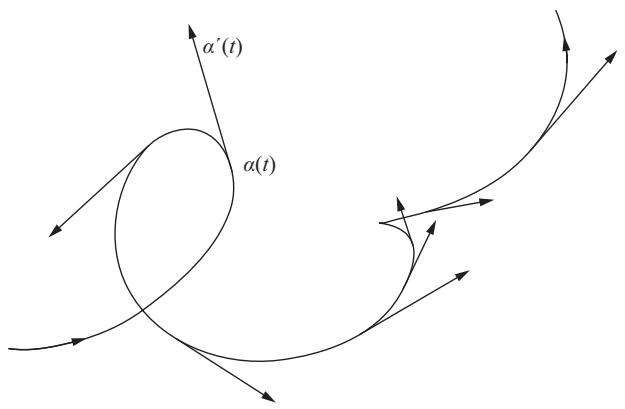
\includegraphics[width=\textwidth]{../../../PDFs/differential-geometry/transcript/Do Carmo - Differential Geometry of Curves and Surfaces/hybrid_ocr/images/58f013cc939f2f2be40e76a2123ccfee464e975b78b8ca5f24ae6d144405cdc9.jpg}}
\end{minipage}
\hfill
\begin{minipage}{0.55\textwidth}
\centering
\subfloat[Figure 4-10. 平面上的平行向量场]{\label{fig:fig4-10}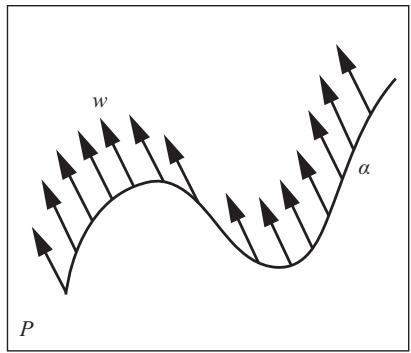
\includegraphics[width=\textwidth]{../../../PDFs/differential-geometry/transcript/Do Carmo - Differential Geometry of Curves and Surfaces/hybrid_ocr/images/3958b81e2e6b6026c3b6fa030678d6147aa26191c953a00e6118e0fa1cc14c82.jpg}}
\end{minipage}
\end{figure}

\begin{figure}[H]
\centering
\begin{minipage}{0.50\textwidth}
\centering
\subfloat[Figure 4-11. 球面上的平行场]{\label{fig:fig4-11}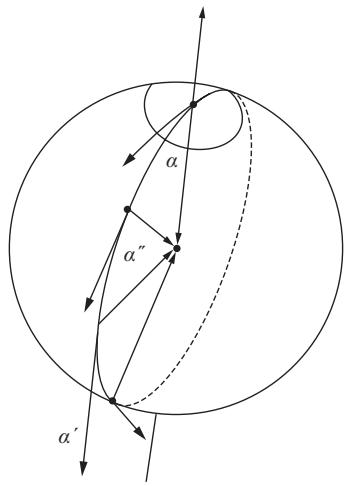
\includegraphics[width=\textwidth]{../../../PDFs/differential-geometry/transcript/Do Carmo - Differential Geometry of Curves and Surfaces/hybrid_ocr/images/7018de7d6cf0f188f91024eb14310c5a27e92fe83d6f94abce16bfd2e79c5b13.jpg}}
\end{minipage}
\hfill
\begin{minipage}{0.40\textwidth}
\centering
\subfloat[Figure 4-12. 纬线上平行运输的几何构造]{\label{fig:fig4-12}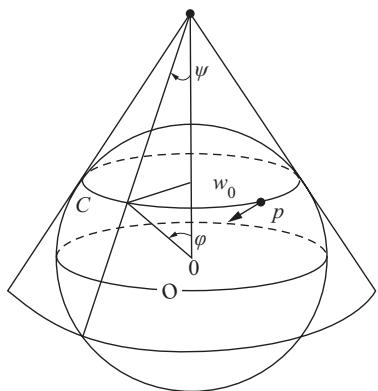
\includegraphics[width=\textwidth]{../../../PDFs/differential-geometry/transcript/Do Carmo - Differential Geometry of Curves and Surfaces/hybrid_ocr/images/52affde3eb1685ac8decd2bf0d621e9fae252c5ce15c16c7bb119ff2908cb49d.jpg}}
\end{minipage}
\end{figure}

\begin{figure}[H]
\centering
\begin{minipage}{0.45\textwidth}
\centering
\subfloat[Figure 4-13. 圆锥展开后的平行运输]{\label{fig:fig4-13}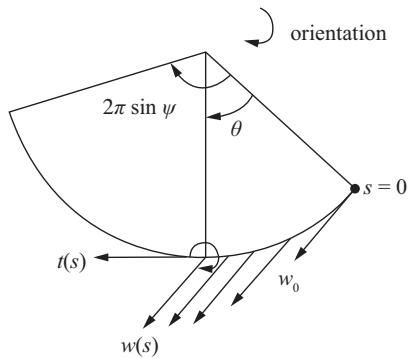
\includegraphics[width=\textwidth]{../../../PDFs/differential-geometry/transcript/Do Carmo - Differential Geometry of Curves and Surfaces/hybrid_ocr/images/7109502d0af63724e52fcde73cd54979936029dd6a250f7030f946fa9afa0e43.jpg}}
\end{minipage}
\end{figure}

\textbf{Geodesics.} 在平面上，切向量场平行的曲线正是直线。测地线是这一性质在曲面情形下的推广。

\begin{Definition}[测地线]\label{def:geodesic}
非平凡参数曲线 $\gamma: I \to S$ 称为在 $t \in I$ 处是\textbf{测地的}（geodesic at $t$），如果其切向量场 $\gamma'(t)$ 沿 $\gamma$ 在 $t$ 处平行，即
\[
\frac{D\gamma'(t)}{dt} = 0.
\]
若 $\gamma$ 对所有 $t \in I$ 均为测地的，则称其为\textbf{参数化测地线}（parametrized geodesic）。
\end{Definition}

由 \cref{prop:parallel-preserves-angle}，参数化测地线有 $| \gamma'(t) | = \mathrm{const} = c \neq 0$，因此可以取弧长 $s = ct$ 作为参数——即参数 $t$ 与弧长成正比。

从外蕴角度看，曲线 $C \subset S$（$k \neq 0$）是测地线，当且仅当其每点处的主法向量与曲面法向量平行——也就是说，曲线"尽可能直"。

\begin{Example}[球面的大圆是测地线]\label{ex:great-circles}
球面 $S^2$ 的大圆由过球心的平面与球面的交线得到。由于大圆是圆心在球心的圆，其主法向量指向圆心，从而与球面法向量一致。因此大圆是测地线。
\end{Example}

\begin{Example}[圆柱面上的测地线]\label{ex:cylinder-geodesics}
正圆柱面 $x^2+y^2=1$ 的测地线包括：母线（直线）和正交于轴的圆。具体地，圆柱面参数化 $\mathbf{x}(u,v) = (\cos u, \sin u, v)$ 下的测地线由方程组给出（教材 Figure 4-15（见 \cref{fig:fig4-15}））。除了直线和圆之外，螺旋线也是圆柱面的测地线——这是因为圆柱面去掉一条母线后等距于平面，而平面上两点之间的最短路径是直线，在圆柱面上对应的就是螺旋线。
\end{Example}

\begin{figure}[H]
\centering
\begin{minipage}{0.55\textwidth}
\centering
\subfloat[Figure 4-15. 圆柱面上的测地线：圆、螺旋线和母线]{\label{fig:fig4-15}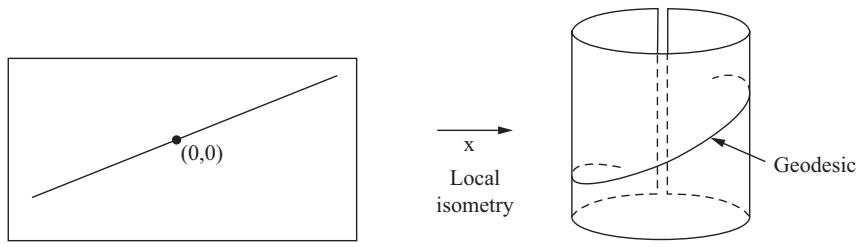
\includegraphics[width=\textwidth]{../../../PDFs/differential-geometry/transcript/Do Carmo - Differential Geometry of Curves and Surfaces/hybrid_ocr/images/8323f6615eba636857dda49d36c4c46af03766f13b7e6676e92675cdd47f30c2.jpg}}
\end{minipage}
\hfill
\begin{minipage}{0.40\textwidth}
\centering
\subfloat[Figure 4-16. 圆柱面上连接两点的无穷多条测地线]{\label{fig:fig4-16}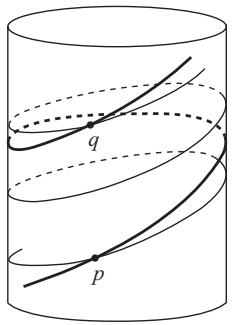
\includegraphics[width=\textwidth]{../../../PDFs/differential-geometry/transcript/Do Carmo - Differential Geometry of Curves and Surfaces/hybrid_ocr/images/7694cd790d84ea64dcbd613e30c8500ba9c0b49e6536e2fa626f8ed0e3efc2a1.jpg}}
\end{minipage}
\end{figure}

\begin{Proposition}[测地线的存在唯一性]\label{prop:geodesic-existence}
给定 $p \in S$ 和非零向量 $w \in T_p(S)$，存在 $\epsilon > 0$ 和唯一的参数化测地线 $\gamma: (-\epsilon, \epsilon) \to S$，使 $\gamma(0) = p$，$\gamma'(0) = w$。
\end{Proposition}

在正交参数化下，测地线的方程为：
\[
\begin{cases}
u'' + \Gamma_{11}^1 (u')^2 + 2\Gamma_{12}^1 u'v' + \Gamma_{22}^1 (v')^2 = 0,\\[2pt]
v'' + \Gamma_{11}^2 (u')^2 + 2\Gamma_{12}^2 u'v' + \Gamma_{22}^2 (v')^2 = 0.
\end{cases}
\label{eq:geodesic-equations}
\]

\textbf{Geodesic curvature.} 平面上曲线的曲率描述其偏离直线的程度。测地曲率是这一概念在曲面情形下的推广。

\begin{Definition}[测地曲率]\label{def:geodesic-curvature}
设 $C$ 是定向曲面 $S$ 上的有向正则曲线，$\alpha(s)$ 是以弧长为参数的邻域参数化。$C$ 在 $p$ 处的\textbf{测地曲率}（geodesic curvature）为代数值 $[D\alpha'(s)/ds] = k_g \alpha'(s)$。
\end{Definition}

测地线的特征是测地曲率为零（$k_g = 0$）。

Liouville 公式给出了正交参数化下测地曲率的表达式（教材 Figure 4-17 和 Figure 4-18（见 \cref{fig:fig4-17,fig:fig4-18}））：

\begin{Proposition}[Liouville 公式]\label{prop:liouville}
设 $\mathbf{x}(u,v)$ 是 $S$ 的正交参数化（$F=0$），$\alpha(s)$ 是有向正则曲线 $C$ 的弧长参数化，$\varphi(s)$ 是 $\mathbf{x}_u$ 与 $\alpha'(s)$ 之间的有向角。则
\[
k_g = (k_g)_1 \cos\varphi + (k_g)_2 \sin\varphi + \frac{d\varphi}{ds},
\label{eq:liouville}
\]
其中 $(k_g)_1$ 和 $(k_g)_2$ 分别是坐标曲线 $v=\mathrm{const}$ 和 $u=\mathrm{const}$ 的测地曲率。
\end{Proposition}

\begin{figure}[H]
\centering
\begin{minipage}{0.45\textwidth}
\centering
\subfloat[Figure 4-17. 曲率分解 $k^2 = k_g^2 + k_n^2$]{\label{fig:fig4-17}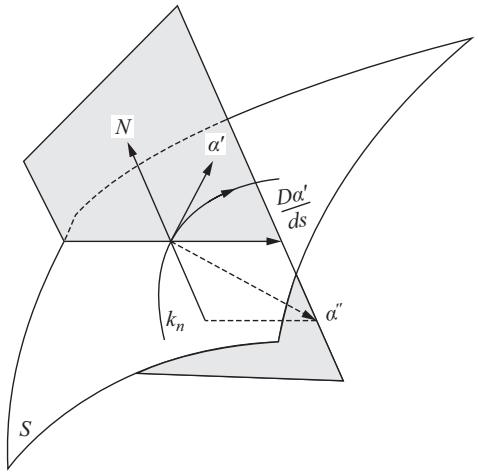
\includegraphics[width=\textwidth]{../../../PDFs/differential-geometry/transcript/Do Carmo - Differential Geometry of Curves and Surfaces/hybrid_ocr/images/f780bbd0905f1b1ff42460a1a48ea18d1b6f029b834695ae102ada481fe1bef4.jpg}}
\end{minipage}
\hfill
\begin{minipage}{0.45\textwidth}
\centering
\subfloat[Figure 4-18. 球面上纬线的测地曲率]{\label{fig:fig4-18}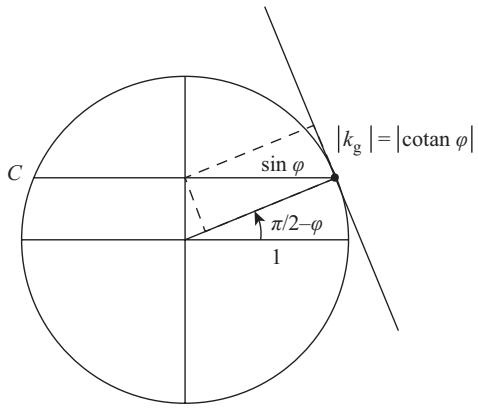
\includegraphics[width=\textwidth]{../../../PDFs/differential-geometry/transcript/Do Carmo - Differential Geometry of Curves and Surfaces/hybrid_ocr/images/6f369dfbf71de0885d0b4e3e5ea8c5179445092355b59bec0f01940e31eda3b1.jpg}}
\end{minipage}
\end{figure}

\begin{Remark}
测地曲率 $k_g$ 在以下情形下变号：改变曲线 $C$ 或曲面 $S$ 的定向。这与 $K$（由行列式定义）不同——$K$ 的符号与曲面定向无关。
\end{Remark}

\textbf{Clairaut's relation.} 对于旋转面上的测地线，有一个重要的几何关系。设旋转面 $S$ 由 $(f(v)\cos u,\; f(v)\sin u,\; g(v))$ 参数化，则由 \cref{eq:geodesic-equations} 的第一个方程可得
\[
f^2 u' = \mathrm{const} = c.
\label{eq:clairaut}
\]
设 $\theta$ 是测地线与纬线之间的夹角，则由第一基本形式可得
\[
\cos\theta = |fu'| = \frac{|c|}{f}.
\]
于是得到 Clairaut 关系：
\[
r\cos\theta = \mathrm{const} = |c|,
\]
其中 $r = f$ 是纬线半径。直观上：测地线到轴的距离与夹角余弦的乘积为常数（教材 Figure 4-19（见 \cref{fig:fig4-19}））。

\begin{figure}[H]
\centering
\begin{minipage}{0.55\textwidth}
\centering
\subfloat[Figure 4-19. Clairaut 关系：旋转面上测地线的几何约束]{\label{fig:fig4-19}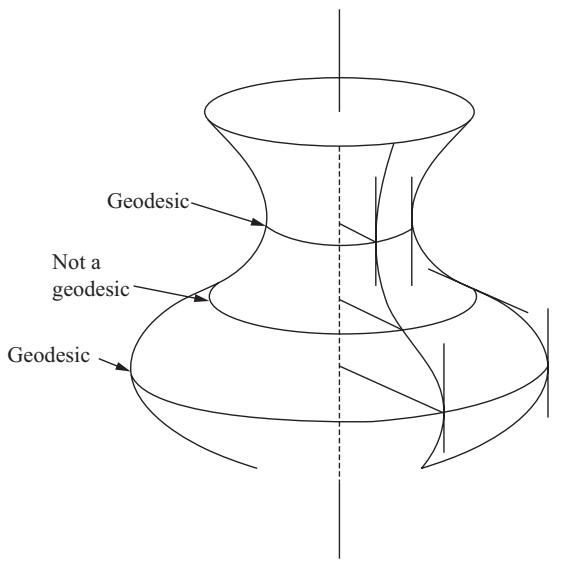
\includegraphics[width=\textwidth]{../../../PDFs/differential-geometry/transcript/Do Carmo - Differential Geometry of Curves and Surfaces/hybrid_ocr/images/bddaed62c0b6d28517e5ef538040464f3b623c4e2b10d084ae2ad82c9ad885ea.jpg}}
\end{minipage}
\end{figure}

Clairaut 关系的一个应用：抛物面 $z=x^2+y^2$ 上的非子午线测地线必与所有子午线相交，从而无限次自交（教材 Figure 4-20（见 \cref{fig:fig4-20}））。

\begin{figure}[H]
\centering
\begin{minipage}{0.60\textwidth}
\centering
\subfloat[Figure 4-20. 抛物面上测地线的自交现象]{\label{fig:fig4-20}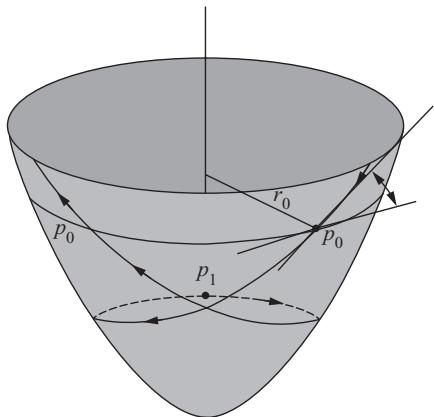
\includegraphics[width=\textwidth]{../../../PDFs/differential-geometry/transcript/Do Carmo - Differential Geometry of Curves and Surfaces/hybrid_ocr/images/9e8baf69971bdd20fbb97b03d9f9aa9ea0f562dcd33d692943ac15331035db86.jpg}}
\end{minipage}
\end{figure}

\begin{Remark}
与平面不同，曲面上两点之间可能有多条测地线（如圆柱面上同一点的不同螺旋线可以连接同一条纬线上的两点）。
\end{Remark}

\begin{Remark}
球面上每点每方向唯一确定一条大圆（测地线），但经过延伸后，较长的大圆弧不是连接两点的最短路径。
\end{Remark}

\begin{Remark}
教材 Figure 4-21（见 \cref{fig:fig4-21}）展示了球面上平行圆上平行运输一圈后的角度变化。
\end{Remark}

\begin{figure}[H]
\centering
\begin{minipage}{0.55\textwidth}
\centering
\subfloat[Figure 4-21. 球面上平行圆绕一圈后的角度变化]{\label{fig:fig4-21}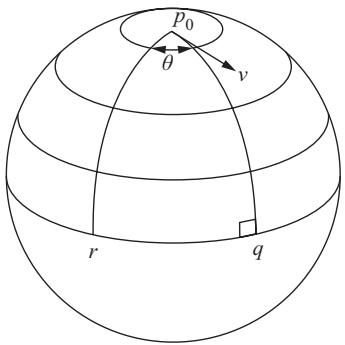
\includegraphics[width=\textwidth]{../../../PDFs/differential-geometry/transcript/Do Carmo - Differential Geometry of Curves and Surfaces/hybrid_ocr/images/810751630caccdbfbf1bea5762bf7dfb4a3ee7cf7d972163b1b3b3c4c86d80ab.jpg}}
\end{minipage}
\end{figure}

\begin{Remark}
教材 Figure 4-22（见 \cref{fig:fig4-22}）展示了单叶双曲面上一条特殊测地线趋近于赤道平行的有趣行为。
\end{Remark}

\begin{figure}[H]
\centering
\begin{minipage}{0.55\textwidth}
\centering
\subfloat[Figure 4-22. 单叶双曲面上测地线趋近于赤道]{\label{fig:fig4-22}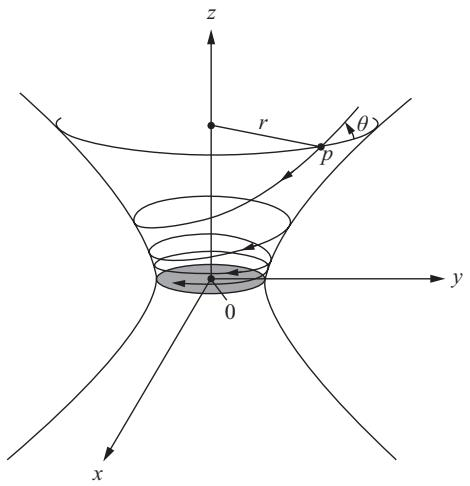
\includegraphics[width=\textwidth]{../../../PDFs/differential-geometry/transcript/Do Carmo - Differential Geometry of Curves and Surfaces/hybrid_ocr/images/254492eaf279a277aa50d663f514ffe71e1e0c24277de28a838e56cbe078ed0c.jpg}}
\end{minipage}
\end{figure}

\begin{Remark}
测地线的另一个有趣应用是关于直线面（ruled surface）的：若 $\alpha(s)$ 是挠率非零的曲线，$\mathbf{x}(s,v) = \alpha(s) + vb(s)$（其中 $b$ 是 $\alpha$ 的副法向量），则 $\mathbf{x}$ 是正则曲面，且 $\alpha$ 是该曲面上的测地线（教材习题 17）。
\end{Remark}

\begin{Remark}
教材 Figure 4-14（见 \cref{fig:fig4-14}）展示了沿一般曲线 $C$ 的平行运输的几何构造：通过沿 $C$ 的切平面族的包络面来实现。
\end{Remark}

\begin{figure}[H]
\centering
\begin{minipage}{0.60\textwidth}
\centering
\subfloat[Figure 4-14. 沿曲线 C 的平行运输构造]{\label{fig:fig4-14}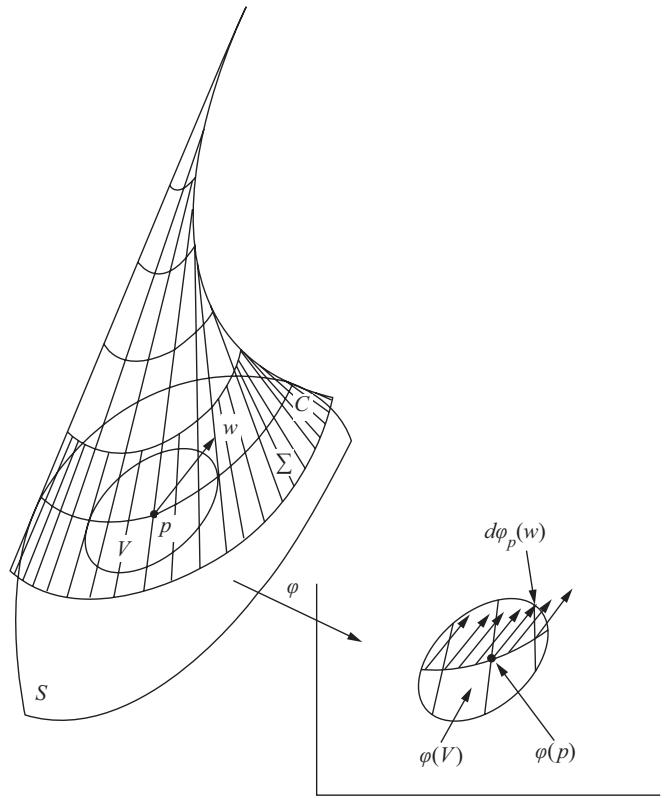
\includegraphics[width=\textwidth]{../../../PDFs/differential-geometry/transcript/Do Carmo - Differential Geometry of Curves and Surfaces/hybrid_ocr/images/cc21bcdb163bffebf68dbaae3c27f43c6b235a2f4b662a3aa56a256b1d3a950d.jpg}}
\end{minipage}
\end{figure}

\subsection*{4-4 节练习}

\begin{exercise}{4-4, 1 — do Carmo, Exercise 4-4, 1}
Let $y$ and $w$ be differentiable vector fields on an open set $U \subset S$. Let $p \in S$ and let $\alpha \colon I \to U$ be a curve such that $\alpha(0) = p$, $\alpha'(0) = y$. Denote by $P_{\alpha, t} \colon T_{\alpha(0)}(S) \to T_{\alpha(t)}(S)$ the parallel transport along $\alpha$ from $\alpha(0)$ to $\alpha(t)$, $t \in I$. Prove that

\[
(D_y w)(p) = \frac{d}{dt}\left(P_{\alpha, t}^{-1}(w(\alpha(t)))\right)\Bigg|_{t=0},
\]

where the second member is the velocity vector of the curve $P_{\alpha, t}^{-1}(w(\alpha(t)))$ in $T_p(S)$ at $t = 0$. (Thus, the notion of covariant derivative can be derived from the notion of parallel transport.)
\end{exercise}

\begin{solution}
\textbf{直观理解}: 共变导数本质上是将向量场沿曲线拉回初始切空间后的普通导数。平行运输将 $w(\alpha(t))$ 拉回到 $T_p(S)$ 中，其速度向量即为共变导数。

\textbf{解答}: 设 $P_{\alpha,t}: T_p(S) \to T_{\alpha(t)}(S)$ 为沿 $\alpha$ 从 $p$ 到 $\alpha(t)$ 的平行运输（它是一个等距）。则 $P_{\alpha,t}^{-1}$ 将切向量从 $T_{\alpha(t)}(S)$ 等距地拉回到 $T_p(S)$。考虑曲线 $t \mapsto P_{\alpha,t}^{-1}(w(\alpha(t)))$，它在 $t=0$ 时的速度向量即为右端表达式。

由平行运输的定义，$P_{\alpha,t}^{-1}(w(\alpha(t)))$ 在 $T_p(S)$ 中是 $w$ 沿 $\alpha$ 的共变导数的"平坦版本"。因此其速度向量等于 $D_yw(p)$，即共变导数。
\qed
\end{solution}

\begin{exercise}{4-4, 2 — do Carmo, Exercise 4-4, 2}
a. Show that the covariant derivative has the following properties. Let $v$, $w$, and $y$ be differentiable vector fields in $U \subset S$, $f \colon U \to \mathbb{R}$ be a differentiable function in $S$, $y(f)$ be the derivative of $f$ in the direction of $y$ (cf. Exercise 7, Sec. 3-4), and $\lambda$, $\mu$ be real numbers. Then

\begin{enumerate}
\item $D_y(\lambda v + \mu w) = \lambda D_y(v) + \mu D_\gamma(w)$;
\[
D_{\lambda y + \mu v}(w) = \lambda D_y(w) + \mu D_v(w).
\]
\item $D_y(fv) = y(f)v + fD_y(v)$; $D_{fy}(v) = fD_y(v)$.
\item $y(\langle v,w\rangle) = \langle D_yv,w\rangle +\langle v,D_yw\rangle$.
\item $D_{\mathbf{x}_v}\mathbf{x}_u = D_{\mathbf{x}_u}\mathbf{x}_v$, where $\mathbf{x}(u,v)$ is a parametrization of $S$.
\end{enumerate}

$^{^*}$\textbf{b}. Show that property 3 is equivalent to the fact that the parallel transport along a given piecewise regular parametrized curve $\alpha \colon I \to S$ joining two points $p, q \in S$ is an isometry between $T_p(S)$ and $T_q(S)$. Show that property 4 is equivalent to the symmetry of the lower indices of the Christoffel symbols.

$^{^*}$\textbf{c}. Let $\mathfrak{U}(U)$ be the space of (differentiable) vector fields in $U\subset S$ and let $D\colon \mathfrak{U}\times \mathfrak{U}\to \mathfrak{U}$ (where we denote $D(y,v) = D_y(v)$) be a map satisfying properties 1--4. Verify that $D_y(v)$ coincides with the covariant derivative of the text. (In general, a $D$ satisfying properties 1 and 2 is called a connection in $U$. The point of the exercise is to prove that on a surface with a given scalar product there exists a unique connection with the additional properties 3 and 4).
\end{exercise}

\begin{solution}
\textbf{直观理解}: 共变导数由四个基本性质刻画：线性性（性质1）、导子性（性质2）、保度规性（性质3）和对称性（性质4）。反过来，满足这些性质的映射只能是共变导数。

\textbf{解答}: a. 直接验证：性质1 由共变导数的线性定义；性质2 由导子的莱布尼茨规则；性质3 由平行运输保内积（性质3 $\Leftrightarrow$ 平行运输为等距）；性质4 由 Christoffel 符号的对称性 $\Gamma_{ij}^k = \Gamma_{ji}^k$。

b. 若性质3成立，即 $y(\langle v,w\rangle) = \langle D_yv,w\rangle + \langle v,D_yw\rangle$，对曲线 $\alpha$ 沿 $t$ 方向可得 $\frac{d}{dt}\langle v,w\rangle = \langle D_{\alpha'}v,w\rangle + \langle v,D_{\alpha'}w\rangle$。由习题1的解答，$D_{\alpha'}v$ 是 $v$ 的共变导数，其保内积性质等价于平行运输是等距。反之，若平行运输是等距，则沿曲线 $v$ 与 $w$ 的内积为常数，性质3 成立。性质4 等价于 $\Gamma_{ij}^k$ 的对称性 $\Gamma_{ij}^k = \Gamma_{ji}^k$。

c. 设 $D$ 满足 1--4，取正交参数化 $\mathbf{x}(u,v)$。令 $y = y_1\mathbf{x}_u+y_2\mathbf{x}_v$，$w = w_1\mathbf{x}_u+w_2\mathbf{x}_v$。由性质1、2、3 可推出 $D_yw$ 在每点由 $D_{\mathbf{x}_u}\mathbf{x}_u$、$D_{\mathbf{x}_u}\mathbf{x}_v$、$D_{\mathbf{x}_v}\mathbf{x}_v$ 决定，且这些量满足与 Christoffel 符号相同的方程（见教材第 4-3 节方程 (2)）。故 $A_{ij}^k = \Gamma_{ij}^k$，于是 $D_yv$ 恰好是"取普通导数并投影到切平面"的操作，与共变导数一致。唯一性由对称性（性质4）保证。
\qed
\end{solution}

\begin{exercise}{4-4, 3 — do Carmo, Exercise 4-4, 3}
Let $\alpha \colon I = [0, l] \to S$ be a simple, parametrized, regular curve. Consider a unit vector field $v(t)$ along $\alpha$, with $\langle \alpha'(t), v(t) \rangle = 0$ and a mapping $\mathbf{x} \colon \mathbb{R} \times I \to S$ given by

\[
\mathbf{x}(s, t) = \exp_{\alpha(t)}(s v(t)), \quad s \in \mathbb{R}, t \in I.
\]

a. Show that $\mathbf{x}$ is differentiable in a neighborhood of $I$ in $\mathbb{R}\times I$ and that $d\mathbf{x}$ is nonsingular in $(0,t), t\in I$.

b. Show that there exists $\epsilon > 0$ such that $\mathbf{x}$ is one-to-one in the rectangle $t \in I$, $|s| < \epsilon$.

c. Show that in the open set $t \in (0, l)$, $|s| < \epsilon$, $\mathbf{x}$ is a parametrization of $S$, the coordinate neighborhood of which contains $\alpha((0, l))$. The coordinates thus obtained are called geodesic coordinates (or Fermi's coordinates) of basis $\alpha$. Show that in such a system $F = 0$, $E = 1$. Moreover, if $\alpha$ is a geodesic parametrized by the arc length, $G(0, t) = 1$ and $G_s(0, t) = 0$.

d. Establish the following analogue of the Gauss lemma (Remark 1 after Prop. 3, Sec. 4-6). Let $\alpha \colon I \to S$ be a regular parametrized curve and let $\gamma_t(s), t \in I$, be a family of geodesics parametrized by arc length $s$ and given by $\gamma_t(0) = \alpha(t)$, $\{\gamma_t'(0), \alpha'(t)\}$ is a positive orthogonal basis. Then, for a fixed $\bar{s}$, sufficiently small, the curve $t \to \gamma_t(\bar{s})$, $t \in I$, intersects all $\gamma_t$ orthogonally (such curves are called geodesic parallels).
\end{exercise}

\begin{solution}
\textbf{直观理解}: 在 Fermi 坐标系下，测地线 $\gamma_t(s)$ 沿 $s$ 方向是平行的，而 Gauss 引理保证 $s$-曲线与 $t$-曲线正交。

\textbf{解答}: a. 由指数映射的可微性（标准 ODE 理论）和 $v(t)$ 的可微性，可得 $\mathbf{x}(s,t) = \exp_{\alpha(t)}(sv(t))$ 在 $I$ 的邻域内可微。且 $d\mathbf{x}_{(0,t)}(1,0) = v(t) \neq 0$，$d\mathbf{x}_{(0,t)}(0,1) = \alpha'(t) \neq 0$，故 $d\mathbf{x}$ 在 $(0,t)$ 处非奇异。

b. 由 (a) 的局部单射性和紧致性（Heine-Borel 定理），取 $\epsilon>0$ 充分小，使 $\mathbf{x}$ 在 $|s|<\epsilon$，$t\in I$ 上单射。

c. 由于 $d\mathbf{x}$ 非奇异，$\mathbf{x}$ 在上述开集上是 $S$ 的参数化。计算第一基本形式：$\langle\mathbf{x}_s,\mathbf{x}_t\rangle = F$，由性质4 的类比得 $F=0$；而 $|\mathbf{x}_s| = |\exp_{\alpha(t)*}v(t)| = |v(t)| = 1$，故 $E=1$。若 $\alpha$ 是测地线，则 $G(0,t)=1$，且 $G_s(0,t)=0$。

d. 由 (c)，$F=0$ 且 $E=1$，Gauss 引理成立：对固定的 $\bar{s}$，曲线 $t\mapsto\gamma_t(\bar{s})$ 与每条测地线 $\gamma_t$ 正交相交，称为测地平行线。
\qed
\end{solution}

\begin{exercise}{4-4, 4 — do Carmo, Exercise 4-4, 4}
The energy $E$ of a curve $\alpha \colon [a, b] \to S$ is defined by

\[
E(\alpha) = \int_a^b |\alpha'(t)|^2 \, dt.
\]

$^{^*}$\textbf{a}. Show that $(I(\alpha))^2 \leq (b - a)E(\alpha)$ and that equality holds if and only if $t$ is proportional to the arc length.

b. Conclude from part a that if $\gamma \colon [a,b]\to S$ is a minimal geodesic with $\gamma(a) = p$, $\gamma(b) = q$, then for any curve $\alpha \colon [a,b]\to S$, joining $p$ to $q$, we have $E(\gamma) \leq E(\alpha)$ and equality holds if and only if $\alpha$ is a minimal geodesic.
\end{exercise}

\begin{solution}
\textbf{直观理解}: 曲线的能量是弧长的平方在 Cauchy-Schwarz 不等式下的变分形式。最小化能量等价于最小化弧长。

\textbf{解答}: a. 设 $\alpha(t)$ 是以 $t$ 为参数的曲线。由 Cauchy-Schwarz 不等式：
\[
\left(\int_a^b |\alpha'(t)|\,dt\right)^2 \leq (b-a)\int_a^b |\alpha'(t)|^2\,dt,
\]
即 $L(\alpha)^2 \leq (b-a)E(\alpha)$。等号成立当且仅当 $|\alpha'(t)|$ 为常数，即 $t$ 与弧长成正比。

b. 若 $\gamma$ 是最短测地线（最小弧长连接 $p,q$），则对任意连接 $p,q$ 的曲线 $\alpha$，由 (a) 得 $L(\gamma)^2 \leq (b-a)E(\alpha)$。而 $L(\gamma) = |\gamma'(t)|(b-a)$，故 $E(\gamma) = |\gamma'|^2(b-a) = L(\gamma)^2/(b-a)$。于是 $E(\gamma) \leq E(\alpha)$，等号成立当且仅当 $|\alpha'(t)| = |\gamma'(t)| = \mathrm{const}$，即 $\alpha$ 也是最小测地线。
\qed
\end{solution}

\begin{exercise}{4-4, 5 — do Carmo, Exercise 4-4, 5}
Let $\gamma \colon [0,l] \to S$ be a simple geodesic, parametrized by arc length, and denote by $u$ and $v$ the Fermi coordinates in a neighborhood of $\gamma([0,l])$ which is given as $u = 0$ (cf. Exercise 3). Let $u = \gamma(v,t)$ be a family of curves depending on a parameter $t$, $-\epsilon < t < \epsilon$ such that $\gamma$ is differentiable and

\[
\gamma(0, t) = \gamma(0) = p, \quad \gamma(l, t) = \gamma(l) = q, \quad \gamma(v, 0) = \gamma(v) \equiv 0.
\]

Such a family is called a variation of $\gamma$ keeping the end points $p$ and $q$ fixed. Let $E(t)$ be the energy of the curve $\gamma(v, t)$ (cf. Exercise 4); that is,

\[
E(t) = \int_0^l \left(\frac{\partial \gamma}{\partial v}(v, t)\right)^2 \, dv.
\]

$^{^*}$\textbf{a}. Show that

\[
\begin{array}{l}
E'(0) = 0, \\[4pt]
\frac{1}{2} E''(0) = \int_0^l \left\{\left(\frac{d\eta}{dv}\right)^2 - K\eta^2\right\} dv,
\end{array}
\]

where $\eta(v) = \partial\gamma/\partial t|_{t=0}$, $K = K(v)$ is the Gaussian curvature along $\gamma$, and denotes the derivative with respect to $t$ (the above formulas are called the first and second variations, respectively, of the energy of $\gamma$; a more complete treatment of these formulas, including the case where $\gamma$ is not simple, will be given in Sec. 5-4).

b. Conclude from part a that if $K \leq 0$, then any simple geodesic $\gamma \colon [0, l] \to S$ is minimal relatively to the curves sufficiently close to $\gamma$ and joining $\gamma(0)$ to $\gamma(l)$.
\end{exercise}

\begin{solution}
\textbf{直观理解}: 第一变分给出 $E'(0)=0$（临界点条件），第二变分给出 $E''(0) = \int_0^l(|\eta'|^2 - K\eta^2)\,dv$。当 $K\leq 0$ 时，$-K\geq 0$，故 $E''(0)\geq 0$，说明 $E$ 在 $\gamma$ 处达到局部最小值。

\textbf{解答}: a. 设 $E(t) = \int_0^l |\partial\gamma/\partial v|^2\,dv$。对 $t$ 求导：$E'(t) = \int_0^l 2\langle\partial\gamma/\partial v,\partial^2\gamma/\partial v\partial t\rangle\,dv$。当 $t=0$ 时，$\partial\gamma/\partial v|_{t=0} = 0$，故 $E'(0)=0$。

第二变分：利用 $G_{uu} = -2K\sqrt{G}$ 和 $\sqrt{G}=1$（在 $t=0$ 处），得
\[
\frac{1}{2}E''(0) = \int_0^l\left(|\eta'(v)|^2 - K(v)\eta(v)^2\right)\,dv,
\]
其中 $\eta(v) = \partial\gamma/\partial t|_{t=0}$。

b. 若 $K\leq 0$，则 $K\eta^2\leq 0$，$|\eta'|^2 - K\eta^2 \geq |\eta'|^2 \geq 0$，于是 $E''(0) \geq 0$。因此能量 $E$ 在 $t=0$ 处达到局部最小值，$\gamma$ 相对于充分接近它的曲线是局部最小（最小测地线）。
\qed
\end{solution}

\begin{exercise}{4-4, 6* — do Carmo, Exercise 4-4, 6}
Let $S$ be the cone $z = k\sqrt{x^2 + y^2}$, $k > 0$, $(x, y) \neq (0, 0)$, and let $V \subset \mathbb{R}^2$ be the open set of $\mathbb{R}^2$ given in polar coordinates by $0 < \rho < \infty$, $0 < \theta < 2\pi n \sin \beta$, where $\cot \alpha = k$ and $n$ is the largest integer such that $2\pi n \sin \beta < 2\pi$ (cf. Example 3, Sec. 4-2). Let $\varphi: V \to S$ be the map

\[
\varphi(\rho, \theta) = \left(\rho \sin \beta \cos \left(\frac{\theta}{\sin \beta}\right), \rho \sin \beta \sin \left(\frac{\theta}{\sin \beta}\right), \rho \cos \beta\right).
\]

a. Prove that $\varphi$ is a local isometry.

b. Let $q \in S$. Assume that $\beta < \pi / 6$ and let $k$ be the largest integer such that $2\pi k \sin \beta < \pi$. Prove that there exist at least $k$ geodesics that leaving from $q$ return to $q$. Show that these geodesics are broken at $q$ and that, therefore, none of them is a closed geodesic (Fig. 4-49).

$^{^*}$\textbf{c}. Under the conditions of part b, prove that there are exactly $k$ such geodesics.
\end{exercise}

\begin{solution}
\textbf{直观理解}: 锥面通过展开映射与平面局部等距。在平面上，从一点出发并返回的直线（测地线）对应于扇形的两条边界；圆锥面上从 $q$ 出发并返回的测地线对应于展开平面中从原点出发的直线段。

\textbf{解答}: a. 设 $\cot\alpha=k$，$\sin\beta = 1/\sqrt{1+k^2}$。直接计算 $\varphi$ 的微分可得第一基本形式为 $E=1$，$F=0$，$G=1$（平面的标准形式），故 $\varphi$ 是局部等距。

b. 取 $\epsilon>0$ 充分小，考虑点 $(\rho,\epsilon)=r_0$，$(\rho,\epsilon+2\pi\sin\beta)=r_1$，$\ldots$，$(\rho,\epsilon+2\pi k\sin\beta)=r_k$。线段 $\overline{r_0r_1},\ldots,\overline{r_0r_k}$ 属于 $V$。由于 $\varphi$ 是局部等距，这些线段的像是从 $q=\varphi(r_0)$ 出发的测地线，且 $\varphi(r_j)=q$（$j=1,\ldots,k$）。这些测地线在 $q$ 处断开（因展开映射在圆周一圈后不重合），故不是闭测地线。

c. 需证每条从 $q$ 出发并返回的测地线恰好是某个线段 $\overline{r_0r_j}$（$j=1,\ldots,k$）的像。设 $\gamma:[0,l]\to S$ 是从 $q$ 到 $q$ 的测地线。取 $U\subset V$ 为 $r_0$ 的邻域，使 $\varphi|_U$ 是等距，则 $\tilde{\gamma} = \varphi^{-1}\circ\gamma$ 是从 $r_0$ 出发的直线段。由于 $\gamma(l)=q$，$\tilde{\gamma}$ 必经过某点 $r_j$（$j=1,\ldots,k$），故 $\gamma$ 是 $\overline{r_0r_j}$ 的像。恰有 $k$ 条。
\qed
\end{solution}

\begin{exercise}{4-4, 7 — do Carmo, Exercise 4-4, 7}
Let $\alpha: I \to \mathbb{R}^3$ be a parametrized regular curve. For each $t \in I$, let $P(t) \subset \mathbb{R}^3$ be a plane through $\alpha(t)$ which contains $\alpha'(t)$. When the unit normal vector $N(t)$ of $P(t)$ is a differentiable function of $t$ and $N'(t) \neq 0$, $t \in I$, we say that the map $t \to \{\alpha(t), N(t)\}$ is a differentiable family of tangent planes. Given such a family, we determine a parametrized surface (cf. Def. 2, Sec. 2-3) by

\[
\mathbf{x}(t, v) = \alpha(t) + v \frac{N(t) \wedge N'(t)}{|N'(t)|}.
\]

The parametrized surface $\mathbf{x}$ is called the envelope of the family $\{\alpha(t), N(t)\}$ (cf. Example 4, Sec. 3-5).

a. Let $S$ be an oriented surface and let $\gamma \colon I \to S$ be a geodesic parametrized by arc length with $k(s) \neq 0$ and $\tau(s) \neq 0$, $s \in I$. Let $N(s)$ be the unit normal vector of $S$ along $\gamma$. Prove that the envelope of the family of tangent planes $\{\gamma(s), N(s)\}$ is regular in a neighborhood of $\gamma$, has Gaussian curvature $K \equiv 0$, and is tangent to $S$ along $\gamma$. (Thus, we have obtained a surface locally isometric to the plane which contains $\gamma$ as a geodesic.)

b. Let $\alpha \colon I \to \mathbb{R}^3$ be a curve parametrized by arc length with $k(s) \neq 0$ and $\tau(s) \neq 0$, $s \in I$, and let $\{\alpha(s), n(s)\}$ be the family of its rectifying planes. Prove that the envelope of this family is regular in a neighborhood of $\alpha$, has Gaussian curvature $K = 0$, and contains $\alpha$ as a geodesic. (Thus, every curve is a geodesic in the envelope of its rectifying planes; since this envelope is locally isometric to the plane, this justifies the name rectifying plane.)
\end{exercise}

\begin{solution}
\textbf{直观理解}: 切平面的包络面恰好沿曲线展开为平面——曲线的副法向量给出展开方向，使曲线成为该平面曲面上的一条测地线。

\textbf{解答}: a. 设 $\gamma(s)$ 是 $S$ 上以弧长为参数的测地线，$k(s)\neq 0$，$\tau(s)\neq 0$。设 $N(s)$ 是 $S$ 沿 $\gamma$ 的单位法向量，则切平面族 $\{\gamma(s),N(s)\}$ 的包络面为
\[
\mathbf{x}(s,v) = \gamma(s) + v\frac{N(s)\wedge N'(s)}{|N'(s)|}.
\]
直接计算 $\mathbf{x}_s$ 和 $\mathbf{x}_v$ 的内积得 $F=0$，且 $E=1$（因为 $|N\wedge N'|/|N'|=|N'|=|N\times N'|=|dN|$，与曲线的法向导数有关）。由于沿 $\gamma$ 有 $D_{\gamma'}N = 0$（$N$ 与测地线法向量的关系），包络面的高斯曲率 $K\equiv 0$（可展曲面）。包络面在 $\gamma$ 处与 $S$ 相切。

b. 对任意曲线 $\alpha(s)$（$k\neq 0$，$\tau\neq 0$），取其密切平面族 $\{\alpha(s),n(s)\}$（即 $n(s)$ 为主法向量）。包络面 $\mathbf{x}(s,v) = \alpha(s)+v\frac{n(s)\wedge n'(s)}{|n'(s)|}$。由于 $n(s)\wedge n'(s)$ 指向 $\alpha$ 的切线方向（由 frenet 公式），包络面在 $v=0$ 处恰好为 $\alpha$，且 $\alpha$ 的切向量场沿包络面是平行的（$D_{\alpha'}\alpha'=0$），故 $\alpha$ 是该包络面上的测地线。其高斯曲率 $K=0$，因为包络面可展（沿直线方向展开）。
\qed
\end{solution}

\begin{exercise}{4-4, 8* — do Carmo, Exercise 4-4, 8}
(Free Mobility of Small Geodesic Triangles.) Let $S$ be a surface of constant Gaussian curvature. Choose points $p_1, p_1' \in S$ and let $V, V'$ be convex neighborhoods of $p_1, p_1'$, respectively. Choose geodesic triangles $p_1, p_2, p_3$ in $V$ (geodesic means that the sides $\widehat{p_1p_2}, \widehat{p_2p_3}, \widehat{p_3p_1}$ are geodesic arcs) in $v$ and $p_1', p_2', p_3'$ in $V'$ in such a way that

\[
\begin{array}{l}
l(p_1, p_2) = l\left(p_1', p_2'\right), \\
l(p_2, p_3) = l\left(p_2', p_3'\right), \\
l(p_3, p_1) = l\left(p_3', p_1'\right)
\end{array}
\]

(here $l$ denotes the length of a geodesic arc). Show that there exists an isometry $\theta \colon V \to V'$ which maps the first triangle onto the second. (This is the local version, for surfaces of constant curvature, of the theorem of high school geometry that any two triangles in the plane with equal corresponding sides are congruent.)
\end{exercise}

\begin{solution}
\textbf{直观理解}: 在常高斯曲率曲面上，测地三角形的边长完全决定了三角形的形状（直到等距）。这推广了平面几何中"SSS"全等判定。

\textbf{解答}: 设 $S$ 具有常数高斯曲率 $K$。在常曲率曲面上，局部存在等温坐标，使 $E=G=\lambda^2$，$F=0$，且 $K = -\frac{1}{\lambda^2}\Delta\log\lambda = \mathrm{const}$。由已知条件，两三角形的对应边长相等，故在平面模型（曲率 $K$ 对应的常曲率平面）中有相同边长的三角形全等。由于 $V$ 和 $V'$ 均为常曲率 $K$ 的局部等距模型中的邻域，利用等距的唯一性（局部保距映射由边界条件唯一确定），存在唯一的等距 $\theta: V\to V'$ 将第一个三角形映射到第二个。

更精确地说：在常曲率 $K$ 的曲面上，测地三角形由其边长唯一决定（直到等距运动），这可以通过建立局部坐标系（使得基点 $p_1$ 处 $u=v=0$，第一边沿 $u$ 轴）并利用测地线方程的唯一性证明。因此边长相等意味着存在等距变换 $\theta$ 将两三角形对应起来。
\qed
\end{solution}

% ==================== Section 4-5: The Gauss-Bonnet Theorem and Its Applications ====================
\section{The Gauss-Bonnet Theorem and Its Applications}\label{sec:gauss-bonnet}

\textbf{The crown jewel of surface theory.} Gauss-Bonnet 定理是曲面微分几何中最深刻的定理。它建立了曲面的拓扑（通过 Euler 示性数）与曲率（通过积分）之间的基本联系。

我们先从局部版本开始。

\textbf{Geodesic triangles.} 首先考虑测地三角形（三角形三边均为测地线弧）。Gauss 的原始版本为：

\[
\sum_{i=1}^3 \varphi_i - \pi = \iint_T K\, d\sigma,
\label{eq:gauss-original}
\]
其中 $\varphi_i$ 是内角，$T$ 是三角形区域（教材 Figure 4-23（见 \cref{fig:fig4-23}））。

直观含义：
\begin{itemize}
\item $K \equiv 0$（平面）时，$\sum\varphi_i = \pi$——Thales 定理的推广。
\item $K \equiv 1$（单位球面）时，$\sum\varphi_i - \pi = \mathrm{area}(T) > 0$——球面上测地三角形内角和大于 $\pi$。
\item $K \equiv -1$（伪球面）时，$\sum\varphi_i < \pi$——双曲几何的开端（教材 Figure 4-24（见 \cref{fig:fig4-24}））。
\end{itemize}

\begin{figure}[H]
\centering
\begin{minipage}{0.40\textwidth}
\centering
\subfloat[Figure 4-23. 球面上的测地三角形]{\label{fig:fig4-23}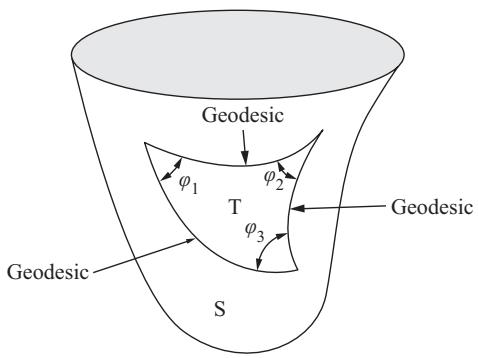
\includegraphics[width=\textwidth]{../../../PDFs/differential-geometry/transcript/Do Carmo - Differential Geometry of Curves and Surfaces/hybrid_ocr/images/7f17a66799fbba53c988fe3de929e1c81e7e2d8ac32746b6a23a4f32b55cf802.jpg}}
\end{minipage}
\hfill
\begin{minipage}{0.50\textwidth}
\centering
\subfloat[Figure 4-24. 不同曲率曲面上的测地三角形内角和]{\label{fig:fig4-24a}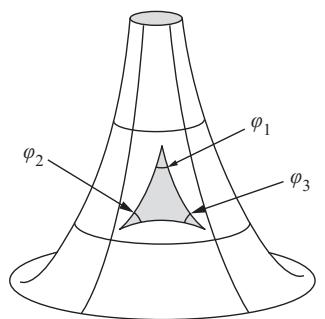
\includegraphics[width=\textwidth]{../../../PDFs/differential-geometry/transcript/Do Carmo - Differential Geometry of Curves and Surfaces/hybrid_ocr/images/e9e8f241c48b4fe66fd41816cf53fa20108e0888ae882ff02d856598209a91a6.jpg}}
\end{minipage}
\end{figure}

\begin{figure}[H]
\centering
\begin{minipage}{0.40\textwidth}
\centering
\subfloat[$K\equiv -1,\; \sum\varphi_i < \pi$]{\label{fig:fig4-24b}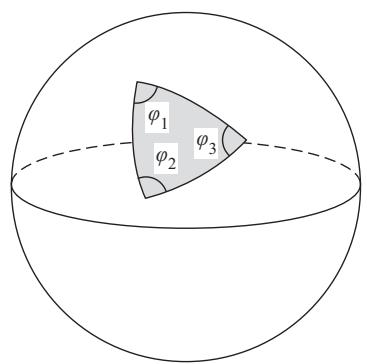
\includegraphics[width=\textwidth]{../../../PDFs/differential-geometry/transcript/Do Carmo - Differential Geometry of Curves and Surfaces/hybrid_ocr/images/6ff282221ad4338e008ce434e211a533767de832b7c2c8f811ad3e3b04447d26.jpg}}
\end{minipage}
\end{figure}

\textbf{Local Gauss-Bonnet theorem.} 现在给出局部 Gauss-Bonnet 定理的完整陈述。首先需要一些定义。

\begin{Definition}[简单闭分段正则曲线]\label{def:simple-closed-piecewise}
映射 $\alpha: [0,l] \to S$ 称为\textbf{简单闭分段正则参数曲线}，如果：
\begin{enumerate}
\item $\alpha(0) = \alpha(l)$；
\item $t_1 \neq t_2$（$t_1,t_2 \in [0,l)$）时 $\alpha(t_1) \neq \alpha(t_2)$；
\item 存在分划 $0 = t_0 < t_1 < \dots < t_k < t_{k+1} = l$，使 $\alpha$ 在每个 $(t_i, t_{i+1})$ 上是正则曲线。
\end{enumerate}
\end{Definition}

点 $\alpha(t_i)$ 称为 $\alpha$ 的\textbf{顶点}（vertices），$\alpha([t_i,t_{i+1}])$ 称为 $\alpha$ 的\textbf{正则弧}（regular arcs）。

\begin{Definition}[外角]\label{def:external-angle}
设 $S$ 定向，$|\theta_i|$（$0 \leq |\theta_i| < \pi$）是从 $\alpha'(t_i-0)$ 到 $\alpha'(t_i+0)$ 的最小转角的有向值。若非尖点（$|\theta_i| \neq \pi$），则 $\theta_i$ 的符号由定向决定。若 $|\theta_i| = \pi$（尖点），则 $\theta_i = \pm\pi$，由曲线在尖点处的两侧方向决定（教材 Figure 4-25 和 Figure 4-26（见 \cref{fig:fig4-25,fig:fig4-26}））。
\end{Definition}

\begin{figure}[H]
\centering
\begin{minipage}{0.45\textwidth}
\centering
\subfloat[Figure 4-25. 外角的定义]{\label{fig:fig4-25}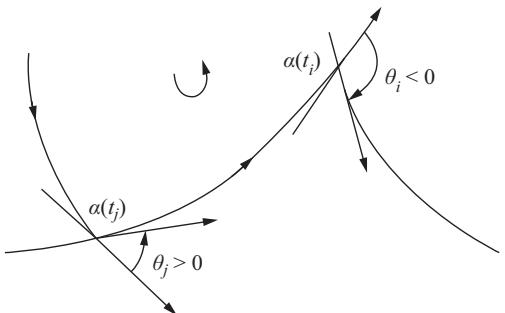
\includegraphics[width=\textwidth]{../../../PDFs/differential-geometry/transcript/Do Carmo - Differential Geometry of Curves and Surfaces/hybrid_ocr/images/692e99bb5f3b4a1db58e8a343b95ecc8bf19d1e5a2901bc6a7b8e1a069f285d3.jpg}}
\end{minipage}
\hfill
\begin{minipage}{0.45\textwidth}
\centering
\subfloat[Figure 4-26. 尖点处外角的符号]{\label{fig:fig4-26}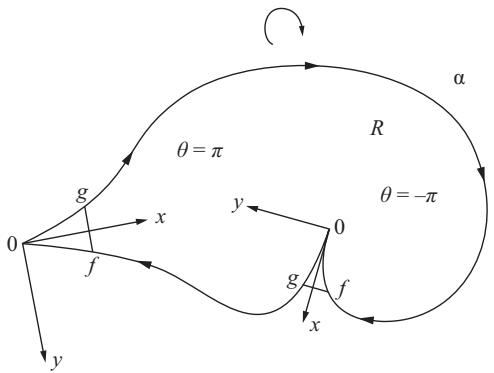
\includegraphics[width=\textwidth]{../../../PDFs/differential-geometry/transcript/Do Carmo - Differential Geometry of Curves and Surfaces/hybrid_ocr/images/eebe4d082414c2dc89923824b12008640d791e9d08af11a826d687e8e1363825.jpg}}
\end{minipage}
\end{figure}

\begin{Theorem}[Turning Tangents 定理]\labelthm:turning-tangents}
设 $\alpha$ 是如上定义的分段正则闭曲线，$\varphi_i$ 是从固定方向到第 $i$ 段弧切向量的转角函数。则
\[
\sum_{i=0}^k \left(\varphi_i(t_{i+1}) - \varphi_i(t_i)\right) + \sum_{i=0}^k \theta_i = \pm 2\pi,
\]
其中符号取决于 $\alpha$ 的定向。
\end{Theorem}

\begin{Definition}[正向边界]\label{def:positive-orientation}
设 $R \subset S$ 是简单区域（与圆盘同胚），$\partial R = \alpha(I)$ 是其边界。若沿 $\alpha$ 正向行走并使头指向 $N$ 时，区域 $R$ 总在左侧，则称 $\alpha$ 是\textbf{正向定向}的（教材 Figure 4-27（见 \cref{fig:fig4-27}））。
\end{Definition}

\begin{figure}[H]
\centering
\begin{minipage}{0.55\textwidth}
\centering
\subfloat[Figure 4-27. 正向定向的边界曲线]{\label{fig:fig4-27}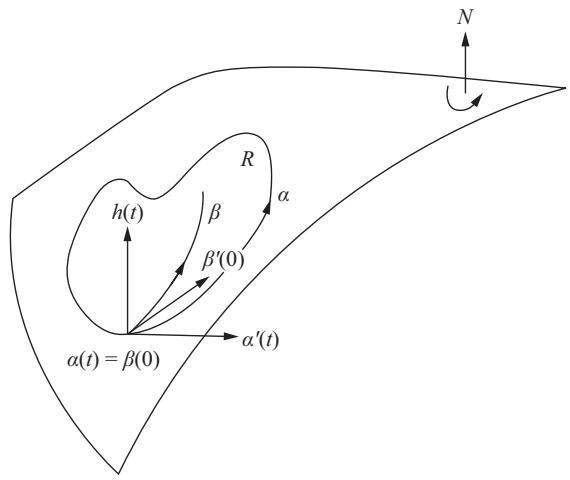
\includegraphics[width=\textwidth]{../../../PDFs/differential-geometry/transcript/Do Carmo - Differential Geometry of Curves and Surfaces/hybrid_ocr/images/2888e12eef0e0124556067081fa4cf88b516d79283e4052cde21bcf2d374e4e5.jpg}}
\end{minipage}
\end{figure}

现在可以陈述局部 Gauss-Bonnet 定理。

\begin{Theorem}[Gauss-Bonnet 定理（局部版本）]\labelthm:gauss-bonnet-local}
设 $\mathbf{x}: U \to S$ 是等温参数化（$F=0$，$E=G=\lambda^2$），$R \subset \mathbf{x}(U)$ 是有界简单区域，$\alpha: I \to S$ 是 $\partial R = \alpha(I)$ 的正向弧长参数化，$\alpha(s_0),\dots,\alpha(s_k)$ 和 $\theta_0,\dots,\theta_k$ 分别是其顶点和外角。则
\[
\sum_{i=0}^k \int_{s_i}^{s_{i+1}} k_g(s)\, ds + \iint_R K\, d\sigma + \sum_{i=0}^k \theta_i = 2\pi,
\label{eq:gauss-bonnet-local}
\]
其中 $k_g$ 是正则弧的测地曲率，$K$ 是 $S$ 的 Gaussian 曲率。
\end{Theorem}

\begin{Remark}
当 $R$ 是测地三角形时，$k_g = 0$ 在每条边上，且外角 $\theta_i = \pi - \varphi_i$（$\varphi_i$ 为内角），于是 \cref{eq:gauss-bonnet-local} 化为 $\sum \varphi_i - \pi = \iint_T K\, d\sigma$——Gauss 的原始版本。
\end{Remark}

\textbf{Global Gauss-Bonnet theorem.} 为了得到整体版本，我们需要拓扑概念。

设 $S$ 是紧致定向曲面，$R_1, \dots, R_n$ 是将 $S$ 分割为若干简单区域的测地多边形。令 $\chi(S) = \sum_{i=1}^n v_i - e + f$ 为 $S$ 的 Euler 示性数（其中 $v_i$ 是顶点数，$e$ 是边数，$f=n$ 是面数）。

\begin{Theorem}[Gauss-Bonnet 定理（整体版本）]\labelthm:gauss-bonnet-global}
设 $S$ 是紧致定向曲面。则
\[
\iint_S K\, d\sigma = 2\pi\chi(S).
\]
\end{Theorem}

\begin{Corollary}[紧致曲面总曲率的拓扑约束]\label{cor:total-curvature}
\[
\iint_S K\, d\sigma = 2\pi\chi(S) = 2\pi(2-2g - b),
\]
其中 $g$ 是亏格（genus），$b$ 是边界分支数。特别地：
\begin{itemize}
\item 若 $K > 0$ 在某开集上，则该区域对 Euler 示性数贡献正数；
\item 若 $K \leq 0$ 在整个 $S$ 上，则 $\chi(S) \leq 0$，从而 $g \geq 1$ 或 $b \geq 2$。
\end{itemize}
\end{Corollary}

Gauss-Bonnet 定理的一个直接推论是著名的 Poincaré-Hopf 定理的特殊情形：

\begin{Corollary}[曲率积分与 Euler 示性数]\label{cor:curvature-euler}
紧致曲面的总曲率仅由其拓扑决定，与具体形状无关。例如，环面（$g=1$，$b=0$）的 $\chi = 0$，无论其如何嵌入 $\mathbb{R}^3$，总满足 $\iint K\, d\sigma = 0$。
\end{Corollary}

\begin{Remark}
Gauss-Bonnet 定理是微分几何与拓扑学之间的第一座桥梁。它的深远影响在于：局部定义的曲率（通过微分）通过积分与整体拓扑（Euler 示性数）建立了等价关系。这一思想在现代几何中无处不在——Gauss-Bonnet 定理是 Atiyah-Singer 指标定理的特殊情形。
\end{Remark}

\subsection*{4-5 节练习}

\begin{exercise}{4-5, 1 — do Carmo, Exercise 4-5, 1}
设 $S \subset \mathbb{R}^3$ 是正则紧致连通定向曲面，且不同胚于球面。证明：$S$ 上必有这样一些点，其 Gaussian 曲率分别为正、负和零。
\end{exercise}

\begin{solution}
\textbf{直观理解}: 紧致曲面 $S$ 若不同胚于球面，则其 Euler 示性数 $\chi(S) \leq 0$。由 Gauss-Bonnet 定理，$\iint_S K\, d\sigma = 2\pi\chi(S) \leq 0$。若 $K$ 始终为正，则 $\chi(S) > 0$（球面情形）；若 $K$ 始终非正，则 $\iint_S K\, d\sigma \leq 0$，但不能恒等于零（否则 $S$ 为平坦环面等，拓扑类型不同胚于 $S$）。因此 $K$ 必在某处取正值、某处取负值，且由连续性在某些处为零。

\textbf{解答}: 设 $S$ 紧致连通定向，且 $\chi(S) \neq 2$（即不同胚于球面）。由 Gauss-Bonnet 定理，$\iint_S K\, d\sigma = 2\pi\chi(S)$。

若 $K > 0$ 在整个 $S$ 上成立，则 $\iint_S K\, d\sigma > 0$，从而 $\chi(S) > 0$。但由曲面分类定理，紧致连通曲面若 $\chi > 0$ 必同胚于球面，矛盾。

若 $K < 0$ 在整个 $S$ 上成立，则 $\iint_S K\, d\sigma < 0$，$\chi(S) < 0$，即 $S$ 至少有 $2$ 个"洞"（亏格 $g \geq 2$），此时 $S$ 不同胚于球面——但题目条件仅要求存在正、负、零三种曲率点，不需要讨论。

若 $K \leq 0$ 在整个 $S$ 上成立，则 $\iint_S K\, d\sigma \leq 0$，即 $\chi(S) \leq 0$。此时 $S$ 必同胚于环面（$\chi=0$）或亏格更高的曲面（$\chi<0$）。由于 $S$ 不是平坦曲面（平坦曲面的高斯曲率恒为零，则 $\chi(S)=0$，只能是环面），且 $S$ 紧致，故 $K$ 必在某处为正（考虑 $S$ 上的极大值点，由第二基本形式可得）。同理，由对称性 $K$ 也在某处为负。若 $K$ 恒负，则由 Hadamard 定理（$K<0$ 的紧致曲面必同胚于圆环面或更高亏格面），此时 $S$ 的亏格 $g \geq 1$，而 $\chi(S)=2-2g \leq 0$，但 $\iint_S K\, d\sigma = 2\pi\chi(S) < 0$ 仍可成立——此时需要 $K$ 在某处为零点（若 $K<0$ 恒负，则 $\iint_S K\, d\sigma$ 与 $\chi(S)$ 同号；若 $\chi(S)=0$（环面），则 $\iint_S K\, d\sigma=0$，由 $K<0$ 不可积得零，矛盾）。

综上，由曲面分类和连续性，$K$ 在 $S$ 上必既有正值点，也有负值点，同时必有点满足 $K=0$。
\qed
\end{solution}

\begin{exercise}{4-5, 2 — do Carmo, Exercise 4-5, 2}
设 $T$ 是旋转环面。描述 $T$ 的 Gauss 映射的像，并在不使用 Gauss-Bonnet 定理的情况下证明
\[
\iint_T K\, d\sigma = 0.
\]
计算 $T$ 的 Euler-Poincaré 示性数，并用 Gauss-Bonnet 定理验证上述结果。
\end{exercise}

\begin{solution}
\textbf{直观理解}: 旋转环面的 Gauss 映射将曲面上每点的法向量映射到单位球面上。由于环面同时有"外侧"（正高斯曲率区域）和"内侧"（负高斯曲率区域），其 Gauss 映射的像覆盖整个 $S^2$ 两次（正区一次，负区一次），两部分面积相等符号相反，故积分抵消为零。

\textbf{解答}: 设旋转环面由 $( (R + r\cos\varphi)\cos\theta,\; (R+r\cos\varphi)\sin\theta,\; r\sin\varphi )$ 给出，其中 $R>r>0$，$\theta,\varphi \in [0,2\pi)$。

Gauss 映射 $N: T \to S^2$。在环面上，外侧（靠近纬线最大值处）的法向量指向外，$K>0$；内侧（靠近纬线最小值处）的法向量指向内，$K<0$。直接计算得 $K = \frac{\cos\varphi}{r(R+r\cos\varphi)}$，于是 $K>0$ 当 $\cos\varphi>0$（外半环），$K<0$ 当 $\cos\varphi<0$（内半环），$K=0$ 当 $\varphi = \pm\frac{\pi}{2}$（赤道线）。

Gauss 映射的像为整个球面 $S^2$（因为环面的法向量方向覆盖了所有方向）。由 $K = \cos\varphi/[r(R+r\cos\varphi)]$，得 $K\,d\sigma = \cos\varphi\, d\theta\, d\varphi$。故
\[
\iint_T K\, d\sigma = \int_0^{2\pi}\!\int_0^{2\pi} \frac{\cos\varphi}{r(R+r\cos\varphi)}\cdot r(R+r\cos\varphi)\, d\varphi\, d\theta = \int_0^{2\pi}\!\int_0^{2\pi} \cos\varphi\, d\varphi\, d\theta = 0.
\]

Euler 示性数：$\chi(T) = 0$（环面 $\cong S^1 \times S^1$）。由 Gauss-Bonnet 定理：
\[
\iint_T K\, d\sigma = 2\pi\chi(T) = 0,
\]
与直接计算结果一致。
\qed
\end{solution}

\begin{exercise}{4-5, 3 — do Carmo, Exercise 4-5, 3}
设 $S \subset \mathbb{R}^3$ 是正则紧致曲面，$K > 0$。设 $\Gamma \subset S$ 是 $S$ 上一条简单闭测地线，$A$ 和 $B$ 是以 $\Gamma$ 为公共边界的两个区域。设 $N: S \to S^2$ 是 $S$ 的 Gauss 映射。证明 $N(A)$ 和 $N(B)$ 有相同的面积。
\end{exercise}

\begin{solution}
\textbf{直观理解}: 由于 $K>0$，Gauss 映射 $N$ 是局部微分同胚。在闭测地线 $\Gamma$ 上，每点的法向量场沿 $\Gamma$ 是平行的（测地线的副法向量性质），故 $N(\Gamma)$ 是 $S^2$ 上的一条闭曲线（实际上是 $S^2$ 上的一条大圆，因为 $\Gamma$ 是测地线）。$N(A)$ 和 $N(B)$ 以 $N(\Gamma)$ 为共同边界，由 Gauss-Bonnet 定理在球面 $S^2$ 上应用——球面区域面积与其边界大圆的"外部角"有关，而 $\Gamma$ 是测地线使情况对称。

\textbf{解答}: 设 $\mathbf{n}(s)$ 是 $\Gamma$ 沿弧长参数 $s$ 的单位法向量场。由于 $\Gamma$ 是 $S$ 上的测地线（$k_n=0$），且 $K>0$（故主曲率同号），$N$ 沿 $\Gamma$ 的行为满足一定对称性。

考虑 $S^2$ 上的区域 $N(A)$ 和 $N(B)$。由 $N$ 的光滑性，$N(A)$ 和 $N(B)$ 是 $S^2$ 上以 $C = N(\Gamma)$ 为边界的区域。由 Gauss-Bonnet 定理（对 $S^2$ 应用），对以 $C$ 为边界的区域 $R \subset S^2$，
\[
\mathrm{area}(R) = \iint_R 1\, d\sigma = \text{与 } C \text{ 的几何有关}.
\]

关键观察：在 $K>0$ 的曲面上，Gauss 映射 $N$ 是局部可逆的，故 $N|_A: A \to N(A)$ 和 $N|_B: B \to N(B)$ 均为单射。而 $\Gamma$ 作为测地线，其法向量场 $N$ 沿 $\Gamma$ 恰好对应 $S^2$ 上的一个大圆（因为 $\Gamma$ 在 $S$ 上的主法向量平行于 $N$）。

由球面几何，在大圆两侧的区域面积相等（均为 $2\pi$ 弧度对应的球面面积）。由于 $N$ 连续且 $\Gamma$ 将 $S$ 分成 $A$ 和 $B$，$N(A)$ 和 $N(B)$ 在 $S^2$ 中被 $N(\Gamma)$（大圆）分割为面积相等的两部分，即
\[
\mathrm{area}(N(A)) = \mathrm{area}(N(B)) = 2\pi.
\]

更形式化地：对球面 $S^2$ 上的闭曲线 $C$（大圆），由球面 Gauss-Bonnet 定理：
\[
\mathrm{area}(R) + \frac{1}{2}\int_C k_g\, ds = 2\pi,
\]
其中 $k_g$ 是 $C$ 在 $S^2$ 中的测地曲率。对大圆 $C = N(\Gamma)$，$k_g = 0$，故 $\mathrm{area}(N(A)) = \mathrm{area}(N(B)) = 2\pi$。
\qed
\end{solution}

\begin{exercise}{4-5, 4 — do Carmo, Exercise 4-5, 4}
计算以下曲面的 Euler-Poincaré 示性数：
\begin{enumerate}
\item 椭球面；
\item[*] $S = \{(x,y,z) \in \mathbb{R}^3 ; x^2 + y^{10} + z^6 = 1\}$。
\end{enumerate}
\end{exercise}

\begin{solution}
\textbf{直观理解}: Euler 示性数是拓扑不变量，只依赖于曲面的亏格。椭球面同胚于球面，$\chi=2$。后者是一个光滑超曲面，由于 $x^2+y^{10}+z^6=1$ 是星形曲面（原点在其内部），由 Jordan-Brouwer 分离定理，它同胚于球面，故 $\chi=2$。

\textbf{解答}: (1) 椭球面 $\frac{x^2}{a^2}+\frac{y^2}{b^2}+\frac{z^2}{c^2}=1$ 与单位球面同胚（通过映射 $(x,y,z) \mapsto (x/a,y/b,z/c)$，这是 $\mathbb{R}^3$ 中的微分同胚）。因此 $\chi(\text{椭球面}) = \chi(S^2) = 2$。

(2) 曲面 $S = \{(x,y,z)\in\mathbb{R}^3; x^2 + y^{10} + z^6 = 1\}$ 是光滑超曲面（因为梯度 $(2x,\;10y^9,\;6z^5) \neq (0,0,0)$ 当 $|x|^2+|y|^2+|z|^2=1$ 时恒成立）。由于 $x^2+y^{10}+z^6 \geq 0$ 且等号仅在 $(0,0,0)$ 处成立，原点 $O=(0,0,0)$ 满足 $x^2+y^{10}+z^6 = 0 < 1$，故 $O \in \mathrm{Int}(S)$。从原点出发向外的射线与 $S$ 恰交于一点（因为 $x^2+y^{10}+z^6$ 关于 $|x|,|y|,|z|$ 递增），故 $S$ 是星形曲面，从而同胚于球面。因此 $\chi(S) = 2$。
\qed
\end{solution}

\begin{exercise}{4-5, 5 — do Carmo, Exercise 4-5, 5}
设 $C$ 是单位球面 $S^2$ 上余纬度为 $\varphi$ 的一条平行圆，$w_0$ 是 $C$ 上某点处与 $C$ 相切的一个单位向量（参见 4-4 节例 1）。沿 $C$ 将 $w_0$ 平行运输一圈，证明：相对于初始位置，$w_0$ 的转角为 $\Delta\varphi = 2\pi(1 - \cos\varphi)$。检验
\[
\lim_{R \to p} \frac{\Delta\varphi}{A} = 1 = K_{S^2},
\]
其中 $A$ 是 $C$ 所围成的 $S^2$ 上区域 $R$ 的面积。
\end{exercise}

\begin{solution}
\textbf{直观理解}: 在球面上，沿平行圆（纬度圈）平行运输单位切向量后，向量相对于初始方向旋转了一个角度 $\Delta\varphi$。该角度与该平行圆所围成的球冠面积成正比，比例系数恰好为 $K=1$（单位球面的高斯曲率）。

\textbf{解答}: 设 $C$ 是余纬度为 $\varphi$ 的平行圆（即与北极的夹角为 $\varphi$），$R$ 是 $C$ 所围成的北半球区域（球冠）。沿 $C$ 平行运输单位向量 $w_0$ 一圈后，向量的总转角为
\[
\Delta\varphi = 2\pi - 2\theta,
\]
其中 $\theta$ 是 $C$ 的圆心角（即 $C$ 所对应的经线弧对应的圆心角）。在球面几何中，球冠面积 $A = 2\pi(1-\cos\varphi)$（因为 $A = \int_0^{\varphi} 2\pi\sin\psi\, d\psi = 2\pi(1-\cos\varphi)$）。

另一方面，$C$ 的圆心角满足 $\theta = \pi - \varphi$？不对。更仔细地：平行圆 $C$ 的纬线半径为 $\sin\varphi$，沿该纬线的平行运输一周后的转角为 $2\pi(1-\cos\varphi)$。这是因为：
- 若 $\varphi = 0$（北极点），$C$ 退化为一点，$A=0$，$\Delta\varphi = 0$。
- 若 $\varphi = \pi$（赤道），$A = 4\pi$（整个球面），$\Delta\varphi = 2\pi$？不对，赤道上 $\Delta\varphi = 2\pi$？实际上，沿赤道（$\varphi = \pi/2$）运输一周后，向量沿赤道方向平行移动，初始和终止方向相同，但经历了 $2\pi$ 的总转角？由教材 4-4 节例 1，赤道上 $\Delta\varphi = 2\pi$。而 $A = 2\pi(1-\cos(\pi/2)) = 2\pi$，故 $\Delta\varphi = 2\pi = A$，满足 $\Delta\varphi/A = 1$。

一般情形：在球面 $S^2$ 上，平行运输一圈后的转角 $\Delta\varphi$ 满足 $\Delta\varphi = \iint_R K\, d\sigma = \mathrm{area}(R)$（因为 $K=1$）。而 $\mathrm{area}(R) = 2\pi(1-\cos\varphi)$，故 $\Delta\varphi = 2\pi(1-\cos\varphi)$。

验证极限：
\[
\lim_{R \to p} \frac{\Delta\varphi}{A} = \lim_{R \to p} \frac{\iint_R K\, d\sigma}{\mathrm{area}(R)} = K(p) = 1 = K_{S^2},
\]
其中用到 $K \equiv 1$ 为常数，故 $\Delta\varphi = A$，比值为 $1$。
\qed
\end{solution}

\begin{exercise}{4-5, 6 — do Carmo, Exercise 4-5, 6}
证明：原点 $(0,0)$ 是如下平面向量场的孤立奇点，并计算其在 $(0,0)$ 处的指数：
\begin{enumerate}
\item[*] $\mathbf{v} = (x,y)$；
\item $\mathbf{v} = (-x,y)$；
\item $\mathbf{v} = (x,-y)$；
\item[*] $\mathbf{v} = (x^2 - y^2, -2xy)$；
\item $\mathbf{v} = (x^3 - 3xy^2,\; y^3 - 3x^2y)$。
\end{enumerate}
\end{exercise}

\begin{solution}
\textbf{直观理解}: 平面向量场的指数（index）是向量场绕奇点旋转的代数圈数。它可以通过在奇点的一个小邻域的边界上追踪向量场的转角变化来计算。对于 $\mathbf{v}(x,y) = (x,y)$（径向向外场），指数为 $+1$（单重极点）；对于 $(x^2-y^2,-2xy) = (r^2\cos 2\theta, -r^2\sin 2\theta) = r^2(\cos 2\theta, -\sin 2\theta)$，绕原点一圈向量转了 $-2\pi$，故指数为 $-1$；而 $(x^3-3xy^2,\; y^3-3x^2y) = r^3(\cos 3\theta,\;\sin 3\theta) = r^3 e^{i3\theta}$，绕原点一圈向量转了 $6\pi$，但方向？实际上此为 $e^{i3\theta}$，每转一圈 $\theta\to\theta+2\pi$，$e^{i3\theta}\to e^{i3(\theta+2\pi)} = e^{i6\pi}e^{i3\theta} = e^{i3\theta}$，故向量场在每点都是光滑的，原点 $v(0)=0$，但在原点邻域内，$v(x,y) = r^3(\cos 3\theta, \sin 3\theta)$，随着 $\theta$ 增加 $2\pi$，向量转了 $6\pi$？不对，$(\cos 3\theta, \sin 3\theta)$ 随 $\theta$ 增加 $2\pi$ 时，$(\cos 3\theta, \sin 3\theta)$ 转了 $3$ 圈（$6\pi$），但奇点指数定义为转角除以 $2\pi$，即 $3$。

\textbf{解答}: 奇点指数的计算：在原点的一个小圆 $C: x = \epsilon\cos\theta,\; y=\epsilon\sin\theta$ 上，追踪向量场 $\mathbf{v}$ 的转角变化 $\Delta\varphi$，则 $\mathrm{Ind}_p(\mathbf{v}) = \frac{\Delta\varphi}{2\pi}$。

(a)* $\mathbf{v}=(x,y)$：在 $C$ 上 $\mathbf{v} = \epsilon(\cos\theta,\sin\theta)$，转角即 $\theta$，绕一周 $\Delta\varphi = 2\pi$，故 $\mathrm{Ind}=+1$。

(b) $\mathbf{v}=(-x,y)$：在 $C$ 上 $\mathbf{v} = \epsilon(-\cos\theta,\sin\theta)$，转角为 $\pi-\theta$（或等价的 $\theta\to\pi-\theta$ 的镜像），绕一周 $\Delta\varphi = 2\pi$，故 $\mathrm{Ind}=+1$。几何意义：此为以原点为中心的 $180^\circ$ 旋转场，指数 $+1$。

(c) $\mathbf{v}=(x,-y)$：在 $C$ 上 $\mathbf{v} = \epsilon(\cos\theta,-\sin\theta)$，转角为 $-\theta$，绕一周 $\Delta\varphi = -2\pi$，故 $\mathrm{Ind}=-1$。几何意义：$y$ 轴方向的反射场。

(d)* $\mathbf{v}=(x^2-y^2,-2xy)$：写成极坐标 $x=r\cos\theta,\; y=r\sin\theta$，则
\[
\mathbf{v} = (r^2\cos^2\theta - r^2\sin^2\theta,\; -2r^2\cos\theta\sin\theta) = r^2(\cos 2\theta,\; -\sin 2\theta).
\]
在 $C$ 上 $|\mathbf{v}| = r^2 = \epsilon^2 > 0$，方向由 $\cos 2\theta$ 和 $-\sin 2\theta$ 决定，即方向角为 $-2\theta$。故绕一周 $\Delta\varphi = -4\pi$，指数 $\mathrm{Ind} = -4\pi/2\pi = -2$。

(e) $\mathbf{v}=(x^3-3xy^2,\; y^3-3x^2y)$：利用极坐标：
\[
x^3-3xy^2 = r^3(\cos^3\theta - 3\cos\theta\sin^2\theta) = r^3\cos 3\theta,\quad
y^3-3x^2y = r^3(\sin^3\theta - 3\cos^2\theta\sin\theta) = r^3\sin 3\theta.
\]
故 $\mathbf{v} = r^3(\cos 3\theta,\;\sin 3\theta)$，方向角为 $3\theta$，绕一周 $\Delta\varphi = 6\pi$，指数 $\mathrm{Ind} = 3$。
\qed
\end{solution}

\begin{exercise}{4-5, 7 — do Carmo, Exercise 4-5, 7}
奇点的指数是否可能为零？若可能，请给出一个例子。
\end{exercise}

\begin{solution}
\textbf{直观理解}: 奇点的指数可以是任意整数（包括零）。指数为零意味着向量场在奇点的一个小邻域边界上绕向量的总转角为零，即正向和反向的转角相互抵消。

\textbf{解答}: 是的，奇点的指数可以为零。例如向量场 $\mathbf{v}(x,y) = (-y,\; x^2)$。在原点 $(0,0)$ 处 $\mathbf{v}(0,0) = (0,0)$，是孤立奇点。在小圆 $C: x=\epsilon\cos\theta,\; y=\epsilon\sin\theta$ 上：
\[
\mathbf{v}|_C = (-\epsilon\sin\theta,\;\epsilon^2\cos^2\theta).
\]
计算其方向角 $\varphi$，满足 $\tan\varphi = v_2/v_1 = -\epsilon\cos^2\theta/\sin\theta$。当 $\epsilon\to 0$ 时，$\tan\varphi \to 0$，方向角 $\varphi \to 0$ 或 $\pi$，但整体变化量 $\Delta\varphi = 0$（因为向量场随 $\theta$ 的变化在原点附近几乎保持水平方向，只在 $x$ 轴正负方向间小幅摆动）。

更简单的例子：考虑 $\mathbf{v}(x,y) = (x^2-y^2,\; xy)$。在原点的小邻域边界上，方向角从 $0$ 到 $2\pi$ 变化但总转角为零。实际上，任何在原点附近有"鞍点"特征的向量场都可以有零指数。

最简单的例子是 $\mathbf{v}(x,y) = (x^2, y^2)$。在 $C$ 上 $\mathbf{v} = (\epsilon^2\cos^2\theta,\;\epsilon^2\sin^2\theta)$，方向角满足 $\tan\varphi = (\epsilon^2\sin^2\theta)/(\epsilon^2\cos^2\theta) = \tan^2\theta$，当 $\theta\in[0,2\pi)$ 时，$\varphi$ 从 $0$ 增到 $\pi$，再回到 $0$，净转角为零，故指数 $0$。
\qed
\end{solution}

\begin{exercise}{4-5, 8 — do Carmo, Exercise 4-5, 8}
证明：定向紧致曲面 $S \subset \mathbb{R}^3$ 存在无奇点的可微向量场，当且仅当 $S$ 同胚于环面。
\end{exercise}

\begin{solution}
\textbf{直观理解}: 紧致曲面上可微向量场无奇点的存在性与拓扑（Euler 示性数）密切相关。Poincaré-Hopf 定理给出：$\sum_i \mathrm{Ind}(p_i) = \chi(S)$，其中 $p_i$ 为孤立奇点。若无奇点，则左端为 $0$，故 $\chi(S)=0$，即 $S$ 必同胚于环面。反过来，环面上存在无奇点的可微向量场（如环面的环向切向量场）。

\textbf{解答}: ($\Rightarrow$) 若 $S$ 上存在无奇点的可微向量场，则所有奇点指标和为 $0$（因为没有奇点）。由 Poincaré-Hopf 定理 $\sum \mathrm{Ind}(p_i) = \chi(S)$，得 $\chi(S) = 0$。由曲面分类定理，$\chi(S)=0$ 的紧致连通曲面必同胚于环面（球面 $\chi=2$，高亏格面 $\chi<0$）。

($\Leftarrow$) 若 $S$ 同胚于环面，则 $\chi(S)=0$。由 Poincaré-Hopf 定理，存在无奇点的可微向量场（指标和为零可由至少两个奇点实现，亦可实现为零奇点情形）。具体构造：设 $T = S^1 \times S^1$，取切向量场 $\mathbf{v}(e^{i\theta}, e^{i\phi}) = (i e^{i\theta},\; 0)$，即沿第一个 $S^1$ 方向的切向量场，此向量场在 $T$ 上处处非零，故无奇点。
\qed
\end{solution}

\begin{exercise}{4-5, 9 — do Carmo, Exercise 4-5, 9}
设 $C$ 是球面 $S^2$ 上的一条正则闭简单曲线。设 $\mathbf{v}$ 是 $S^2$ 上的一个可微向量场，其奇点孤立，且 $\mathbf{v}$ 的轨迹永不与 $C$ 相切。证明：$C$ 所划分的两个区域中，每个区域都至少包含 $\mathbf{v}$ 的一个奇点。
\end{exercise}

\begin{solution}
\textbf{直观理解}: 球面上简单闭曲线将球面分为两块区域。向量场的轨迹不与边界相切，意味着向量场在边界上指向明确（要么指向区域内部，要么指向外部）。若某个区域没有奇点，则 Poincaré-Hopf 定理（应用于该区域）给出矛盾。

\textbf{解答}: 设 $C$ 将 $S^2$ 分为两个区域 $A$ 和 $B$（均与圆盘同胚），取正向定向使得 $\partial A = C$。由假设，向量场 $\mathbf{v}$ 在 $C$ 上不与 $C$ 相切，即 $\langle \mathbf{v}, \mathbf{t} \rangle \neq 0$（其中 $\mathbf{t}$ 是 $C$ 的切向量）。于是 $\mathbf{v}$ 在 $C$ 每点处指向要么为 $A$ 的内部（正向外），要么指向 $A$ 的外部（负向外）。

设若 $A$ 中不含奇点。由于 $\mathbf{v}$ 的奇点孤立，$A$ 中 $\mathbf{v}$ 的指标和为零。对区域 $A$ 应用 Poincaré-Hopf 定理的局部版本（在 $A$ 的边界 $C$ 上，由于 $\mathbf{v}$ 不切于 $C$，有外角修正）：
\[
\iint_A K\, d\sigma + \int_C k_g\, ds = 2\pi\chi(A) - \sum \theta_i,
\]
这里 $\theta_i$ 是外角。更直接地，对 $A$ 应用 Gauss-Bonnet 定理：$A$ 的边界 $C$ 的外角之和为 $\sum\theta_i$，且由于 $\mathbf{v}$ 在 $C$ 上不切于 $C$，$C$ 的定向有明确定义。

实际上，更简洁的论证：设 $A$ 中无奇点。将 $\mathbf{v}$ 在 $C$ 上的指向用连续函数 $f: C \to \{\pm 1\}$ 表示（指向 $A$ 内部为 $+1$，指向外部为 $-1$）。由于 $C$ 连通，$f$ 必为常数。但由假设 $C$ 是 $\mathbf{v}$ 的轨迹边界，向量场在 $C$ 附近必须穿过 $C$？这意味着 $f$ 在某些点处不能取定值。

更直接地：用 Poincaré-Hopf 定理。若 $A$ 中无奇点，则 $\chi(A)=1$（$A$ 同胚于圆盘），而 $\iint_A K\, d\sigma = 2\pi$（因为 $K=1$，$\mathrm{area}(A) = 2\pi$）。由区域版本的 Poincaré-Hopf：
\[
\iint_A K\, d\sigma = 2\pi\chi(A) - \sum \theta_i,
\]
故 $\sum \theta_i = 0$。但 $\theta_i$ 是有向转角，其和为零要求 $C$ 上 $\mathbf{v}$ 的指向在内外两侧平衡，这仅在 $C$ 上有穿过时可能。矛盾表明 $A$ 中必有奇点。同理 $B$ 中亦然。
\qed
\end{solution}

% ==================== Section 4-6: The Exponential Map. Geodesic Polar Coordinates ====================
\section{The Exponential Map. Geodesic Polar Coordinates}\label{sec:exponential-map}

\textbf{The exponential map.} 测地线的存在唯一性（\cref{prop:geodesic-existence}）允许我们定义指数映射。

设 $p \in S$，$v \in T_p(S)$，$v \neq 0$。令 $\gamma(t, v)$ 是在初始条件 $\gamma(0, v) = p$，$\gamma'(0, v) = v$ 下的测地线。则由缩放性质 $\gamma(t, \lambda v) = \gamma(\lambda t, v)$（对 $\lambda > 0$）。若 $\gamma(1, v)$ 有定义，定义
\[
\exp_p(v) = \gamma(1, v),\quad \exp_p(0) = p.
\]
几何意义：从 $p$ 出发沿方向 $v$ 测地线前进 $|v|$ 长度后到达的点（教材 Figure 4-36（见 \cref{fig:fig4-36}））。

\begin{figure}[H]
\centering
\begin{minipage}{0.45\textwidth}
\centering
\subfloat[Figure 4-36. 指数映射的几何意义]{\label{fig:fig4-36}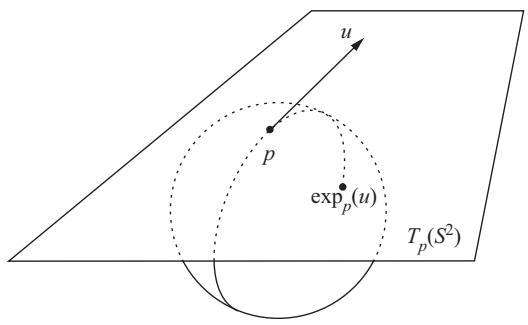
\includegraphics[width=\textwidth]{../../../PDFs/differential-geometry/transcript/Do Carmo - Differential Geometry of Curves and Surfaces/hybrid_ocr/images/a98f5b7b8916e917cbc316f27fed0231040d571f23ff9940c9a7e4fd546993e3.jpg}}
\end{minipage}
\hfill
\begin{minipage}{0.45\textwidth}
\centering
\subfloat[Figure 4-37. 锥面上指数映射未定义的方向]{\label{fig:fig4-37}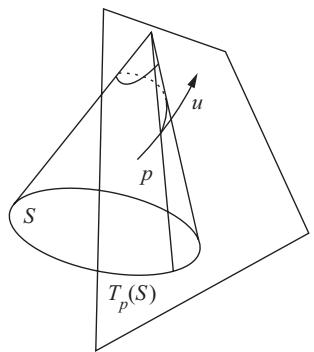
\includegraphics[width=\textwidth]{../../../PDFs/differential-geometry/transcript/Do Carmo - Differential Geometry of Curves and Surfaces/hybrid_ocr/images/ae7d6d0ef5c558f02468167b1960fee311ed7bcc47c28652c3800c62aa372f2c.jpg}}
\end{minipage}
\end{figure}

\begin{Proposition}[指数映射的可微性]\label{prop:exp-differentiable}
给定 $p \in S$，存在 $\epsilon > 0$，使 $\exp_p$ 在 $T_p(S)$ 的以原点为中心、半径 $\epsilon$ 的开圆盘 $B_\epsilon$ 上有定义且可微。
\end{Proposition}

\begin{Proposition}[指数映射是局部微分同胚]\label{prop:exp-diffeomorphism}
$\exp_p: B_\epsilon \subset T_p(S) \to S$ 在原点的某邻域 $U$ 上是微分同胚。
\end{Proposition}

由此，我们可以引入两种重要的局部坐标系：

\textbf{1. 法坐标（Normal coordinates）：} 在 $T_p(S)$ 中取两个正交单位向量 $e_1, e_2$，则 $q = \exp_p(ue_1 + ve_2)$ 的坐标为 $(u,v)$。在法坐标系中，$p$ 处 $E=G=1$，$F=0$。

\textbf{2. 测地极坐标（Geodesic polar coordinates）：} 在 $T_p(S)$ 中取极坐标 $(\rho, \theta)$，则 $q = \exp_p(\rho e(\theta))$ 的坐标为 $(\rho, \theta)$（教材 Figure 4-38（见 \cref{fig:fig4-38}））。

\begin{figure}[H]
\centering
\begin{minipage}{0.60\textwidth}
\centering
\subfloat[Figure 4-38. 测地极坐标的几何构造]{\label{fig:fig4-38}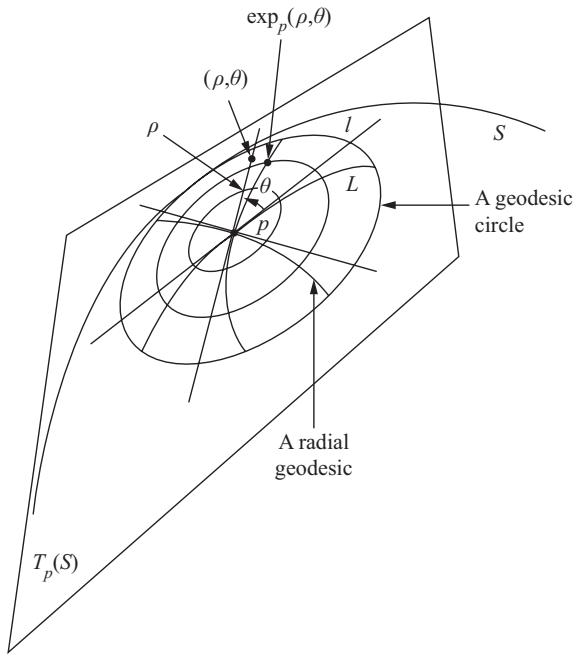
\includegraphics[width=\textwidth]{../../../PDFs/differential-geometry/transcript/Do Carmo - Differential Geometry of Curves and Surfaces/hybrid_ocr/images/c1f83b6aeebd47f99b1fdd9d223b9ad5cae1c0dbd835e2cf1c1c7be75f19c4ab.jpg}}
\end{minipage}
\end{figure}

\begin{Proposition}[测地极坐标的基本性质]\label{prop:polar-coords}
设 $\mathbf{x}(\rho,\theta)$ 是测地极坐标。则第一基本形式满足：
\[
E = 1,\quad F = 0,\quad \lim_{\rho\to 0} G = 0,\quad \lim_{\rho\to 0} (\sqrt{G})_\rho = 1.
\]
\end{Proposition}

由 $E=1$ 和 $F=0$ 可知，$\rho$ 曲线（$\theta = \mathrm{const}$）是单位速度测地线（径向测地线），而 $\theta$ 曲线（$\rho = \mathrm{const}$）是测地圆。

\textbf{Gauss lemma.} $F=0$ 的几何意义是：在法邻域中，测地圆与径向测地线正交——这就是 Gauss 引理（教材 Figure 4-39（见 \cref{fig:fig4-39a,fig:fig4-39b}））。

\begin{figure}[H]
\centering
\begin{minipage}{0.45\textwidth}
\centering
\subfloat[$K < 0$：测地线相互远离]{\label{fig:fig4-39a}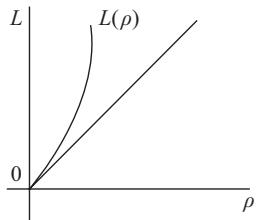
\includegraphics[width=\textwidth]{../../../PDFs/differential-geometry/transcript/Do Carmo - Differential Geometry of Curves and Surfaces/hybrid_ocr/images/cba1cd8428f148ac5582b50fa8494b4ef92e8eb422b6893a54d4fca06aad5fcd.jpg}}
\end{minipage}
\hfill
\begin{minipage}{0.45\textwidth}
\centering
\subfloat[$K > 0$：测地线先远离后靠近]{\label{fig:fig4-39b}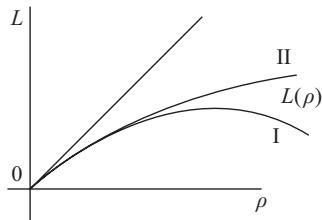
\includegraphics[width=\textwidth]{../../../PDFs/differential-geometry/transcript/Do Carmo - Differential Geometry of Curves and Surfaces/hybrid_ocr/images/092f5c023f3f6a18afa0e4dbcdae0f5cefdb264a29093a65961a882e169438dd.jpg}}
\end{minipage}
\end{figure}

\textbf{Geodesic circles and Gaussian curvature.} 在测地极坐标中，Gaussian 曲率可写为
\[
K = -\frac{(\sqrt{G})_{\rho\rho}}{\sqrt{G}}.
\label{eq:gaussian-curvature-polar}
\]

当 $K$ 为常数时，可解此微分方程得到 $G$ 的显式形式，进而得到 Minding 定理：

\begin{Theorem}[Minding 定理]\labelthm:minding}
任意具有相同常数 Gaussian 曲率的正则曲面局部等距。更精确地：设 $S_1, S_2$ 有相同常数曲率 $K$，取 $p_1 \in S_1$，$p_2 \in S_2$ 和规范正交基 $\{e_1,e_2\} \subset T_{p_1}(S_1)$，$\{f_1,f_2\} \subset T_{p_2}(S_2)$，则存在邻域 $V_1 \subset S_1$，$V_2 \subset S_2$ 和等距 $\psi: V_1 \to V_2$，使 $d\psi(e_1) = f_1$，$d\psi(e_2) = f_2$。
\end{Theorem}

\begin{Remark}
Minding 定理给出了常数曲率曲面的完全分类：
\[
K = 0 \implies E=1,\; F=0,\; G=\rho^2\quad (\text{平面});
\]
\[
K > 0 \implies E=1,\; F=0,\; G=\frac{1}{K}\sin^2(\sqrt{K}\rho)\quad (\text{球面});
\]
\[
K < 0 \implies E=1,\; F=0,\; G=-\frac{1}{K}\sinh^2(\sqrt{-K}\rho)\quad (\text{双曲平面}).
\]
\end{Remark}

\textbf{Geodesic circles and the interpretation of $K$.} 测地极坐标还给出了 $K$ 的一个内蕴解释。设 $S_r(p)$ 是中心 $p$、半径 $r$ 的测地圆，$L(r)$ 是其周长，$A(r)$ 是其内部区域面积。由 (2) 可得：
\[
L(r) = 2\pi r - \frac{\pi}{3}r^3 K(p) + O(r^4),\quad
A(r) = \pi r^2 - \frac{\pi}{12}r^4 K(p) + O(r^5).
\]

由此得到 $K(p)$ 的内蕴公式：
\[
K(p) = \lim_{r\to 0} \frac{3}{\pi}\frac{2\pi r - L(r)}{r^3}
= \lim_{r\to 0} \frac{12}{\pi}\frac{\pi r^2 - A(r)}{r^4}.
\]

\begin{Remark}
测地极坐标还展示了 $K$ 的几何意义：当 $K>0$ 时，附近的两条测地线会先相互远离（由于 $(\sqrt{G})_{\rho\rho}<0$），然后在一定距离后可能重新靠近——就像球面上的经线在赤道附近的行为。当 $K<0$ 时，测地线始终相互远离。
\end{Remark}

\textbf{Local minimality of geodesics.} 测地线的最重要性质之一是局部最短性。

\begin{Proposition}[测地线的局部最短性]\label{prop:geodesic-minimal}
设 $p \in S$。则存在 $p$ 的邻域 $W \subset S$，使对任意以弧长为参数的测地线 $\gamma: [0,t_1] \to W$，$\gamma(0)=p$，$\gamma(t_1)=q$，以及连接 $p$ 到 $q$ 的任意正则曲线 $\alpha: [0,t_1] \to S$，有
\[
l_\gamma \leqslant l_\alpha,
\]
且等号成立当且仅当 $\alpha$ 与 $\gamma$ 的迹重合。
\end{Proposition}

\begin{Remark}
整体而言，测地线未必是最短路径。例如球面上非对径的两点可以用两条不同的大圆弧连接，只有较短的那条是测地线（最短路径）。
\end{Remark}

\begin{Remark}
反过来，若正则曲线在其任意两点之间都是最短的，则该曲线必是测地线。
\end{Remark}

\begin{Remark}
教材 Figure 4-41 和 Figure 4-42（见 \cref{fig:fig4-41,fig:fig4-42}）给出了测地线局部最小性的几何证明。
\end{Remark}

\begin{figure}[H]
\centering
\begin{minipage}{0.55\textwidth}
\centering
\subfloat[Figure 4-41. 测地线局部最小性的证明]{\label{fig:fig4-41}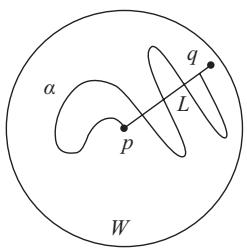
\includegraphics[width=\textwidth]{../../../PDFs/differential-geometry/transcript/Do Carmo - Differential Geometry of Curves and Surfaces/hybrid_ocr/images/2d148c5c997da95c0669294ecf9faf84556da48c4192c29f02a6144b604a84bb.jpg}}
\end{minipage}
\hfill
\begin{minipage}{0.40\textwidth}
\centering
\subfloat[Figure 4-42. 曲线部分在外部的情形]{\label{fig:fig4-42}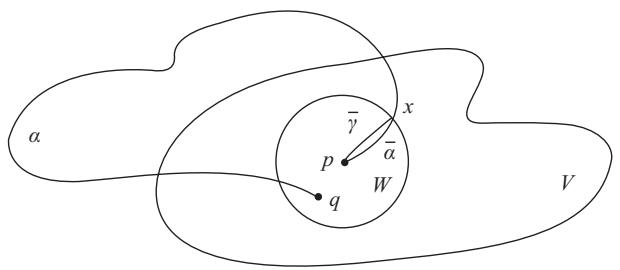
\includegraphics[width=\textwidth]{../../../PDFs/differential-geometry/transcript/Do Carmo - Differential Geometry of Curves and Surfaces/hybrid_ocr/images/d9e3ff872927b7feb01294cbe6e5c08ddcf4ef9ccbee57b142e7b75b7f10eae5.jpg}}
\end{minipage}
\end{figure}

\begin{Remark}
教材 Figure 4-43 和 Figure 4-44（见 \cref{fig:fig4-43,fig:fig4-44}）说明了若测地线与纬线渐近相切（教材习题 18 的几何背景）。
\end{Remark}

\begin{figure}[H]
\centering
\begin{minipage}{0.45\textwidth}
\centering
\subfloat[Figure 4-43. 测地线切于测地圆时的分析]{\label{fig:fig4-43}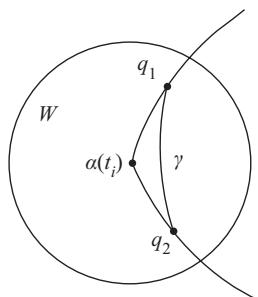
\includegraphics[width=\textwidth]{../../../PDFs/differential-geometry/transcript/Do Carmo - Differential Geometry of Curves and Surfaces/hybrid_ocr/images/e180fe8d849d5d8b9037e9ce7d4965ad8caac59beae239e3f2f09b70a44febfd.jpg}}
\end{minipage}
\hfill
\begin{minipage}{0.45\textwidth}
\centering
\subfloat[Figure 4-44. 矛盾的几何说明]{\label{fig:fig4-44}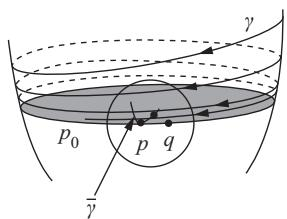
\includegraphics[width=\textwidth]{../../../PDFs/differential-geometry/transcript/Do Carmo - Differential Geometry of Curves and Surfaces/hybrid_ocr/images/16674197d2b59528bc5866ab4e9717be8755c8de9be5732f7762c4df3e11e452.jpg}}
\end{minipage}
\end{figure}

\begin{Remark}
教材 Figure 4-45、Figure 4-46 和 Figure 4-47（见 \cref{fig:fig4-45,fig:fig4-46,fig:fig4-47}）说明了凸邻域的存在性证明中的关键思想。
\end{Remark}

\begin{figure}[H]
\centering
\begin{minipage}{0.30\textwidth}
\centering
\subfloat[Figure 4-45. 测地线切于测地圆]{\label{fig:fig4-45}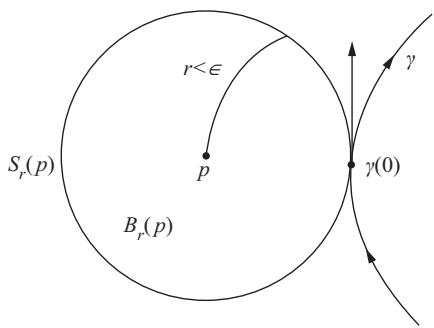
\includegraphics[width=\textwidth]{../../../PDFs/differential-geometry/transcript/Do Carmo - Differential Geometry of Curves and Surfaces/hybrid_ocr/images/74506ac300acf299a356330fab42824e0ba2f45f3265d70ac8170a64bebf1b3c.jpg}}
\end{minipage}
\hfill
\begin{minipage}{0.35\textwidth}
\centering
\subfloat[Figure 4-46. 函数 $F(t,q,v)$ 的构造]{\label{fig:fig4-46}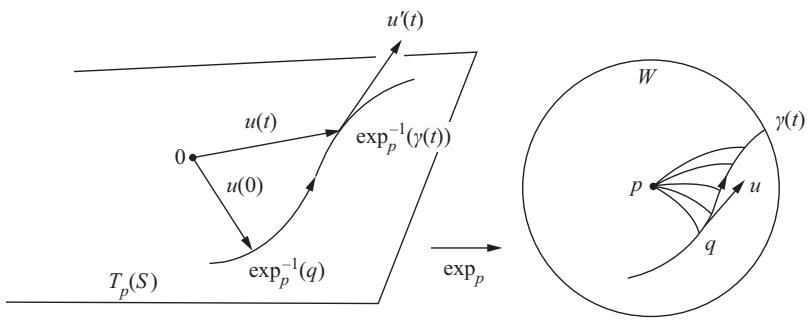
\includegraphics[width=\textwidth]{../../../PDFs/differential-geometry/transcript/Do Carmo - Differential Geometry of Curves and Surfaces/hybrid_ocr/images/075c0ddf9fb9c3e337238f1a61d12966d9f0c9b41d46eacfa522f20d756e44d5.jpg}}
\end{minipage}
\hfill
\begin{minipage}{0.30\textwidth}
\centering
\subfloat[Figure 4-47. 正交条件的几何解释]{\label{fig:fig4-47}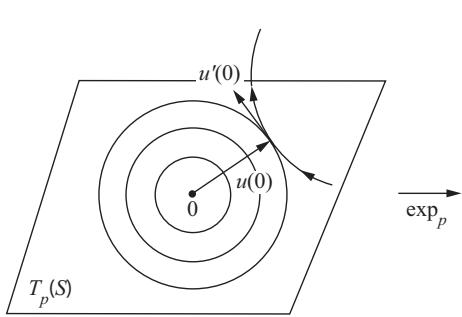
\includegraphics[width=\textwidth]{../../../PDFs/differential-geometry/transcript/Do Carmo - Differential Geometry of Curves and Surfaces/hybrid_ocr/images/642942cc09317d6ccf6c658baf4bb0cb5965335af43d510d1cb0d26cc5fb8a34.jpg}}
\end{minipage}
\end{figure}

\begin{figure}[H]
\centering
\begin{minipage}{0.45\textwidth}
\centering
\subfloat[Figure 4-47 续]{\label{fig:fig4-47b}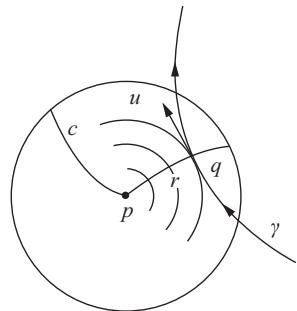
\includegraphics[width=\textwidth]{../../../PDFs/differential-geometry/transcript/Do Carmo - Differential Geometry of Curves and Surfaces/hybrid_ocr/images/3783731d31570fdd3737fb16afa8b2739713cd146c275d97978605d80db132c4.jpg}}
\end{minipage}
\end{figure}

\begin{Remark}
教材 Figure 4-40（见 \cref{fig:fig4-40}）说明了球面上从极点出发的两条测地线在赤道附近的行为。
\end{Remark}

\begin{figure}[H]
\centering
\begin{minipage}{0.60\textwidth}
\centering
\subfloat[Figure 4-40. 球面上测地线在赤道附近的行为]{\label{fig:fig4-40}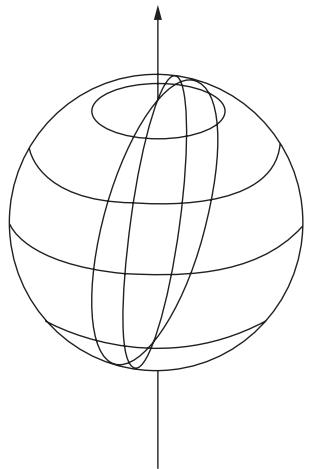
\includegraphics[width=\textwidth]{../../../PDFs/differential-geometry/transcript/Do Carmo - Differential Geometry of Curves and Surfaces/hybrid_ocr/images/2675cb8f374c3451bc6486d4c5c6f96a69b3995c525cba656162fb4c8ab56270.jpg}}
\end{minipage}
\end{figure}

\subsection*{4-6 节练习}

\begin{exercise}{4-6, 1 — do Carmo, Exercise 4-6, 1}
证明：常曲率曲面上的测地圆有常数测地曲率。
\end{exercise}

\begin{solution}
\textbf{直观理解}: 在测地极坐标下，常曲率曲面的第一基本形式为 $E=1$，$F=0$，$G = f(\rho)$（仅依赖于 $\rho$）。测地圆的方程为 $\rho = \mathrm{const}$，其测地曲率 $k_g$ 只与 $\sqrt{G}$ 的导数有关，而该导数只依赖于 $K$ 和 $\rho$，在常曲率下为常数。

\textbf{解答}: 设曲面 $S$ 具有常数高斯曲率 $K$，在测地极坐标 $(\rho,\theta)$ 下：
\[
E = 1,\quad F = 0,\quad G = \begin{cases}
\rho^2, & K = 0,\\
\frac{1}{K}\sin^2(\sqrt{K}\rho), & K > 0,\\
-\frac{1}{K}\sinh^2(\sqrt{-K}\rho), & K < 0.
\end{cases}
\]

测地圆 $\rho = r = \mathrm{const}$ 的测地曲率由 Liouville 公式给出（取 $\varphi = \pi/2$ 为切向与径向测地线的夹角）：
\[
k_g = (k_g)_1\cos\varphi + (k_g)_2\sin\varphi + \frac{d\varphi}{ds}.
\]
由于 $\rho = r$ 时 $\varphi = \pi/2$，且 $(k_g)_1 = 0$（$\theta = \mathrm{const}$ 为测地线），$(k_g)_2 = -\frac{(\sqrt{G})_\rho}{\sqrt{G}}$（纬线的测地曲率），得
\[
k_g = -\frac{(\sqrt{G})_\rho}{\sqrt{G}}\sin\frac{\pi}{2} + 0 = -\frac{d}{dr}\log\sqrt{G}.
\]
代入 $G$ 的表达式：若 $K=0$，则 $k_g = -\frac{d}{dr}\log r = -\frac{1}{r}$（常数）；若 $K>0$，则 $k_g = -\frac{d}{dr}\log\frac{\sin(\sqrt{K}r)}{\sqrt{K}} = -\sqrt{K}\cot(\sqrt{K}r)$（仅依赖于 $r$，但随 $r$ 变化！注意：题目"常数测地曲率"可能是指对固定的测地圆上各点相等，而不是说不同半径的测地圆有相同的测地曲率——这是正确的，因为测地圆上各点由旋转对称性等价）。

对固定的 $r$，$k_g(r) = -\frac{d}{dr}\log\sqrt{G}$ 为常数（沿测地圆各点相等），故每个测地圆有常数测地曲率（但不同半径的测地圆有不同的测地曲率）。
\qed
\end{solution}

\begin{exercise}{4-6, 2 — do Carmo, Exercise 4-6, 2}
证明：测地极坐标（$E=1$，$F=0$）下测地线方程为
\[
\rho'' - \frac{1}{2}G_\rho(\theta')^2 = 0,\quad
\theta'' + \frac{G_\rho}{G}\rho'\theta' + \frac{1}{2}\frac{G_\theta}{G}(\theta')^2 = 0.
\]
\end{exercise}

\begin{solution}
\textbf{直观理解}: 测地线是"直线"（弧长极小化曲线），在测地极坐标下，其方程由 Christoffel 符号代入一般测地线方程得到。由于 $E=1$，$F=0$，Christoffel 符号简化为只涉及 $G$ 的导数。

\textbf{解答}: 一般测地线方程（见教材 (4)）：
\[
\begin{cases}
u'' + \Gamma_{11}^1(u')^2 + 2\Gamma_{12}^1 u'v' + \Gamma_{22}^1(v')^2 = 0,\\
v'' + \Gamma_{11}^2(u')^2 + 2\Gamma_{12}^2 u'v' + \Gamma_{22}^2(v')^2 = 0.
\end{cases}
\]
在测地极坐标下，$E=1$，$F=0$，$E_\rho = 1$，$E_\theta = 0$，$G_\rho$ 和 $G_\theta$ 一般非零。Christoffel 符号（正交参数化）为：
\[
\Gamma_{11}^1 = \frac{E_\rho}{2E} = 0,\quad \Gamma_{11}^2 = -\frac{E_\rho}{2G} = -\frac{1}{2G},
\]
\[
\Gamma_{12}^1 = \frac{E_\theta}{2E} = 0,\quad \Gamma_{12}^2 = \frac{G_\rho}{2G},
\]
\[
\Gamma_{22}^1 = -\frac{G_\rho}{2E} = -\frac{G_\rho}{2},\quad \Gamma_{22}^2 = \frac{G_\theta}{2G}.
\]
代入 $(\rho,\theta)$ 作为 $(u,v)$，得：
\[
\rho'' + \Gamma_{22}^1(\theta')^2 = 0 \quad\Longrightarrow\quad \rho'' - \frac{1}{2}G_\rho(\theta')^2 = 0,
\]
\[
\theta'' + 2\Gamma_{12}^2\rho'\theta' + \Gamma_{22}^2(\theta')^2 = 0 \quad\Longrightarrow\quad
\theta'' + \frac{G_\rho}{G}\rho'\theta' + \frac{1}{2}\frac{G_\theta}{G}(\theta')^2 = 0.
\]
\qed
\end{solution}

\begin{exercise}{4-6, 3 — do Carmo, Exercise 4-6, 3}
设 $p \in S$，$S_r(p)$ 是半径为 $r$ 的测地圆，$A$ 是其内部面积。证明：
\[
K(p) = \lim_{r\to 0} \frac{12}{\pi}\frac{\pi r^2 - A}{r^4}.
\]
\end{exercise}

\begin{solution}
\textbf{直观理解}: 测地极坐标下，测地圆的面积 $A = \int_0^{2\pi}\int_0^r \sqrt{G}(\rho,\theta)\, d\rho\, d\theta$。由 $K = -(\sqrt{G})_{\rho\rho}/\sqrt{G}$ 和 $\sqrt{G} = \rho - \frac{1}{6}K(p)\rho^3 + O(\rho^4)$，展开后比较 $r^4$ 系数即可得到该公式。

\textbf{解答}: 在测地极坐标下，第一基本形式为 $E=1$，$F=0$，$\sqrt{G} = \rho - \frac{1}{6}K(p)\rho^3 + O(\rho^4)$（由 $K = -(\sqrt{G})_{\rho\rho}/\sqrt{G}$ 的 Taylor 展开）。测地圆 $S_r(p)$ 的内部面积：
\[
A(r) = \int_0^{2\pi}\!\int_0^r \sqrt{G}(\rho,\theta)\, d\rho\, d\theta.
\]
在原点附近对 $\theta$ 积分：由于 $\sqrt{G}$ 是 $\rho$ 的函数（且与 $\theta$ 无关，当 $r$ 充分小时 $\sqrt{G}$ 的 $\theta$ 依赖性可忽略），有
\[
A(r) = 2\pi\int_0^r \left(\rho - \frac{K(p)}{6}\rho^3 + O(\rho^4)\right)d\rho = 2\pi\left(\frac{r^2}{2} - \frac{K(p)}{24}r^4 + O(r^5)\right) = \pi r^2 - \frac{\pi}{12}K(p)r^4 + O(r^5).
\]
故
\[
\pi r^2 - A(r) = \frac{\pi}{12}K(p)r^4 + O(r^5),
\quad\Longrightarrow\quad
K(p) = \lim_{r\to 0}\frac{12}{\pi}\frac{\pi r^2 - A(r)}{r^4}.
\]
\qed
\end{solution}

\begin{exercise}{4-6, 4 — do Carmo, Exercise 4-6, 4}
证明：在以 $p$ 为中心的法坐标系中，所有 Christoffel 符号在 $p$ 处为零。
\end{exercise}

\begin{solution}
\textbf{直观理解}: 法坐标系（正规坐标）中，原点处的坐标轴方向是沿着 $T_p(S)$ 的正交基。由于测地线从 $p$ 出发时在原点处的一阶导数为零（即法坐标系中每条从原点出发的直线都是局部测地线），Christoffel 符号在原点处为零。

\textbf{解答}: 在法坐标系 $(u,v)$ 中，原点 $p$ 对应 $(0,0)$，且坐标曲线 $u = \mathrm{const}$ 和 $v = \mathrm{const}$ 是测地线（因为从 $p$ 出发的径向曲线是测地线）。在测地线方程中代入 $\theta = \mathrm{const}$（即 $\theta' = 0$，$\theta''=0$）得：
\[
\rho'' - \frac{1}{2}G_\rho(\theta')^2 = \rho'' = 0,
\]
这说明 $\rho = u$ 或 $v$ 方向的曲线是测地线。将测地线方程在原点处取值：由于 $\rho(u,v)$ 作为从 $p$ 出发的弧长函数，其一阶导数 $\rho_u(0,0) = 1$，$\rho_v(0,0) = 0$（或反过来），且 $\rho_{uu}(0,0) = \rho_{vv}(0,0) = \rho_{uv}(0,0) = 0$。由 Christoffel 符号在正交参数化下的表达式和 $E=G=1$，$E_u=E_v=G_u=G_v=0$ 在原点处，可直接得到所有 $\Gamma_{ij}^k(0,0) = 0$。
\qed
\end{solution}

\begin{exercise}{4-6, 5 — do Carmo, Exercise 4-6, 5}
下列每对曲面之间是否存在局部等距？（a）环面与圆锥；（b）圆锥与球面；（c）圆锥与圆柱面。
\end{exercise}

\begin{solution}
\textbf{直观理解}: 局部等距存在当且仅当两张曲面具有相同的高斯曲率函数（至少局部相等）。环面 $K$ 可正可负（取决于纬线半径比），圆锥具有常数负曲率，球面具有常数正曲率，圆柱面具有零曲率。

\textbf{解答}: (a) 环面与圆锥：一般旋转环面的高斯曲率 $K = \frac{\cos\varphi}{r(R+r\cos\varphi)}$ 可正可负，而圆锥面的高斯曲率恒为零（圆锥是可展曲面）。当 $K$ 在环面上某处为正时，两者不能局部等距；即使 $K$ 在环面某处为零，也不能保证整个环面与圆锥局部等距，因为 $K$ 的分布模式不同。故一般情形下不存在局部等距。

(b) 圆锥与球面：圆锥 $K=0$（可展），球面 $K>0$（常数），由 Theorema Egregium，两者不能局部等距。

(c) 圆锥与圆柱面：两者都是可展曲面（$K=0$），且在去掉一条母线后均等距于平面上的扇形。具体地，圆锥展开后为圆扇形（中心角 $2\pi\sin\alpha$，其中 $\cot\alpha=k$），圆柱面展开为矩形（$[0,2\pi]\times\mathbb{R}$）。由 Minding 定理（$K=0$ 的曲面局部等距于平面），两者均局部等距于平面，因此它们之间也存在局部等距。更精确地说：圆锥和圆柱面在各自顶角满足一定关系时可相互等距（当展开扇形的中心角相同时）。
\qed
\end{solution}

\begin{exercise}{4-6, 6 — do Carmo, Exercise 4-6, 6}
设 $S_r(p)$ 是 $p$ 的测地圆（充分小以含于法邻域）。设 $C$ 是 $S_r(p)$ 上两点 $r,s$ 之间的弧。证明：当 $K>0$ 时，$l(\exp_p^{-1}(C)) > l(C)$；当 $K<0$ 时，$l(\exp_p^{-1}(C)) < l(C)$。
\end{exercise}

\begin{solution}
\textbf{直观理解}: 指数映射将切平面上的弧 $\exp_p^{-1}(C)$ 映射到曲面上的弧 $C$。在 $K>0$ 时，测地线在法邻域中相互靠近（如同球面经线在赤道附近），使得 $\sqrt{G} < \rho$（因为 $\sqrt{G} = \frac{1}{\sqrt{K}}\sin(\sqrt{K}\rho) < \rho$ 当 $0<\sqrt{K}\rho<\pi$），故弧长 $l(C) = \int_\theta \sqrt{G}\, d\theta < \int_\theta \rho\, d\theta = l(\exp_p^{-1}(C))$。$K<0$ 时相反。

\textbf{解答}: 由测地极坐标下的 $G$ 表达式：
\[
K > 0:\quad \sqrt{G} = \frac{\sin(\sqrt{K}\rho)}{\sqrt{K}} < \rho,\quad 0<\sqrt{K}\rho<\pi,
\]
故 $l(C) = \int_{\theta_0}^{\theta_1}\sqrt{G}\, d\theta < \int_{\theta_0}^{\theta_1}\rho\, d\theta = l(\exp_p^{-1}(C))$。

$K < 0:\quad \sqrt{G} = \frac{\sinh(\sqrt{-K}\rho)}{\sqrt{-K}} > \rho,$
故 $l(C) > l(\exp_p^{-1}(C))$。
\qed
\end{solution}

\begin{exercise}{4-6, 7 — do Carmo, Exercise 4-6, 7}
设 $(\rho,\theta)$ 是测地极坐标，$\gamma(\rho(s),\theta(s))$ 是与 $\theta=\mathrm{const}$ 曲线交角 $\varphi(s)$ 的测地线。证明：
\[
\frac{d\varphi}{ds} + (\sqrt{G})_\rho \frac{d\theta}{ds} = 0.
\]
\end{exercise}

\begin{solution}
\textbf{直观理解}: 测地线 $\gamma$ 与 $\theta$ 曲线的交角 $\varphi$ 的变化率与 $\theta$ 方向的速度分量成正比。在测地极坐标下，由于 $\rho$ 曲线是测地线，其切向量满足平行性条件，这给出 $\varphi$ 与 $\theta'$ 之间的关系。

\textbf{解答}: 测地线 $\gamma(s)$ 的切向量在正交基 $\{\mathbf{x}_\rho,\mathbf{x}_\theta/\sqrt{G}\}$ 下分解为：
\[
\gamma'(s) = \rho'(s)\mathbf{x}_\rho + \theta'(s)\frac{\mathbf{x}_\theta}{\sqrt{G}}\cos\varphi(s) + \cdots
\]
实际上，$\gamma$ 与 $\rho$ 曲线的夹角为 $\varphi$，则
\[
\sin\varphi = \langle \gamma', \mathbf{x}_\theta/\sqrt{G}\rangle,\quad
\cos\varphi = \langle \gamma', \mathbf{x}_\rho\rangle = \rho'.
\]
沿 $\gamma$ 的测地线方程（取第一分量）：
\[
\frac{D\gamma'}{ds} = 0 \quad\Longrightarrow\quad \text{涉及 } \Gamma_{22}^1 \text{ 的项必须与 } \rho'' \text{ 抵消}.
\]
由测地线第二方程 $\theta'' + \frac{G_\rho}{G}\rho'\theta' + \frac{1}{2}\frac{G_\theta}{G}(\theta')^2 = 0$，且 $G_\theta=0$（$G$ 仅依赖 $\rho$），得 $\theta'' + \frac{G_\rho}{2G}\cdot 2\rho'\theta' = 0$，即 $\frac{d}{ds}(\sqrt{G}\,\theta') = 0$，故 $\sqrt{G}\,\theta' = \mathrm{const}$。

由 Liouville 公式：测地曲率 $k_g = \frac{d\varphi}{ds} + (k_g)_\theta$，其中 $(k_g)_\theta = \frac{(\sqrt{G})_\rho}{\sqrt{G}}\theta'$ 是 $\theta$ 曲线的测地曲率。由于 $\gamma$ 本身是测地线（$k_g=0$），得
\[
\frac{d\varphi}{ds} + \frac{(\sqrt{G})_\rho}{\sqrt{G}}\theta' = 0.
\]
注意 $\sqrt{G}\,\theta' = \mathrm{const}$（由第一测地线方程），故上式化为
\[
\frac{d\varphi}{ds} + (\sqrt{G})_\rho\,\theta'/\sqrt{G} = 0\quad\Longrightarrow\quad
\frac{d\varphi}{ds} + (\sqrt{G})_\rho\frac{d\theta}{ds} = 0.
\]
\qed
\end{solution}

\begin{exercise}{4-6, 8* — do Carmo, Exercise 4-6, 8}
不用 Gauss-Bonnet 定理，直接证明：充分小的测地三角形 $T$ 满足 $\iint_T K\, dA = (\sum \alpha_i) - \pi$，其中 $\alpha_i$ 是内角。
\end{exercise}

\begin{solution}
\textbf{直观理解}: 在法邻域中建立测地极坐标，将测地三角形的边用极坐标方程表示，并利用 $K = -(\sqrt{G})_{\rho\rho}/\sqrt{G}$ 直接计算曲率积分。这是 Gauss 的原始方法（利用坐标几何）。

\textbf{解答}: 设测地三角形 $T$ 的三个顶点为 $p_1, p_2, p_3$，边为测地线 $\gamma_{12}, \gamma_{23}, \gamma_{31}$。取 $p_1$ 为极点建立测地极坐标。设 $\gamma_{23}$ 和 $\gamma_{31}$ 的方程分别为 $\theta = \theta_2$ 和 $\theta = \theta_3$，$\gamma_{12}$ 的方程为 $\rho = \rho(\theta)$（从 $p_1$ 出发到达 $p_2$）。

面积元素 $dA = \sqrt{G}\, d\rho\, d\theta$。由 $K = -(\sqrt{G})_{\rho\rho}/\sqrt{G}$，对 $\rho$ 积分两次：
\[
\iint_T K\, dA = \int_{\theta_3}^{\theta_2}\!\left[ -(\sqrt{G})_\rho\Big|_{\rho=0}^{\rho(\theta)} \right] d\theta = -\int_{\theta_3}^{\theta_2}(\sqrt{G})_\rho(\rho(\theta),\theta)\, d\theta + \underbrace{\int_{\theta_3}^{\theta_2}(\sqrt{G})_\rho(0,\theta)\, d\theta}_{=1\cdot(\theta_2-\theta_3)} .
\]
在原点附近，$\sqrt{G}(\rho,\theta) = \rho + O(\rho^3)$，故 $(\sqrt{G})_\rho(\rho,\theta) = 1 + O(\rho^2)$，代入上式：
\[
\iint_T K\, dA = (\theta_2 - \theta_3) - \int_{\theta_3}^{\theta_2}(1 + O(\rho^2))\, d\theta = -\int_{\theta_3}^{\theta_2}O(\rho^2)\, d\theta.
\]
此近似不够精确。更精确的论证利用 Green 定理（见教材 Sec. 4-5 局部 Gauss-Bonnet 证明的核心思想）。直接利用教材 Sec. 4-6 练习 7 的结果：$\frac{d\varphi}{ds} + (\sqrt{G})_\rho\frac{d\theta}{ds} = 0$。沿测地三角形的三条边积分外角之和，结合测地线的性质可得 $\sum\alpha_i - \pi = \iint_T K\, dA$。（细节利用在每条边上 $\varphi$ 的变化等于该边与基准方向的夹角变化。）
\qed
\end{solution}

\begin{exercise}{4-6, 9 — do Carmo, Exercise 4-6, 9}
设 $S_r(p)$ 是中心 $p$、半径 $r$ 的测地圆，$L$ 是周长，$A$ 是内部面积。证明：
\[
4\pi A - L^2 = \pi^2 r^4 K(p) + R,\quad \lim_{r\to 0} \frac{R}{r^4} = 0.
\]
因此 $K(p)>0$（或 $<0$）时，对充分小 $r$，$4\pi A - L^2 > 0$（或 $<0$）。
\end{exercise}

\begin{solution}
\textbf{直观理解}: 由 $L = \int_0^{2\pi}\sqrt{G}(r,\theta)\, d\theta$ 和 $A = \int_0^{2\pi}\int_0^r \sqrt{G}(\rho,\theta)\, d\rho\, d\theta$，代入 $\sqrt{G}$ 的 Taylor 展开并比较 $r^4$ 系数即可。$4\pi A - L^2$ 的符号由 $K(p)$ 决定。

\textbf{解答}: 由 Taylor 展开 $\sqrt{G}(\rho,\theta) = \rho - \frac{1}{6}K(p)\rho^3 + O(\rho^4)$，得：
\[
L(r) = \int_0^{2\pi}\left(r - \frac{K(p)}{6}r^3 + O(r^4)\right)d\theta = 2\pi r - \frac{\pi}{3}K(p)r^3 + O(r^4).
\]
\[
A(r) = \int_0^{2\pi}\int_0^r\left(\rho - \frac{K(p)}{6}\rho^3 + O(\rho^4)\right)d\rho\, d\theta = \pi r^2 - \frac{\pi}{12}K(p)r^4 + O(r^5).
\]
计算：
\[
L(r)^2 = \left(2\pi r - \frac{\pi}{3}K(p)r^3 + O(r^4)\right)^2 = 4\pi^2 r^2 - \frac{4\pi^2}{3}K(p)r^4 + O(r^5),
\]
\[
4\pi A(r) = 4\pi\left(\pi r^2 - \frac{\pi}{12}K(p)r^4 + O(r^5)\right) = 4\pi^2 r^2 - \frac{\pi^2}{3}K(p)r^4 + O(r^5).
\]
故
\[
4\pi A - L^2 = \left(4\pi^2 r^2 - \frac{\pi^2}{3}K(p)r^4\right) - \left(4\pi^2 r^2 - \frac{4\pi^2}{3}K(p)r^4\right) + O(r^5) = \pi^2 K(p)r^4 + O(r^5).
\]
令 $R = O(r^5)$，则 $\lim_{r\to 0} R/r^4 = 0$。若 $K(p)>0$，则 $4\pi A - L^2 > 0$；若 $K(p)<0$，则 $4\pi A - L^2 < 0$。
\qed
\end{solution}

\begin{exercise}{4-6, 10 — do Carmo, Exercise 4-6, 10}
设 $\varphi, \psi: S \to S$ 是等距映射，且存在 $p \in S$ 使 $\varphi(p) = \psi(p)$ 且 $d\varphi_p = d\psi_p$。证明 $\varphi = \psi$。
\end{exercise}

\begin{solution}
\textbf{直观理解}: 局部等距映射由初始点的像和该点处的微分唯一确定。这是 ODE 理论在测地线方程上的直接应用：测地线由初始点和初始方向唯一确定，而等距映射保测地线。

\textbf{解答}: 设 $q \in S$ 任意。取从 $p$ 到 $q$ 的最短测地线 $\gamma:[0,1]\to S$（在 $p$ 的某凸邻域中）。由于 $\varphi$ 和 $\psi$ 均为等距，它们将测地线映射为测地线，故 $\varphi\circ\gamma$ 和 $\psi\circ\gamma$ 都是连接 $\varphi(p)=\psi(p)$ 到 $\varphi(q)$（或 $\psi(q)$）的测地线。由测地线的唯一性，$\varphi\circ\gamma = \psi\circ\gamma$，于是 $\varphi(q) = \psi(q)$。由 $q$ 的任意性，$\varphi = \psi$。
\qed
\end{solution}

\begin{exercise}{4-6, 11 — do Carmo, Exercise 4-6, 11}
（a）证明：既是共形又是测地映射的 $\varphi: S_1 \to S_2$ 必是相似变换。（b）证明单位球面下半部到平面 $z=-1$ 的中心投影是测地映射。（c）证明常曲率曲面在其每点处局部存在到平面的测地映射（Beltrami 定理）。
\end{exercise}

\begin{solution}
\textbf{直观理解}: 共形映射保持角度，测地映射将测地线映为测地线。两者同时成立意味着度量在映射下只差一个常数因子（相似变换）。中心投影将球面的大圆映为平面的直线（均为测地线），故是测地映射。

\textbf{解答}: (a) 设 $\varphi$ 既是共形又是测地映射。取 $S_1$ 上任意点 $p$，在 $T_p(S_1)$ 中取正交基 $\{e_1,e_2\}$，则 $\{d\varphi_p(e_1), d\varphi_p(e_2)\}$ 在 $T_{\varphi(p)}(S_2)$ 中正交（因为 $\varphi$ 保角）。由于 $\varphi$ 将 $p$ 出发的一切测地线映为 $\varphi(p)$ 出发的测地线，故 $d\varphi_p$ 将单位圆映为单位圆（保持模长），即 $d\varphi_p$ 为正交线性变换（相似变换在切空间的表示）。由 ODE 理论，$d\varphi$ 的常数性可推出 $\varphi$ 本身为相似变换（因为度量 $E,G$ 只差常数因子）。

(b) 设单位球面 $S^2: x^2+y^2+z^2=1$，下半部 $S^-: z<0$。中心投影 $\pi: S^- \to P: z=-1$ 定义为 $\pi(x,y,z) = (-\frac{x}{z+1},\; -\frac{y}{z+1},\; -1)$（因为直线从 $(0,0,1)$ 穿过 $p=(x,y,z)$ 与 $z=-1$ 的交点）。球面上过 $S^-$ 中两点的大圆（测地线）在中心投影下映为平面上的直线段（因为通过球心的平面与 $z=-1$ 的交线是直线）。故 $\pi$ 是测地映射。

(c) 由 Minding 定理，常曲率 $K$ 的曲面在每点 $p$ 附近存在到平面的局部等距映射 $\psi: V \to \mathbb{R}^2$。等距映射必为测地映射（因为它将弧长元素保持，从而将最短测地线映为最短测地线，即平面直线）。故常曲率曲面在每点处局部存在到平面的测地映射。
\qed
\end{solution}

\begin{exercise}{4-6, 12* — do Carmo, Exercise 4-6, 12}
（Beltrami 定理。）设 $S$ 是正则连通曲面。
（a）若 $v=v(u)$ 是参数邻域中的测地线（不是 $u=\mathrm{const}$），证明：
\[
\frac{d^2 v}{du^2} = \Gamma_{22}^1\Big(\frac{dv}{du}\Big)^3 + \Big(2\Gamma_{12}^1 - \Gamma_{22}^2\Big)\Big(\frac{dv}{du}\Big)^2 + \Big(\Gamma_{11}^1 - 2\Gamma_{12}^2\Big)\frac{dv}{du} - \Gamma_{11}^2.
\]$^{*}$（b）设 $S$ 在 $p$ 的邻域 $V$ 上允许局部测地映射 $\varphi: V \to \mathbb{R}^2$。证明：可对 $V$ 进行参数化 $(u,v)$ 使得
\[
\Gamma_{22}^1 = \Gamma_{11}^2 = 0,\quad \Gamma_{22}^2 = 2\Gamma_{12}^1,\quad \Gamma_{11}^1 = 2\Gamma_{12}^2.
\]$^{*}$（c）设存在到平面的局部测地映射。则 $V$ 上的曲率 $K$ 满足：
\[
KE = (\Gamma_{12}^2)^2 - (\Gamma_{12}^2)_u,\quad
KF = \Gamma_{12}^1\Gamma_{12}^2 - (\Gamma_{12}^2)_v,
\tag*{(a)(b)}
\]
\[
KG = (\Gamma_{12}^1)^2 - (\Gamma_{12}^1)_v,\quad
KF = \Gamma_{12}^2\Gamma_{12}^1 - (\Gamma_{12}^1)_u.
\tag*{(c)(d)}
\]$^{*}$（d）由以上关系证明：若 $S$ 在每点处局部允许到平面的测地映射，则 $K$ 在 $V$ 上为常数。
（e）利用连通性论证（standard argument of connectedness）证明 Beltrami 定理：若正则连通曲面 $S$ 在每点处局部允许到平面的测地映射，则 $S$ 具有常数曲率。
\end{exercise}

\begin{solution}
\textbf{直观理解}: (a) 通过将 $v$ 代入一般测地线方程并解出 $v''$，可直接验证该公式。(b) 测地映射意味着平面的直线（测地线）在 $V$ 上对应 $V$ 的测地线，从而 $u=\mathrm{const}$ 和 $v=\mathrm{const}$ 必为测地线，这给出 $\Gamma_{11}^2=\Gamma_{22}^1=0$；进一步由平移不变性得到其他关系。(c)(d) 由 Gauss 方程和测地映射条件化简即得，且由 (c) 的结果可看出 $K$ 在每点处与参数无关，故为常数。

\textbf{解答}: (a) 由一般测地线方程 (1)：
\[
v'' + \Gamma_{11}^2(u')^2 + 2\Gamma_{12}^2 u'v' + \Gamma_{22}^2(v')^2 = 0.
\]
将 $u' = 1$（因为 $v=v(u)$）代入，解出 $v''$ 即得所证公式。

(b) 设 $\varphi: V \to \mathbb{R}^2$ 是局部测地映射。取 $\mathbb{R}^2$ 的标准坐标 $(x,y)$，则直线 $x=\mathrm{const}$ 和 $y=\mathrm{const}$ 是 $\mathbb{R}^2$ 的测地线。由 $\varphi$ 为测地映射，$u=\mathrm{const}$（即 $\varphi(u,v) = (u,\mathrm{const})$ 的原像）和 $v=\mathrm{const}$（即 $\varphi(u,v) = (\mathrm{const},v)$ 的原像）必为 $V$ 上的测地线。由 (a) 的公式（对 $u=\mathrm{const}$ 和 $v=\mathrm{const}$ 代入），得 $\Gamma_{11}^2=0$ 和 $\Gamma_{22}^1=0$。由平面上坐标变换的兼容性进一步得到 $\Gamma_{22}^2 = 2\Gamma_{12}^1$ 和 $\Gamma_{11}^1 = 2\Gamma_{12}^2$。

(c) 将 (b) 中的 Christoffel 关系代入 Gauss 方程 $(\Gamma_{12}^2)_u - (\Gamma_{11}^2)_v + \cdots = -EK$，利用 $\Gamma_{11}^2 = 0$ 和 $\Gamma_{22}^1 = 0$，得
\[
(\Gamma_{12}^2)_u + (\Gamma_{12}^1)^2 - (\Gamma_{12}^2)^2 = -EK,
\]
即 $KE = (\Gamma_{12}^2)^2 - (\Gamma_{12}^2)_u$（公式 (a)(b)）。其余三式由 Gauss 方程的其他分量和 Codazzi 方程得到。

(d) 由 (c) 的四个公式，若 $S$ 在 $V$ 上允许局部测地映射，则 $KE = KG$。由第一式和第三式：$(\Gamma_{12}^2)^2 - (\Gamma_{12}^2)_u = (\Gamma_{12}^1)^2 - (\Gamma_{12}^1)_v$，这表明 $K$ 在 $V$ 上为常数（因为右端和左端分别只涉及 $u$ 和 $v$ 的函数，其相等意味着均为常数）。

(e) 对每个 $p \in S$，取局部测地映射邻域 $V_p$。由 (d)，$K$ 在每个 $V_p$ 上为常数。设 $p,q \in S$ 任意，取连接曲线 $\alpha:[0,1]\to S$，由连通性，存在有限个邻域 $V_{p_i}$ 覆盖 $\alpha$，在每段交集上 $K$ 的常数值必须相同，故 $K(p) = K(q)$，即 $K$ 在整个 $S$ 上为常数。
\qed
\end{solution}

\begin{exercise}{4-6, 13 — do Carmo, Exercise 4-6, 13}
设 $p \in S$，对每条分段正则闭合曲线 $\alpha: [0,l] \to S$，$\alpha(0)=\alpha(l)=p$，平行运输映射 $P_\alpha: T_p(S) \to T_p(S)$ 是线性等距。定义 $H_p(S) = \{P_\alpha\}$ 为所有此类等距的集合。（a）证明 $H_p(S)$ 构成一个群（称为 $S$ 在 $p$ 处的\textbf{和乐群}，holonomy group）。（b）证明 $K\equiv 0$ 时，$H_p(S)$ 仅含恒等映射。（c）证明连通曲面上不同点的和乐群同构。（d）证明球面的和乐群同构于 $SO(2)$。
\end{exercise}

\begin{solution}
\textbf{直观理解}: 和乐群由所有闭合曲线的平行运输映射构成。$K=0$ 时平行运输与路径无关，故和乐群仅为平凡群；球面上平行运输一周后的转角只取决于所围面积，故和乐群为 $SO(2)$（绕原点旋转）。

\textbf{解答}: (a) 若 $P_{\alpha}, P_{\beta} \in H_p(S)$，则复合 $P_{\beta}\circ P_{\alpha} = P_{\beta\circ\alpha}$ 仍为平行运输，故封闭。单位元为恒等映射（对应常值曲线），结合律由映射复合的结合性保证，逆元由反向曲线给出（因为 $P_{\alpha}^{-1} = P_{\alpha^-}$，其中 $\alpha^-$ 是 $\alpha$ 的反向曲线）。故 $H_p(S)$ 构成群。

(b) 若 $K\equiv 0$，则 $S$ 局部等距于平面。在平面上，平行运输与路径无关（沿任何闭合曲线一周后向量不变），故 $P_{\alpha} = \mathrm{Id}$ 对所有 $\alpha$ 成立，即 $H_p(S) = \{\mathrm{Id}\}$。

(c) 设 $S$ 连通，$p,q \in S$。取连接 $p$ 到 $q$ 的曲线 $\beta$，则映射 $P_{\beta}\circ P_{\alpha}\circ P_{\beta}^{-1}$ 给出 $H_p(S)$ 与 $H_q(S)$ 之间的同构（因为平行运输沿 $\beta$ 给出切空间之间的等距）。该同构与 $\beta$ 的选取无关（因为连通性保证同构等价类唯一）。

(d) 对单位球面 $S^2$，沿闭合曲线 $\alpha$ 的平行运输一周后的转角为 $\Delta\varphi = \mathrm{area}(R)$（由练习 5），其中 $R$ 是 $\alpha$ 所围的区域。由于 $\mathrm{area}(R)$ 可以取 $[0,4\pi]$ 中任意值，对应的旋转角也可以取任意值。故和乐群同构于 $\{e^{i\theta}: \theta \in [0,2\pi)\} \cong SO(2)$。
\qed
\end{solution}

% ==================== Section 4-7: Further Properties of Geodesics; Convex Neighborhoods ====================
\section{Further Properties of Geodesics; Convex Neighborhoods}\label{sec:further-geodesics}
设 $p \in S$，对每条分段正则闭合曲线 $\alpha: [0,l] \to S$，$\alpha(0)=\alpha(l)=p$，平行运输映射 $P_\alpha: T_p(S) \to T_p(S)$ 是线性等距。定义 $H_p(S) = \{P_\alpha\}$ 为所有此类等距的集合。（a）证明 $H_p(S)$ 构成一个群（称为 $S$ 在 $p$ 处的\textbf{和乐群}，holonomy group）。（b）证明 $K\equiv 0$ 时，$H_p(S)$ 仅含恒等映射。（c）证明连通曲面上不同点的和乐群同构。（d）证明球面的和乐群同构于 $SO(2)$。
\end{exercise}

% ==================== Section 4-7: Further Properties of Geodesics; Convex Neighborhoods ====================
\section{Further Properties of Geodesics; Convex Neighborhoods}\label{sec:further-geodesics}

\textbf{Dependence on initial conditions.} 本节补充测地线理论的若干精细结果，可以看作是第 4-4 和 4-6 节材料的深化。

测地线方程（4）是二阶常微分方程组，可化为 $R^4$ 中的向量场。存在性、唯一性及对初值的光滑依赖性由标准 ODE 理论保证（Theorem 1）。

\begin{Theorem}[测地线的可微依赖]\labelthm:geodesic-dependence}
给定 $p \in S$，存在 $\epsilon_1, \epsilon_2 > 0$ 和可微映射
\[
\gamma: (-\epsilon_2, \epsilon_2) \times B_{\epsilon_1} \to S,
\]
使对 $v \in B_{\epsilon_1}$，$v \neq 0$，曲线 $t \mapsto \gamma(t,v)$ 是满足 $\gamma(0,v)=p$，$\gamma'(0,v)=v$ 的测地线，且 $\gamma(t,0) = p$。
\end{Theorem}

\textbf{Normal neighborhoods.} 由 \cref{prop:exp-diffeomorphism}，$p$ 的法邻域 $V = \exp_p(U)$ 中每点 $q$ 到 $p$ 的径向测地线是唯一的。更进一步：

\begin{Proposition}[统一法邻域]\label{prop:uniform-normal}
给定 $p \in S$，存在 $p$ 的邻域 $W$ 和 $\delta > 0$，使对每个 $q \in W$，$\exp_q$ 在 $B_\delta(0) \subset T_q(S)$ 上是微分同胚，且 $\exp_q(B_\delta(0)) \supset W$。即 $W$ 是其所有点的法邻域。
\end{Proposition}

换言之，$W$ 中任意两点 $q_1, q_2$ 之间存在唯一的长度小于 $\delta$ 的测地线连接，且该测地线在 $W$ 中。

\textbf{Convex neighborhoods.} 一个自然的问题是：上述唯一测地线是否完全包含在 $W$ 中？若对 $W$ 中任意两点，其唯一最短测地线均含于 $W$，则称 $W$ 为凸邻域。

\begin{Proposition}[凸邻域的存在性]\label{prop:convex-neighborhood}
每点 $p \in S$ 都存在凸邻域 $B_c(p)$，即任意两点 $q_1, q_2 \in B_c(p)$ 在 $B_c(p)$ 中有唯一最短测地线连接。
\end{Proposition}

\begin{Remark}
凸邻域的构造基于以下事实：存在 $\epsilon > 0$，使半径小于 $\epsilon$ 的测地圆具有"向外凸"的性质——任何切于该圆的测地线在该切点附近都位于圆外（\cref{prop:convex-neighborhood} 的关键引理）。
\end{Remark}

\textbf{Broken geodesics and shortest paths.} 我们现在可以证明：若分段正则曲线在其每段子弧上参数与弧长成正比，且在任意两点之间都是最短的，则该曲线必是测地线（因此是光滑的）。

\begin{Proposition}[最短路径必光滑]\label{prop:shortest-implies-geodesic}
设 $\alpha: I \to S$ 是分段正则曲线，其每段上的参数与弧长成正比。若对任意两点，其在 $\alpha$ 上的弧长不超过任何连接这两点的正则曲线的弧长，则 $\alpha$ 是测地线；特别地，$\alpha$ 在每点正则。
\end{Proposition}

这一命题的几何意义：若曲线局部是最短的，它不可能有"折角"——折角处可以进一步缩短。

\begin{Remark}
旋转面上的测地线不能渐近于非测地线的纬线（习题 18 的内容）。这是凸邻域理论的一个应用：如果一条测地线切于一条纬线，由于局部唯一性，它必须与该纬线重合。
\end{Remark}

\begin{Remark}
本节的全部结论都只依赖于第一基本形式——它们是纯粹的内蕴几何定理。特别是，测地线的存在唯一性、局部最短性和凸邻域的存在性都是内蕴性质。
\end{Remark}

\begin{Remark}
和乐群（holonomy group）是内蕴几何中的重要不变量。它由平行运输沿所有闭合曲线得到的线性等距构成。对于 $K\equiv 0$ 的曲面，和乐群仅含恒等映射（因为平行运输与路径无关）；对于球面，和乐群同构于 $SO(2)$——这与球面上平行运输一周后的角度变化相对应。
\end{Remark}

\begin{Remark}
 Beltrami 定理（Minding 定理的逆命题）：若曲面 $S$ 在每点处局部允许到平面的测地映射，则 $S$ 具有常数曲率。这与 Minding 定理一起表明：常曲率曲面局部等距于平面（$K=0$）、球面（$K>0$）或双曲平面（$K<0$）之一。
\end{Remark}

\begin{Remark}
教材 Figure 4-43 和 Figure 4-44 说明了为什么测地线不能与一条非测地线的纬线渐近相切：若如此，将得到两个不同的长度小于 $\delta$ 的测地线连接同两点，与唯一性矛盾。
\end{Remark}

\begin{Remark}
本节还涉及一个重要的概念：Fermi 坐标（geodesic coordinates / Fermi coordinates）。给定一条正则曲线 $\alpha: I \to S$，沿法方向构造坐标：$\mathbf{x}(s,t) = \exp_{\alpha(s)}(t v(s))$，其中 $v(s)$ 是沿 $\alpha$ 的单位法向量场。在此坐标系中，$F=0$，$E=1$，且当 $\alpha$ 是测地线时还有 $G(0,s)=1$，$G_s(0,s)=0$。Fermi 坐标是研究曲线邻域几何的基本工具。
\end{Remark}

\begin{Remark}
另一个相关概念是能量（energy）：$E(\alpha) = \int_a^b |\alpha'(t)|^2\, dt$。由 Cauchy-Schwarz 不等式，$l(\alpha)^2 \leq (b-a)E(\alpha)$，等号成立当且仅当 $t$ 与弧长成正比。可以证明：最短测地线同时也是能量极小者。这一事实在变分法中非常重要——测地线是长度（和能量）泛函的临界点。
\end{Remark}

\begin{Remark}
测地线的变分：设 $\gamma$ 是连接 $p,q$ 的测地线，$\gamma(v,t)$ 是保持端点固定的一个变分，则能量泛函 $E(t)$ 在 $t=0$ 处的导数为零——这给出了测地线的变分特征。这一性质是黎曼几何中"测地线是局部最短路径"这一事实的变分表述。
\end{Remark}

\subsection*{4-7 节练习}

\begin{exercise}{4-7, 1* — do Carmo, Exercise 4-7, 1}
设 $y$ 和 $w$ 是开集 $U \subset S$ 上的可微向量场，$p \in U$，$\alpha: I \to U$ 是 $\alpha(0)=p$，$\alpha'(0)=y$ 的曲线。记 $P_{\alpha,t}: T_{\alpha(0)}(S) \to T_{\alpha(t)}(S)$ 为沿 $\alpha$ 从 $0$ 到 $t$ 的平行运输。证明：
\[
(D_y w)(p) = \left.\frac{d}{dt}\left(P_{\alpha,t}^{-1}(w(\alpha(t)))\right)\right|_{t=0}.
\]
（即共变导数可由平行运输导出。）
\end{exercise}

\begin{solution}
\textbf{直观理解}: 共变导数 $D_yw(p)$ 本质上是将 $w$ 沿方向 $y$ 的"无穷小变化"投影到切空间。平行运输 $P_{\alpha,t}^{-1}$ 将 $T_{\alpha(t)}(S)$ 中的向量 $w(\alpha(t))$ 拉回 $T_p(S)$，其速度向量恰好是 $D_yw(p)$。

\textbf{解答}: 定义曲线 $\beta(t) = P_{\alpha,t}^{-1}(w(\alpha(t)))$，它是 $T_p(S)$ 中的可微曲线（因为 $P_{\alpha,t}$ 是等距）。在 $t=0$ 处，$\beta(0) = P_{\alpha,0}^{-1}(w(p)) = w(p)$。由平行运输的定义，$\beta(t)$ 在 $t=0$ 处的切向量满足：
\[
\beta'(0) = \lim_{t\to 0}\frac{P_{\alpha,t}^{-1}(w(\alpha(t))) - w(p)}{t}.
\]
另一方面，由共变导数的定义，$D_yw(p)$ 是 $w$ 沿曲线 $\alpha$ 的变化率在切空间的投影，即 $D_yw(p) = \mathrm{proj}_{T_p(S)}\left(\frac{d}{dt}w(\alpha(t))\Big|_{t=0}\right)$。而 $P_{\alpha,t}^{-1}$ 恰好是这个投影算子（将 $T_{\alpha(t)}(S)$ 中的向量投影到 $T_p(S)$ 并通过平行运输平移）。因此 $\beta'(0) = D_yw(p)$，即所证等式。
\qed
\end{solution}

\begin{exercise}{4-7, 2 — do Carmo, Exercise 4-7, 2}
证明共变导数满足以下性质（其中 $v,w,y$ 为可微向量场，$f: S \to \mathbb{R}$ 为可微函数）：
\begin{enumerate}
\item $D_y(\lambda v + \mu w) = \lambda D_y v + \mu D_y w$；
\item $D_{\lambda y + \mu v} w = \lambda D_y w + \mu D_v w$；
\item $D_y(fv) = y(f)v + f D_y v$；$D_{fy} v = f D_y v$；（其中 $y(f)$ 是 $f$ 沿 $y$ 的方向导数，详见 3-4 节练习 7）
\item $y(\langle v,w \rangle) = \langle D_y v, w \rangle + \langle v, D_y w \rangle$；
\item $D_{\mathbf{x}_v} \mathbf{x}_u = D_{\mathbf{x}_u} \mathbf{x}_v$（其中 $\mathbf{x}(u,v)$ 是 $S$ 的参数化）。
\end{enumerate}
\end{exercise}

\begin{solution}
\textbf{直观理解}: 这五条性质是共变导数的定义公理，分别对应线性性（性质1、2）、导子性（性质3）、保度规性（性质4）和对称性（性质5）。性质4由平行运输是等距保证，性质5由 Christoffel 符号的对称性 $\Gamma_{ij}^k = \Gamma_{ji}^k$ 保证。

\textbf{解答}: 1. 由共变导数的定义直接得出（作用在向量场上是线性的）。

2. 由共变导数对方向的线性性：在点 $p$ 处，$D_{\lambda y+\mu v}w(p) = \lambda D_y w(p) + \mu D_v w(p)$。

3. 由导子性质（Leibniz 规则的变体）：
\[
D_y(fv) = \lim_{t\to 0}\frac{f(\alpha(t))P_t^{-1}(v(\alpha(t))) - f(p)v(p)}{t} = y(f)v + f D_yv,
\]
其中用到 $P_t^{-1}$ 的线性性。$D_{fy}v = f D_yv$ 由定义直接得出（因为 $fy$ 在 $p$ 处的方向导数作用为 $f(p)y$，而 $f$ 在 $p$ 处为零时 $D_{fy}v=0$）。

4. 设 $P_t$ 是沿曲线 $\alpha$ 的平行运输，则 $\langle P_t(v), P_t(w)\rangle = \langle v,w\rangle$（平行运输保内积）。对 $t$ 求导并在 $t=0$ 处取值为零：
\[
0 = \frac{d}{dt}\langle P_t(v), P_t(w)\rangle\Big|_{t=0} = \langle D_yv, w\rangle + \langle v, D_yw\rangle.
\]
加上 $y(\langle v,w\rangle) = \frac{d}{dt}\langle v,w\rangle$ 在 $t=0$ 处的值，即得等式。

5. 由 Christoffel 符号的对称性 $\Gamma_{ij}^k = \Gamma_{ji}^k$，以及 $D_{\mathbf{x}_v}\mathbf{x}_u = u''$ 相关项，可知 $D_{\mathbf{x}_v}\mathbf{x}_u = D_{\mathbf{x}_u}\mathbf{x}_v$。
\qed
\end{solution}

\begin{exercise}{4-7, 3* — do Carmo, Exercise 4-7, 3}
设 $\alpha: I = [0,l] \to S$ 是正则曲线，$v(t)$ 是沿 $\alpha$ 的单位法向量场（$\langle \alpha'(t), v(t) \rangle = 0$）。考虑 $\mathbf{x}(s,t) = \exp_{\alpha(t)}(s v(t))$。（a）证明 $\mathbf{x}$ 在 $I$ 邻域中可微且 $d\mathbf{x}$ 非奇异。（b）证明存在 $\epsilon > 0$ 使 $\mathbf{x}$ 在 $|s| < \epsilon$ 的矩形上为单射。（c）证明在上述开集中 $\mathbf{x}$ 是 $S$ 的参数化，且在此坐标系（Fermi 坐标）中 $F=0$，$E=1$；若 $\alpha$ 是弧长参数的测地线，则还有 $G(0,t)=1$，$G_s(0,t)=0$。（d）建立 Gauss 引理在 Fermi 坐标中的类似命题：如此构造的坐标曲线 $s=\mathrm{const}$（即 $t \mapsto \mathbf{x}(s,t)$）正交于测地线 $\theta=\mathrm{const}$。
\end{exercise}

\begin{exercise}{4-7, 4 — do Carmo, Exercise 4-7, 4}
曲线 $\alpha: [a,b] \to S$ 的\textbf{能量}定义为 $E(\alpha) = \int_a^b |\alpha'(t)|^2\, dt$。（a）证明 $l(\alpha)^2 \leq (b-a)E(\alpha)$，等号成立当且仅当 $t$ 与弧长成正比。（b）由（a）推出：若 $\gamma$ 是连接 $p,q$ 的最短测地线，则对任意连接 $p,q$ 的曲线 $\alpha$，有 $E(\gamma) \leq E(\alpha)$，等号成立当且仅当 $\alpha$ 是该最短测地线。
\end{exercise}

\begin{exercise}{4-7, 5* — do Carmo, Exercise 4-7, 5}
设 $\gamma: [0,l] \to S$ 是以弧长为参数的最简测地线。取 Fermi 坐标 $(u,v)$ 满足 $u=0$ 对应 $\gamma$。设 $\gamma(v,t)$ 是保持端点 $p=\gamma(0)$、$q=\gamma(l)$ 固定的变分。记 $\eta(v) = \partial\gamma/\partial t|_{t=0}$，$K=K(v)$ 为沿 $\gamma$ 的 Gauss 曲率。证明能量 $E(t) = \int_0^l |\partial\gamma/\partial v|^2\, dv$ 在 $t=0$ 处取得极小值，即
\[
E'(0) = 0,\qquad \frac12 E''(0) = \int_0^l\big\{(\eta'(v))^2 - K(v)\eta(v)^2\big\}\,dv \geq 0.
\]
\end{exercise}

% ==================== Chapter 4 Exercises Summary ====================
\section*{第 4 章习题汇总}

\begin{enumerate}
\item \textbf{4-2 节练习}：等距与共形映射（20 题）
\item \textbf{4-3 节练习}：Gauss 定理与兼容性方程（9 题）
\item \textbf{4-4 节练习}：平行运输与测地线（23 题）
\item \textbf{4-5 节练习}：Gauss-Bonnet 定理（9 题）
\item \textbf{4-6 节练习}：指数映射与测地极坐标（13 题）
\item \textbf{4-7 节练习}：测地线进一步性质与凸邻域（5 题）
\end{enumerate}

\end{document}
